% !TeX root = robust_global_redistr.tex
\documentclass[aspectratio=169,xcolor=dvipsnames, 11pt,mathserif]{beamer} 
% !TeX root = robust_global_redistr.tex
% \documentclass[aspectratio=169,xcolor=dvipsnames, 11pt,mathserif]{beamer} 
% Put this line above % !TeX root = robust_global_redistr.tex
% \documentclass[aspectratio=169,xcolor=dvipsnames, 11pt,mathserif]{beamer} 
% Put this line above % !TeX root = robust_global_redistr.tex
% \documentclass[aspectratio=169,xcolor=dvipsnames, 11pt,mathserif]{beamer} 
% Put this line above \input{preamble_slides.tex} otherwise it may cause bug

%\documentclass[xcolor=dvipsnames,mathserif]{beamer} % this option has curvier math
%\documentclass[xcolor=dvipsnames,11pt]{beamer}
% Note: the color structure needs to be added here in the title. Now it recognizes all beamer % colors.

%%%%%%%%  PRESENTATION LAYOUT:
\usepackage{appendixnumberbeamer} % this package does not count the appendix pages. /!\ Inconstant behavior, sometimes bug.
\mode<presentation>
{
  \usetheme{Boadilla}
  \usecolortheme{lily} % lily is nice or orchid but not for definition
  \setbeamercovered{invisible}
  \setbeamertemplate{footline}{\raggedleft\insertframenumber~/~\inserttotalframenumber\hspace*{3pt}\vskip3pt} %this command shows frame number, not page number at bottom (means if using overlays, % frame number does not change)
%\setbeamertemplate{footline}[page number]  % this puts only page number on bottom
 \setbeamertemplate{navigation symbols}{t}  % this erases navigation symbols.
 \setbeamersize{text margin left=0.1cm, text margin right=0.1cm} % left=0.2cm
 \setbeamertemplate{frametitle}[default][center]
 \setbeamercolor{frametitle}{fg=black}
 \setbeamerfont{frametitle}{size=\large, series=\bfseries} % Modifies frame title font.
 \setbeamercolor{button}{fg=blue, bg=white}
 \setbeamertemplate{itemize item}[circle]
 \setbeamercolor{itemize item}{fg=black}
 \setbeamercolor{itemize/enumerate body}{fg=black}
 \setbeamerfont{framesubtitle}{series=\mdseries}
}

\renewcommand{\familydefault}{\rmdefault} %Options here are \ttdefault \ssdefault or \rmdefault.

% This defines actual color palette; 
\definecolor{blue}{RGB}{0,114,178}
\definecolor{orangered}{RGB}{213,94,0}
\definecolor{yellow}{RGB}{240,228,66}
\definecolor{green}{RGB}{0,158,115}
\definecolor{orange}{RGB}{230,159,0}

\hypersetup{
  colorlinks = false,
  linkbordercolor = {white},
  linkcolor = {blue}
}

%%% Color customization: where these colors are used. 
\colorlet{cwords}{blue} %this defines a color, stored under the name cwords that will be used and recognized in document.
\colorlet{cwordsc}{red} %color for contrast with some other word.
\colorlet{cwords2}{green} %2nd color for contrast with some other word.
\colorlet{cmath}{blue} %color for math in text.
%\everymath{\color{blue}} % This in conjunction with the everysel package sets color of math
\everydisplay{\color{blue}}


%%%%%%%%  PACKAGES USED:
\usepackage{amsmath}
\usepackage{setspace} % Only needed for spacing
\usepackage{changepage} % Only needed for local margin setting
\usepackage{mathpazo}% font, is overwritten by times
%\usepackage[hypertexnames=false]{hyperref} %This makes hyperref ``dumber'', and, hence, more robust! (otherwise sometimes the appendix links don't work).
\usepackage{hyperref}
\usepackage{multimedia}
\usepackage[english]{babel}
\usepackage{graphicx}
\usepackage[justification=centering]{caption}
%\usepackage{subfig}
\usepackage{subfloat}
\usepackage[en-US]{datetime2}
\usepackage{tabulary}
\usepackage{tabularx}
\usepackage{makecell} % multiline cells in tables
\usepackage{array,booktabs} % Needed for esttab tables according to the "inequality survey."
\newcommand{\sym}[1]{{#1}} % for symbols in Table
\usepackage[T1]{fontenc}
\usepackage[utf8]{inputenc}
\usepackage{times} % This is a different font.
\usepackage[overlay,absolute]{textpos}
%%%\usepackage{animate} % Animate graphs BUG
\setlength{\TPHorizModule}{1cm}
\setlength{\TPVertModule}{1cm}
\captionsetup[figure]{labelformat=empty} % removes caption prefix figure
\setlength{\itemsep}{\fill} % this is supposed to stretch items across full frame.
%\setlength{\parskip}{0.8\baselineskip} % This affects spacing between normal lines (not itemized).
\usepackage{colortbl} % For cell colors
\usepackage[final]{pdfpages}
\usepackage{caption}
\usepackage{subcaption}
%\captionsetup{justification   = raggedright,
%              singlelinecheck = false}
%\usepackage{adjustbox} % to use resizebox for tables size.
\usepackage[export]{adjustbox} % to use resizebox for tables size.
\usepackage{eurosym}
\usepackage{gensymb}
\usepackage{dsfont}
%\usepackage{enumitem}
%\setlist[itemize]{leftmargin=*} % remove margin from itemize

%% TIKZ
\usepackage{tikz}
% \usetikzlibrary{er, positioning,decorations.pathmorphing,calc}
% \usepackage{tikzscale}
% %% TIKZIT
% \usetikzlibrary{backgrounds}
% \usetikzlibrary{arrows}
% \usetikzlibrary{shapes,shapes.geometric,shapes.misc}
% % this style is applied by default to any tikzpicture included via \tikzfig
% \tikzstyle{tikzfig}=[baseline=-0.25em,scale=0.5]
% % these are dummy properties used by TikZiT, but ignored by LaTex
% \pgfkeys{/tikz/tikzit fill/.initial=0}
% \pgfkeys{/tikz/tikzit draw/.initial=0}
% \pgfkeys{/tikz/tikzit shape/.initial=0}
% \pgfkeys{/tikz/tikzit category/.initial=0}
% % standard layers used in .tikz files
% \pgfdeclarelayer{edgelayer}
% \pgfdeclarelayer{nodelayer}
% \pgfsetlayers{background,edgelayer,nodelayer,main}
% % style for blank nodes
% \tikzstyle{none}=[inner sep=0mm]
% % include a .tikz file
% \newcommand{\tikzfig}[1]{%
% {\tikzstyle{every picture}=[tikzfig]
% \IfFileExists{#1.tikz}
%   {\input{#1.tikz}}
%   {%
%     \IfFileExists{../figures/#1.tikz}
%       {\input{../figures/#1.tikz}}
%       {\tikz[baseline=-0.5em]{\node[draw=red,font=\color{red},fill=red!10!white] {\textit{#1}};}}%
%   }}%
% }
% % the same as \tikzfig, but in a {center} environment
% \newcommand{\ctikzfig}[1]{%
% \begin{center}\rm
%   \tikzfig{#1}
% \end{center}}
% % fix strange self-loops, which are PGF/TikZ default
% \tikzstyle{every loop}=[]
% \newcommand*\halfcirc{%
% %  \begin{tikzpicture}
% %  \draw[fill] (2,1)-- (90:1ex) arc (90:270:1ex) -- cycle ;
% %  \draw (2,1) circle (1ex);
% %  \end{tikzpicture}
% }
  
% \input{../latex/default.tikzstyles}


% \tikzset{every entity/.style={draw=black, fill=white}}
% \tikzset{comment/.style={draw=white, fill=white}}
% \tikzset{
% 	invisible/.style={opacity=0},
% 	visible on/.style={alt=#1{}{invisible}},
% 	alt/.code args={<#1>#2#3}{%
% 		\alt<#1>{\pgfkeysalso{#2}}{\pgfkeysalso{#3}} % \pgfkeysalso doesn't change the path
% 	},
% }

% Commands from template
\newcommand{\alrt}[1]{{\color{alert} #1}}
\newcommand{\alrtl}[1]{{\color{alert}\large #1}}
\newcommand{\alrtL}[1]{{\color{alert}\Large #1}}
\newcommand{\struc}[1]{{\color{structure} #1}}
\newcommand{\strucL}[1]{{\color{structure}\Large #1}}
\newcommand{\strucl}[1]{{\color{structure}\large #1}}
\newcommand{\dred}[1]{{\color{darkred} #1}}
\newcommand{\dredl}[1]{{\color{darkred}\large #1}}
\newcommand{\dredL}[1]{{\color{darkred}\Large #1}}
\newcommand{\altc}[1]{{\color{darkgreen}\textbf{#1}}}
\newcommand{\altcl}[1]{{\color{darkgreen}\textbf{\large #1}}}
\newcommand{\altcL}[1]{{\color{darkgreen}\textbf{\Large #1}}}
\newcommand{\hush}{\hushit}
\newcommand{\hushalrt}[1]{\hushit{{\color{alert} #1}}}
\newcommand{\hushalrtl}[1]{\hushit{{\large\color{alert} #1}}}
\newcommand{\hushalrtL}[1]{\hushit{{\Large\color{alert} #1}}}
\newcommand{\hushstruc}[1]{\hushit{{\color{structure} #1}}}
\newcommand{\hushstrucl}[1]{\hushit{{\large\color{structure} #1}}}
\newcommand{\hushstrucL}[1]{\hushit{{\Large\color{structure} #1}}}


\setbeamertemplate{caption}[numbered]

%%%%%%% SIGN NOBEL PRIZE %%%%%%%%
\usepackage{wasysym}
\newcommand{\nobel}{$\taurus$} % other possibilities:\logof\odot\varocircle\taurus\kreuz
\newcommand{\Nobel}[1]{$\taurus_{#1}$}
\newcommand{\Leontief}[1]{$\logof_{#1}$}
\newcommand{\leontief}{$\logof_$}

%%%%%%%%%SECTION TITLES DISPLAYED ON FULL PAGE %%%%%%%%%%
%%%%%%%%%%%%%%%%%%%%%%%%%%%%%%%%%%%%%%%%%%%
\AtBeginSection[]{
  \begin{frame}
  \vfill
  \centering
  \begin{beamercolorbox}[sep=8pt,center,shadow=true,rounded=true]{title}
    \usebeamerfont{title}{\huge \color{orangered} \insertsectionhead} \par
  \end{beamercolorbox}
  \vfill
  \end{frame}
}

\AtBeginSubsection[]{
  \begin{frame}
  \vfill
  \centering
  \begin{beamercolorbox}[sep=8pt,center,shadow=true,rounded=true]{title}
    \usebeamerfont{title}{\huge \color{blue} \insertsubsectionhead} \par
  \end{beamercolorbox}
  \vfill
  \end{frame}
}

%
% Custom font for a frame.
%
\usepackage{environ}
\newcommand{\customframefont}[1]{
\setbeamertemplate{itemize/enumerate body begin}{#1}
\setbeamertemplate{itemize/enumerate subbody begin}{#1}
}

\NewEnviron{framefont}[1]{
\customframefont{#1} % for itemize/enumerate
{#1 % For the text outside itemize/enumerate
\BODY
}
\customframefont{\normalsize}
}

%%%%%%%%%%%%%%%%%%%%%%%%%%%%%%%%%%%%%%%%%%%%%%%%%%%%%%%
%%%%%% OTHER PIECES OF TEMPLATE FILE
%%%%%% DELETE ONCE CLEAR THAT NOTHING IS MISSING
%%%%%%%%%%%%%%%%%%%%%%%%%%%%%%%%%%%%%%%%%%%%%%%%%%%%%%%


%\documentclass[aspectratio=169]{beamer} % wide
%\usepackage{amsmath,amsthm,fancyhdr,setspace,graphicx,booktabs,pdflscape}
%\usepackage{geometry}
%\usepackage{etex}
%\usepackage{xcolor,colortbl}
%\usepackage{beamerprosper}
%\usepackage{url}
%\usepackage{enumerate}
%\usepackage{graphicx}
%\usepackage{hyperref}
%\usepackage{multicol}
%\usepackage{caption}
%\usepackage{beamerprosper}
%\usepackage{pgfpages, pdfpages}
%\usepackage{tikz-cd}
%
%\usepackage{tabularx}
%\usepackage{anyfontsize}
%\usepackage{multicol,tabto}
%
%\usepackage{float}
%\usepackage{soul}
%\usepackage{grffile}
%\usepackage{changepage}
%\usepackage{sansmathaccent}
%\pdfmapfile{+sansmathaccent.map}
%
%
%\usetikzlibrary{er,positioning,calc,decorations.pathreplacing}
%
%\mode<presentation>
%\usefonttheme{structuresmallcapsserif}
%\setbeamertemplate{footline}[frame number]{}
%\setbeamertemplate{navigation symbols}{}
%
%%change font
%\usefonttheme{default}
%\setbeamertemplate{footline}[frame number]{}
%\setbeamertemplate{navigation symbols}{}
%
%\newcommand{\fig}[3]{\begin{frame}\frametitle{#2}\centerline{\includegraphics[width=#3in]{#1}}\end{frame}}
%
%\newcommand{\blackslide}[1]{\beamersetaveragebackground{black}\begin{frame}\frametitle{}\end{frame}\beamersetaveragebackground{white}}
%
%% pause commands
%\newcommand{\m}[2]{\begin{frame}\frametitle{#1}{ #2}\end{frame}}
%\newcommand{\mm}[3]{\begin{frame}\frametitle{#1}\uncover<1->{ #2}\uncover<2->{ #3 }\end{frame}}
%\newcommand{\mmm}[4]{\begin{frame}\frametitle{#1}\uncover<1->{ #2}\uncover<2->{ #3 }\uncover<3->{ #4 }\end{frame}}
%\newcommand{\mmmm}[5]{\begin{frame}\frametitle{#1}\uncover<1->{ #2}\uncover<2->{ #3 }\uncover<3->{ #4 }\uncover<4->{ #5 }\end{frame}}
%
%\setlength{\footskip}{24pt}
%
%\newcommand{\ex}{\mathbf{E}}
%\newcommand{\cov}{\mathbb{C}}
%\newcommand{\var}{\mathbb{V}}
%\newcommand{\tu}{\overline{\theta}}
%\newcommand{\vu}{\overline{v}}
%\newcommand{\tl}{\underline{\theta}}
%\newcommand{\ab}{\bar{a}}
%\newcommand{\lb}{\bar{L}}
%\newcommand{\hb}{\bar{H}}
%
%% New colors.
%\definecolor{darkred}{rgb}{0.6,0,0}
%\definecolor{darkblue}{rgb}{.15,.25,.55}
%\definecolor{darkgreen}{rgb}{0,.35,.05}
%\definecolor{ltgreen}{rgb}{0,.05,.8}
%\definecolor{bred}{rgb}{1,0,.05}
%\definecolor{navy}{rgb}{.1,.1,.5}
%
%% from beamer lecture 
%
%\newtheorem{proposition}{Proposition}
%%\newtheorem{theorem}{Theorem}
%
%\newenvironment{changemargin}[2]{%
%    \begin{list}{}{ %
%%        \setlength{\topmargin}{#3}%
%            \setlength{\topsep}{0pt}%
%            \setlength{\leftmargin}{#1}%
%            \setlength{\rightmargin}{#2}%
%            \setlength{\listparindent}{\parindent}%
%            \setlength{\itemindent}{\parindent}%
%            \setlength{\parsep}{\parskip}%
%        }%
%\item[]}{\end{list}}
%
%%Allows us to force a column width in array environment
%\newcolumntype{C}[1]{>{\centering\arraybackslash}p{#1}}
%\newcolumntype{L}[1]{>{\raggedright\arraybackslash}p{#1}}
%\newcolumntype{R}[1]{>{\raggedleft\arraybackslash}p{#1}}


%%SHORTCUTS

%%%%%%%%%%%%%%%%%%%%%%%%%
%% Bullets
%%%%%%%%%%%%%%%%%%%%%%%%%
%% These six lines allows to define "myItemize" environment where nested lists appear at once in overlays
%\let\oldItemize\itemize
%\let\endoldItemize\enditemize
%\newcommand{\myItemize}[1][<1->]{\oldItemize[#1]}
%\def\endmyItemize{\endoldItemize}
%\let\itemize\myItemize
%\let\enditemize\endmyItemize

\newcommand{\p}{\item}
\newcommand{\ip}{\item[]} % Invisible items.
\newcommand{\bb}{\begin{itemize}\itemsep15pt}
\newcommand{\bbs}{\medskip \begin{itemize}[<1->]\itemsep10pt}
\newcommand{\bbsp}{\medskip \begin{itemize}[<+->]\itemsep10pt}% items appear progressively
\newcommand{\bbvs}{
	\settowidth{\leftmargini}{\usebeamertemplate{itemize item}} % Remove identation of itemize 
	\medskip \begin{itemize}[<1->]\itemsep3pt  
	\setlength{\leftmargini}{0.4cm} % to adjust left margin of items
 	\setlength{\leftmarginii}{0.3cm} % same for nested items \setlength{\leftmarginiii}{0cm}
} %  \setlength\itemsep{3pt}
\newcommand{\bbvsp}{ % items appear progressively
	\settowidth{\leftmargini}{\usebeamertemplate{itemize item}}
	\medskip \begin{itemize}[<+->]\itemsep3pt % replace myItemize by itemize to have nested items also appear one by one
	\setlength{\leftmargini}{0.4cm} 
 	\setlength{\leftmarginii}{0.3cm}
}
\newcommand{\bbvsn}{ % no margin
	\settowidth{\leftmargini}{\usebeamertemplate{itemize item}} %  
	\medskip \begin{itemize}[<1->]\itemsep3pt  
	\setlength{\leftmargini}{0.4cm}
 	\setlength{\leftmarginii}{-0cm} 
} %  \setlength\itemsep{3pt}
\newcommand{\bbvsnp}{ % items appear progressively
	\settowidth{\leftmargini}{\usebeamertemplate{itemize item}}
	\medskip \begin{itemize}[<+->]\itemsep3pt
	\setlength{\leftmargini}{0.4cm} 
 	\setlength{\leftmarginii}{-0cm}
}
\newcommand{\ee}{\end{itemize} 
\smallskip}
\newcommand{\ees}{\end{itemize} }

\newcommand{\ben}{\begin{enumerate}}
\newcommand{\een}{\end{enumerate}}

\newcommand{\gras}[1]{\textbf{#1}}
\newcommand{\blue}[1]{\textcolor{blue}{#1}}
\newcommand{\green}[1]{\textcolor{green}{#1}}
\newcommand{\red}[1]{\textcolor{red}{#1}}
\newcommand{\orangered}[1]{\textcolor{orangered}{#1}}
\newcommand{\orange}[1]{\textcolor{orange}{#1}}
\newcommand{\yellow}[1]{\textcolor{yellow}{#1}}
\newcommand{\magenta}[1]{\textcolor{magenta}{#1}}
\newcommand{\rose}[1]{\textcolor{magenta}{#1}}

\newcommand{\can}{\citeasnoun}
\newcommand{\ican}{\iciteasnoun}

\newcommand{\non}{\nonumber}

%%%%%%%%%%%%%%%%%%%%%%%%%
%% Derivatives and partials. 
%%%%%%%%%%%%%%%%%%%%%%%%%
%% Duplicate: two ways to get partials
\newcommand{\pa}[2]{\frac{\partial #1}{\partial #2}} % Stef
\newcommand{\pder}[2]{\frac{\partial #1}{\partial #2}} % Doug

\newcommand{\dneu}{\mbox{d}}
\newcommand{\di}[2]{\frac{\dneu #1}{\dneu #2}}
%% Duplicate: two ways to get derivatives.
\newcommand{\dd}[2]{\frac{d #1}{d #2}} % Stef version
\newcommand{\der}[2]{\frac{d#1}{d#2}} % Doug version

%%%%%%%%%%%%%%%%%%%%%%%%%
%% Brackets and fractions
%%%%%%%%%%%%%%%%%%%%%%%%%


\newcommand{\fr}[2]{\frac{#1}{#2}}
\newcommand{\pfr}[2]{\left(\frac{#1}{#2}\right)}
\newcommand{\bfr}[2]{\left[\frac{#1}{#2}\right]}
\newcommand{\cfr}[2]{\left\{\frac{#1}{#2}\right\}}

\newcommand{\pr}[1]{\left(#1\right)}
\newcommand{\br}[1]{\left[#1\right]}
\newcommand{\cb}[1]{\left\{#1\right\}}
\newcommand{\qand}{\quad\text{and}\quad}


%%%%%%%%%%%%%%%%%%%%%%%%%
%% ARROWS
%%%%%%%%%%%%%%%%%%%%%%%%%

\newcommand{\Ra}{\Rightarrow}
\newcommand{\ra}{\rightarrow}
\newcommand{\Ras}{\ \Rightarrow\ }
\newcommand{\ras}{\ \rightarrow\ }
\newcommand{\Raq}{\quad\Rightarrow\quad}
\newcommand{\raq}{\quad\rightarrow\quad}


%%%%%%%%%%%%%%%%%%%%%%%%%
%% MATH
%%%%%%%%%%%%%%%%%%%%%%%%%

\newcommand{\E}[1]{\mathbb{E}\br{#1}}
\newcommand{\eps}{\varepsilon}

\newcommand{\be}{\begin{equation}}
\newcommand{\eeq}{\end{equation}}

\newcommand{\bea}{\begin{eqnarray}}
\newcommand{\eea}{\end{eqnarray}}

\newcommand{\bean}{\begin{eqnarray*}}
\newcommand{\eean}{\end{eqnarray*}}

\newcommand{\ba}{\begin{array}}
\newcommand{\ea}{\end{array}}


\newcommand{\lb}{\linebreak}
\newcommand{\strich}[2]{\left. #1 \right|_{#2}}
% use \left. before


%\newcommand{\bean}{\begin{multline*}}
%\newcommand{\eean}{\end{multline*}}

\newcommand{\nl}{\newline}
\newcommand{\np}{\newpage}

\newcommand{\rf}[1]{(\ref{#1})}

\newcommand{\1}{\mathds{1}}

\newcommand{\ds}{\displaystyle}
\newcommand{\fn}{\footnote}

\newcommand{\var}{\mbox{Var}}
\newcommand{\cov}{\mbox{Cov}}

\newcommand{\il}{\int\limits}

\newcommand{\li}{\left}
\newcommand{\re}{\right}

\newcommand{\s}{\right|_}

\newcommand{\ambigo}{\ba{c}>\\[-3mm]<\ea}
\newcommand{\ambigu}{\ba{c}<\\[-3mm]>\ea}

\newcommand{\ul}{\underline}
\newcommand{\ol}{\overline}

\newcommand{\e}{\mbox{\euro{} }}
 otherwise it may cause bug

%\documentclass[xcolor=dvipsnames,mathserif]{beamer} % this option has curvier math
%\documentclass[xcolor=dvipsnames,11pt]{beamer}
% Note: the color structure needs to be added here in the title. Now it recognizes all beamer % colors.

%%%%%%%%  PRESENTATION LAYOUT:
\usepackage{appendixnumberbeamer} % this package does not count the appendix pages. /!\ Inconstant behavior, sometimes bug.
\mode<presentation>
{
  \usetheme{Boadilla}
  \usecolortheme{lily} % lily is nice or orchid but not for definition
  \setbeamercovered{invisible}
  \setbeamertemplate{footline}{\raggedleft\insertframenumber~/~\inserttotalframenumber\hspace*{3pt}\vskip3pt} %this command shows frame number, not page number at bottom (means if using overlays, % frame number does not change)
%\setbeamertemplate{footline}[page number]  % this puts only page number on bottom
 \setbeamertemplate{navigation symbols}{t}  % this erases navigation symbols.
 \setbeamersize{text margin left=0.1cm, text margin right=0.1cm} % left=0.2cm
 \setbeamertemplate{frametitle}[default][center]
 \setbeamercolor{frametitle}{fg=black}
 \setbeamerfont{frametitle}{size=\large, series=\bfseries} % Modifies frame title font.
 \setbeamercolor{button}{fg=blue, bg=white}
 \setbeamertemplate{itemize item}[circle]
 \setbeamercolor{itemize item}{fg=black}
 \setbeamercolor{itemize/enumerate body}{fg=black}
 \setbeamerfont{framesubtitle}{series=\mdseries}
}

\renewcommand{\familydefault}{\rmdefault} %Options here are \ttdefault \ssdefault or \rmdefault.

% This defines actual color palette; 
\definecolor{blue}{RGB}{0,114,178}
\definecolor{orangered}{RGB}{213,94,0}
\definecolor{yellow}{RGB}{240,228,66}
\definecolor{green}{RGB}{0,158,115}
\definecolor{orange}{RGB}{230,159,0}

\hypersetup{
  colorlinks = false,
  linkbordercolor = {white},
  linkcolor = {blue}
}

%%% Color customization: where these colors are used. 
\colorlet{cwords}{blue} %this defines a color, stored under the name cwords that will be used and recognized in document.
\colorlet{cwordsc}{red} %color for contrast with some other word.
\colorlet{cwords2}{green} %2nd color for contrast with some other word.
\colorlet{cmath}{blue} %color for math in text.
%\everymath{\color{blue}} % This in conjunction with the everysel package sets color of math
\everydisplay{\color{blue}}


%%%%%%%%  PACKAGES USED:
\usepackage{amsmath}
\usepackage{setspace} % Only needed for spacing
\usepackage{changepage} % Only needed for local margin setting
\usepackage{mathpazo}% font, is overwritten by times
%\usepackage[hypertexnames=false]{hyperref} %This makes hyperref ``dumber'', and, hence, more robust! (otherwise sometimes the appendix links don't work).
\usepackage{hyperref}
\usepackage{multimedia}
\usepackage[english]{babel}
\usepackage{graphicx}
\usepackage[justification=centering]{caption}
%\usepackage{subfig}
\usepackage{subfloat}
\usepackage[en-US]{datetime2}
\usepackage{tabulary}
\usepackage{tabularx}
\usepackage{makecell} % multiline cells in tables
\usepackage{array,booktabs} % Needed for esttab tables according to the "inequality survey."
\newcommand{\sym}[1]{{#1}} % for symbols in Table
\usepackage[T1]{fontenc}
\usepackage[utf8]{inputenc}
\usepackage{times} % This is a different font.
\usepackage[overlay,absolute]{textpos}
%%%\usepackage{animate} % Animate graphs BUG
\setlength{\TPHorizModule}{1cm}
\setlength{\TPVertModule}{1cm}
\captionsetup[figure]{labelformat=empty} % removes caption prefix figure
\setlength{\itemsep}{\fill} % this is supposed to stretch items across full frame.
%\setlength{\parskip}{0.8\baselineskip} % This affects spacing between normal lines (not itemized).
\usepackage{colortbl} % For cell colors
\usepackage[final]{pdfpages}
\usepackage{caption}
\usepackage{subcaption}
%\captionsetup{justification   = raggedright,
%              singlelinecheck = false}
%\usepackage{adjustbox} % to use resizebox for tables size.
\usepackage[export]{adjustbox} % to use resizebox for tables size.
\usepackage{eurosym}
\usepackage{gensymb}
\usepackage{dsfont}
%\usepackage{enumitem}
%\setlist[itemize]{leftmargin=*} % remove margin from itemize

%% TIKZ
\usepackage{tikz}
% \usetikzlibrary{er, positioning,decorations.pathmorphing,calc}
% \usepackage{tikzscale}
% %% TIKZIT
% \usetikzlibrary{backgrounds}
% \usetikzlibrary{arrows}
% \usetikzlibrary{shapes,shapes.geometric,shapes.misc}
% % this style is applied by default to any tikzpicture included via \tikzfig
% \tikzstyle{tikzfig}=[baseline=-0.25em,scale=0.5]
% % these are dummy properties used by TikZiT, but ignored by LaTex
% \pgfkeys{/tikz/tikzit fill/.initial=0}
% \pgfkeys{/tikz/tikzit draw/.initial=0}
% \pgfkeys{/tikz/tikzit shape/.initial=0}
% \pgfkeys{/tikz/tikzit category/.initial=0}
% % standard layers used in .tikz files
% \pgfdeclarelayer{edgelayer}
% \pgfdeclarelayer{nodelayer}
% \pgfsetlayers{background,edgelayer,nodelayer,main}
% % style for blank nodes
% \tikzstyle{none}=[inner sep=0mm]
% % include a .tikz file
% \newcommand{\tikzfig}[1]{%
% {\tikzstyle{every picture}=[tikzfig]
% \IfFileExists{#1.tikz}
%   {\input{#1.tikz}}
%   {%
%     \IfFileExists{../figures/#1.tikz}
%       {\input{../figures/#1.tikz}}
%       {\tikz[baseline=-0.5em]{\node[draw=red,font=\color{red},fill=red!10!white] {\textit{#1}};}}%
%   }}%
% }
% % the same as \tikzfig, but in a {center} environment
% \newcommand{\ctikzfig}[1]{%
% \begin{center}\rm
%   \tikzfig{#1}
% \end{center}}
% % fix strange self-loops, which are PGF/TikZ default
% \tikzstyle{every loop}=[]
% \newcommand*\halfcirc{%
% %  \begin{tikzpicture}
% %  \draw[fill] (2,1)-- (90:1ex) arc (90:270:1ex) -- cycle ;
% %  \draw (2,1) circle (1ex);
% %  \end{tikzpicture}
% }
  
% \input{../latex/default.tikzstyles}


% \tikzset{every entity/.style={draw=black, fill=white}}
% \tikzset{comment/.style={draw=white, fill=white}}
% \tikzset{
% 	invisible/.style={opacity=0},
% 	visible on/.style={alt=#1{}{invisible}},
% 	alt/.code args={<#1>#2#3}{%
% 		\alt<#1>{\pgfkeysalso{#2}}{\pgfkeysalso{#3}} % \pgfkeysalso doesn't change the path
% 	},
% }

% Commands from template
\newcommand{\alrt}[1]{{\color{alert} #1}}
\newcommand{\alrtl}[1]{{\color{alert}\large #1}}
\newcommand{\alrtL}[1]{{\color{alert}\Large #1}}
\newcommand{\struc}[1]{{\color{structure} #1}}
\newcommand{\strucL}[1]{{\color{structure}\Large #1}}
\newcommand{\strucl}[1]{{\color{structure}\large #1}}
\newcommand{\dred}[1]{{\color{darkred} #1}}
\newcommand{\dredl}[1]{{\color{darkred}\large #1}}
\newcommand{\dredL}[1]{{\color{darkred}\Large #1}}
\newcommand{\altc}[1]{{\color{darkgreen}\textbf{#1}}}
\newcommand{\altcl}[1]{{\color{darkgreen}\textbf{\large #1}}}
\newcommand{\altcL}[1]{{\color{darkgreen}\textbf{\Large #1}}}
\newcommand{\hush}{\hushit}
\newcommand{\hushalrt}[1]{\hushit{{\color{alert} #1}}}
\newcommand{\hushalrtl}[1]{\hushit{{\large\color{alert} #1}}}
\newcommand{\hushalrtL}[1]{\hushit{{\Large\color{alert} #1}}}
\newcommand{\hushstruc}[1]{\hushit{{\color{structure} #1}}}
\newcommand{\hushstrucl}[1]{\hushit{{\large\color{structure} #1}}}
\newcommand{\hushstrucL}[1]{\hushit{{\Large\color{structure} #1}}}


\setbeamertemplate{caption}[numbered]

%%%%%%% SIGN NOBEL PRIZE %%%%%%%%
\usepackage{wasysym}
\newcommand{\nobel}{$\taurus$} % other possibilities:\logof\odot\varocircle\taurus\kreuz
\newcommand{\Nobel}[1]{$\taurus_{#1}$}
\newcommand{\Leontief}[1]{$\logof_{#1}$}
\newcommand{\leontief}{$\logof_$}

%%%%%%%%%SECTION TITLES DISPLAYED ON FULL PAGE %%%%%%%%%%
%%%%%%%%%%%%%%%%%%%%%%%%%%%%%%%%%%%%%%%%%%%
\AtBeginSection[]{
  \begin{frame}
  \vfill
  \centering
  \begin{beamercolorbox}[sep=8pt,center,shadow=true,rounded=true]{title}
    \usebeamerfont{title}{\huge \color{orangered} \insertsectionhead} \par
  \end{beamercolorbox}
  \vfill
  \end{frame}
}

\AtBeginSubsection[]{
  \begin{frame}
  \vfill
  \centering
  \begin{beamercolorbox}[sep=8pt,center,shadow=true,rounded=true]{title}
    \usebeamerfont{title}{\huge \color{blue} \insertsubsectionhead} \par
  \end{beamercolorbox}
  \vfill
  \end{frame}
}

%
% Custom font for a frame.
%
\usepackage{environ}
\newcommand{\customframefont}[1]{
\setbeamertemplate{itemize/enumerate body begin}{#1}
\setbeamertemplate{itemize/enumerate subbody begin}{#1}
}

\NewEnviron{framefont}[1]{
\customframefont{#1} % for itemize/enumerate
{#1 % For the text outside itemize/enumerate
\BODY
}
\customframefont{\normalsize}
}

%%%%%%%%%%%%%%%%%%%%%%%%%%%%%%%%%%%%%%%%%%%%%%%%%%%%%%%
%%%%%% OTHER PIECES OF TEMPLATE FILE
%%%%%% DELETE ONCE CLEAR THAT NOTHING IS MISSING
%%%%%%%%%%%%%%%%%%%%%%%%%%%%%%%%%%%%%%%%%%%%%%%%%%%%%%%


%\documentclass[aspectratio=169]{beamer} % wide
%\usepackage{amsmath,amsthm,fancyhdr,setspace,graphicx,booktabs,pdflscape}
%\usepackage{geometry}
%\usepackage{etex}
%\usepackage{xcolor,colortbl}
%\usepackage{beamerprosper}
%\usepackage{url}
%\usepackage{enumerate}
%\usepackage{graphicx}
%\usepackage{hyperref}
%\usepackage{multicol}
%\usepackage{caption}
%\usepackage{beamerprosper}
%\usepackage{pgfpages, pdfpages}
%\usepackage{tikz-cd}
%
%\usepackage{tabularx}
%\usepackage{anyfontsize}
%\usepackage{multicol,tabto}
%
%\usepackage{float}
%\usepackage{soul}
%\usepackage{grffile}
%\usepackage{changepage}
%\usepackage{sansmathaccent}
%\pdfmapfile{+sansmathaccent.map}
%
%
%\usetikzlibrary{er,positioning,calc,decorations.pathreplacing}
%
%\mode<presentation>
%\usefonttheme{structuresmallcapsserif}
%\setbeamertemplate{footline}[frame number]{}
%\setbeamertemplate{navigation symbols}{}
%
%%change font
%\usefonttheme{default}
%\setbeamertemplate{footline}[frame number]{}
%\setbeamertemplate{navigation symbols}{}
%
%\newcommand{\fig}[3]{\begin{frame}\frametitle{#2}\centerline{\includegraphics[width=#3in]{#1}}\end{frame}}
%
%\newcommand{\blackslide}[1]{\beamersetaveragebackground{black}\begin{frame}\frametitle{}\end{frame}\beamersetaveragebackground{white}}
%
%% pause commands
%\newcommand{\m}[2]{\begin{frame}\frametitle{#1}{ #2}\end{frame}}
%\newcommand{\mm}[3]{\begin{frame}\frametitle{#1}\uncover<1->{ #2}\uncover<2->{ #3 }\end{frame}}
%\newcommand{\mmm}[4]{\begin{frame}\frametitle{#1}\uncover<1->{ #2}\uncover<2->{ #3 }\uncover<3->{ #4 }\end{frame}}
%\newcommand{\mmmm}[5]{\begin{frame}\frametitle{#1}\uncover<1->{ #2}\uncover<2->{ #3 }\uncover<3->{ #4 }\uncover<4->{ #5 }\end{frame}}
%
%\setlength{\footskip}{24pt}
%
%\newcommand{\ex}{\mathbf{E}}
%\newcommand{\cov}{\mathbb{C}}
%\newcommand{\var}{\mathbb{V}}
%\newcommand{\tu}{\overline{\theta}}
%\newcommand{\vu}{\overline{v}}
%\newcommand{\tl}{\underline{\theta}}
%\newcommand{\ab}{\bar{a}}
%\newcommand{\lb}{\bar{L}}
%\newcommand{\hb}{\bar{H}}
%
%% New colors.
%\definecolor{darkred}{rgb}{0.6,0,0}
%\definecolor{darkblue}{rgb}{.15,.25,.55}
%\definecolor{darkgreen}{rgb}{0,.35,.05}
%\definecolor{ltgreen}{rgb}{0,.05,.8}
%\definecolor{bred}{rgb}{1,0,.05}
%\definecolor{navy}{rgb}{.1,.1,.5}
%
%% from beamer lecture 
%
%\newtheorem{proposition}{Proposition}
%%\newtheorem{theorem}{Theorem}
%
%\newenvironment{changemargin}[2]{%
%    \begin{list}{}{ %
%%        \setlength{\topmargin}{#3}%
%            \setlength{\topsep}{0pt}%
%            \setlength{\leftmargin}{#1}%
%            \setlength{\rightmargin}{#2}%
%            \setlength{\listparindent}{\parindent}%
%            \setlength{\itemindent}{\parindent}%
%            \setlength{\parsep}{\parskip}%
%        }%
%\item[]}{\end{list}}
%
%%Allows us to force a column width in array environment
%\newcolumntype{C}[1]{>{\centering\arraybackslash}p{#1}}
%\newcolumntype{L}[1]{>{\raggedright\arraybackslash}p{#1}}
%\newcolumntype{R}[1]{>{\raggedleft\arraybackslash}p{#1}}


%%SHORTCUTS

%%%%%%%%%%%%%%%%%%%%%%%%%
%% Bullets
%%%%%%%%%%%%%%%%%%%%%%%%%
%% These six lines allows to define "myItemize" environment where nested lists appear at once in overlays
%\let\oldItemize\itemize
%\let\endoldItemize\enditemize
%\newcommand{\myItemize}[1][<1->]{\oldItemize[#1]}
%\def\endmyItemize{\endoldItemize}
%\let\itemize\myItemize
%\let\enditemize\endmyItemize

\newcommand{\p}{\item}
\newcommand{\ip}{\item[]} % Invisible items.
\newcommand{\bb}{\begin{itemize}\itemsep15pt}
\newcommand{\bbs}{\medskip \begin{itemize}[<1->]\itemsep10pt}
\newcommand{\bbsp}{\medskip \begin{itemize}[<+->]\itemsep10pt}% items appear progressively
\newcommand{\bbvs}{
	\settowidth{\leftmargini}{\usebeamertemplate{itemize item}} % Remove identation of itemize 
	\medskip \begin{itemize}[<1->]\itemsep3pt  
	\setlength{\leftmargini}{0.4cm} % to adjust left margin of items
 	\setlength{\leftmarginii}{0.3cm} % same for nested items \setlength{\leftmarginiii}{0cm}
} %  \setlength\itemsep{3pt}
\newcommand{\bbvsp}{ % items appear progressively
	\settowidth{\leftmargini}{\usebeamertemplate{itemize item}}
	\medskip \begin{itemize}[<+->]\itemsep3pt % replace myItemize by itemize to have nested items also appear one by one
	\setlength{\leftmargini}{0.4cm} 
 	\setlength{\leftmarginii}{0.3cm}
}
\newcommand{\bbvsn}{ % no margin
	\settowidth{\leftmargini}{\usebeamertemplate{itemize item}} %  
	\medskip \begin{itemize}[<1->]\itemsep3pt  
	\setlength{\leftmargini}{0.4cm}
 	\setlength{\leftmarginii}{-0cm} 
} %  \setlength\itemsep{3pt}
\newcommand{\bbvsnp}{ % items appear progressively
	\settowidth{\leftmargini}{\usebeamertemplate{itemize item}}
	\medskip \begin{itemize}[<+->]\itemsep3pt
	\setlength{\leftmargini}{0.4cm} 
 	\setlength{\leftmarginii}{-0cm}
}
\newcommand{\ee}{\end{itemize} 
\smallskip}
\newcommand{\ees}{\end{itemize} }

\newcommand{\ben}{\begin{enumerate}}
\newcommand{\een}{\end{enumerate}}

\newcommand{\gras}[1]{\textbf{#1}}
\newcommand{\blue}[1]{\textcolor{blue}{#1}}
\newcommand{\green}[1]{\textcolor{green}{#1}}
\newcommand{\red}[1]{\textcolor{red}{#1}}
\newcommand{\orangered}[1]{\textcolor{orangered}{#1}}
\newcommand{\orange}[1]{\textcolor{orange}{#1}}
\newcommand{\yellow}[1]{\textcolor{yellow}{#1}}
\newcommand{\magenta}[1]{\textcolor{magenta}{#1}}
\newcommand{\rose}[1]{\textcolor{magenta}{#1}}

\newcommand{\can}{\citeasnoun}
\newcommand{\ican}{\iciteasnoun}

\newcommand{\non}{\nonumber}

%%%%%%%%%%%%%%%%%%%%%%%%%
%% Derivatives and partials. 
%%%%%%%%%%%%%%%%%%%%%%%%%
%% Duplicate: two ways to get partials
\newcommand{\pa}[2]{\frac{\partial #1}{\partial #2}} % Stef
\newcommand{\pder}[2]{\frac{\partial #1}{\partial #2}} % Doug

\newcommand{\dneu}{\mbox{d}}
\newcommand{\di}[2]{\frac{\dneu #1}{\dneu #2}}
%% Duplicate: two ways to get derivatives.
\newcommand{\dd}[2]{\frac{d #1}{d #2}} % Stef version
\newcommand{\der}[2]{\frac{d#1}{d#2}} % Doug version

%%%%%%%%%%%%%%%%%%%%%%%%%
%% Brackets and fractions
%%%%%%%%%%%%%%%%%%%%%%%%%


\newcommand{\fr}[2]{\frac{#1}{#2}}
\newcommand{\pfr}[2]{\left(\frac{#1}{#2}\right)}
\newcommand{\bfr}[2]{\left[\frac{#1}{#2}\right]}
\newcommand{\cfr}[2]{\left\{\frac{#1}{#2}\right\}}

\newcommand{\pr}[1]{\left(#1\right)}
\newcommand{\br}[1]{\left[#1\right]}
\newcommand{\cb}[1]{\left\{#1\right\}}
\newcommand{\qand}{\quad\text{and}\quad}


%%%%%%%%%%%%%%%%%%%%%%%%%
%% ARROWS
%%%%%%%%%%%%%%%%%%%%%%%%%

\newcommand{\Ra}{\Rightarrow}
\newcommand{\ra}{\rightarrow}
\newcommand{\Ras}{\ \Rightarrow\ }
\newcommand{\ras}{\ \rightarrow\ }
\newcommand{\Raq}{\quad\Rightarrow\quad}
\newcommand{\raq}{\quad\rightarrow\quad}


%%%%%%%%%%%%%%%%%%%%%%%%%
%% MATH
%%%%%%%%%%%%%%%%%%%%%%%%%

\newcommand{\E}[1]{\mathbb{E}\br{#1}}
\newcommand{\eps}{\varepsilon}

\newcommand{\be}{\begin{equation}}
\newcommand{\eeq}{\end{equation}}

\newcommand{\bea}{\begin{eqnarray}}
\newcommand{\eea}{\end{eqnarray}}

\newcommand{\bean}{\begin{eqnarray*}}
\newcommand{\eean}{\end{eqnarray*}}

\newcommand{\ba}{\begin{array}}
\newcommand{\ea}{\end{array}}


\newcommand{\lb}{\linebreak}
\newcommand{\strich}[2]{\left. #1 \right|_{#2}}
% use \left. before


%\newcommand{\bean}{\begin{multline*}}
%\newcommand{\eean}{\end{multline*}}

\newcommand{\nl}{\newline}
\newcommand{\np}{\newpage}

\newcommand{\rf}[1]{(\ref{#1})}

\newcommand{\1}{\mathds{1}}

\newcommand{\ds}{\displaystyle}
\newcommand{\fn}{\footnote}

\newcommand{\var}{\mbox{Var}}
\newcommand{\cov}{\mbox{Cov}}

\newcommand{\il}{\int\limits}

\newcommand{\li}{\left}
\newcommand{\re}{\right}

\newcommand{\s}{\right|_}

\newcommand{\ambigo}{\ba{c}>\\[-3mm]<\ea}
\newcommand{\ambigu}{\ba{c}<\\[-3mm]>\ea}

\newcommand{\ul}{\underline}
\newcommand{\ol}{\overline}

\newcommand{\e}{\mbox{\euro{} }}
 otherwise it may cause bug

%\documentclass[xcolor=dvipsnames,mathserif]{beamer} % this option has curvier math
%\documentclass[xcolor=dvipsnames,11pt]{beamer}
% Note: the color structure needs to be added here in the title. Now it recognizes all beamer % colors.

%%%%%%%%  PRESENTATION LAYOUT:
\usepackage{appendixnumberbeamer} % this package does not count the appendix pages. /!\ Inconstant behavior, sometimes bug.
\mode<presentation>
{
  \usetheme{Boadilla}
  \usecolortheme{lily} % lily is nice or orchid but not for definition
  \setbeamercovered{invisible}
  \setbeamertemplate{footline}{\raggedleft\insertframenumber~/~\inserttotalframenumber\hspace*{3pt}\vskip3pt} %this command shows frame number, not page number at bottom (means if using overlays, % frame number does not change)
%\setbeamertemplate{footline}[page number]  % this puts only page number on bottom
 \setbeamertemplate{navigation symbols}{t}  % this erases navigation symbols.
 \setbeamersize{text margin left=0.1cm, text margin right=0.1cm} % left=0.2cm
 \setbeamertemplate{frametitle}[default][center]
 \setbeamercolor{frametitle}{fg=black}
 \setbeamerfont{frametitle}{size=\large, series=\bfseries} % Modifies frame title font.
 \setbeamercolor{button}{fg=blue, bg=white}
 \setbeamertemplate{itemize item}[circle]
 \setbeamercolor{itemize item}{fg=black}
 \setbeamercolor{itemize/enumerate body}{fg=black}
 \setbeamerfont{framesubtitle}{series=\mdseries}
}

\renewcommand{\familydefault}{\rmdefault} %Options here are \ttdefault \ssdefault or \rmdefault.

% This defines actual color palette; 
\definecolor{blue}{RGB}{0,114,178}
\definecolor{orangered}{RGB}{213,94,0}
\definecolor{yellow}{RGB}{240,228,66}
\definecolor{green}{RGB}{0,158,115}
\definecolor{orange}{RGB}{230,159,0}

\hypersetup{
  colorlinks = false,
  linkbordercolor = {white},
  linkcolor = {blue}
}

%%% Color customization: where these colors are used. 
\colorlet{cwords}{blue} %this defines a color, stored under the name cwords that will be used and recognized in document.
\colorlet{cwordsc}{red} %color for contrast with some other word.
\colorlet{cwords2}{green} %2nd color for contrast with some other word.
\colorlet{cmath}{blue} %color for math in text.
%\everymath{\color{blue}} % This in conjunction with the everysel package sets color of math
\everydisplay{\color{blue}}


%%%%%%%%  PACKAGES USED:
\usepackage{amsmath}
\usepackage{setspace} % Only needed for spacing
\usepackage{changepage} % Only needed for local margin setting
\usepackage{mathpazo}% font, is overwritten by times
%\usepackage[hypertexnames=false]{hyperref} %This makes hyperref ``dumber'', and, hence, more robust! (otherwise sometimes the appendix links don't work).
\usepackage{hyperref}
\usepackage{multimedia}
\usepackage[english]{babel}
\usepackage{graphicx}
\usepackage[justification=centering]{caption}
%\usepackage{subfig}
\usepackage{subfloat}
\usepackage[en-US]{datetime2}
\usepackage{tabulary}
\usepackage{tabularx}
\usepackage{makecell} % multiline cells in tables
\usepackage{array,booktabs} % Needed for esttab tables according to the "inequality survey."
\newcommand{\sym}[1]{{#1}} % for symbols in Table
\usepackage[T1]{fontenc}
\usepackage[utf8]{inputenc}
\usepackage{times} % This is a different font.
\usepackage[overlay,absolute]{textpos}
%%%\usepackage{animate} % Animate graphs BUG
\setlength{\TPHorizModule}{1cm}
\setlength{\TPVertModule}{1cm}
\captionsetup[figure]{labelformat=empty} % removes caption prefix figure
\setlength{\itemsep}{\fill} % this is supposed to stretch items across full frame.
%\setlength{\parskip}{0.8\baselineskip} % This affects spacing between normal lines (not itemized).
\usepackage{colortbl} % For cell colors
\usepackage[final]{pdfpages}
\usepackage{caption}
\usepackage{subcaption}
%\captionsetup{justification   = raggedright,
%              singlelinecheck = false}
%\usepackage{adjustbox} % to use resizebox for tables size.
\usepackage[export]{adjustbox} % to use resizebox for tables size.
\usepackage{eurosym}
\usepackage{gensymb}
\usepackage{dsfont}
%\usepackage{enumitem}
%\setlist[itemize]{leftmargin=*} % remove margin from itemize

%% TIKZ
\usepackage{tikz}
% \usetikzlibrary{er, positioning,decorations.pathmorphing,calc}
% \usepackage{tikzscale}
% %% TIKZIT
% \usetikzlibrary{backgrounds}
% \usetikzlibrary{arrows}
% \usetikzlibrary{shapes,shapes.geometric,shapes.misc}
% % this style is applied by default to any tikzpicture included via \tikzfig
% \tikzstyle{tikzfig}=[baseline=-0.25em,scale=0.5]
% % these are dummy properties used by TikZiT, but ignored by LaTex
% \pgfkeys{/tikz/tikzit fill/.initial=0}
% \pgfkeys{/tikz/tikzit draw/.initial=0}
% \pgfkeys{/tikz/tikzit shape/.initial=0}
% \pgfkeys{/tikz/tikzit category/.initial=0}
% % standard layers used in .tikz files
% \pgfdeclarelayer{edgelayer}
% \pgfdeclarelayer{nodelayer}
% \pgfsetlayers{background,edgelayer,nodelayer,main}
% % style for blank nodes
% \tikzstyle{none}=[inner sep=0mm]
% % include a .tikz file
% \newcommand{\tikzfig}[1]{%
% {\tikzstyle{every picture}=[tikzfig]
% \IfFileExists{#1.tikz}
%   {\input{#1.tikz}}
%   {%
%     \IfFileExists{../figures/#1.tikz}
%       {\input{../figures/#1.tikz}}
%       {\tikz[baseline=-0.5em]{\node[draw=red,font=\color{red},fill=red!10!white] {\textit{#1}};}}%
%   }}%
% }
% % the same as \tikzfig, but in a {center} environment
% \newcommand{\ctikzfig}[1]{%
% \begin{center}\rm
%   \tikzfig{#1}
% \end{center}}
% % fix strange self-loops, which are PGF/TikZ default
% \tikzstyle{every loop}=[]
% \newcommand*\halfcirc{%
% %  \begin{tikzpicture}
% %  \draw[fill] (2,1)-- (90:1ex) arc (90:270:1ex) -- cycle ;
% %  \draw (2,1) circle (1ex);
% %  \end{tikzpicture}
% }
  
% \input{../latex/default.tikzstyles}


% \tikzset{every entity/.style={draw=black, fill=white}}
% \tikzset{comment/.style={draw=white, fill=white}}
% \tikzset{
% 	invisible/.style={opacity=0},
% 	visible on/.style={alt=#1{}{invisible}},
% 	alt/.code args={<#1>#2#3}{%
% 		\alt<#1>{\pgfkeysalso{#2}}{\pgfkeysalso{#3}} % \pgfkeysalso doesn't change the path
% 	},
% }

% Commands from template
\newcommand{\alrt}[1]{{\color{alert} #1}}
\newcommand{\alrtl}[1]{{\color{alert}\large #1}}
\newcommand{\alrtL}[1]{{\color{alert}\Large #1}}
\newcommand{\struc}[1]{{\color{structure} #1}}
\newcommand{\strucL}[1]{{\color{structure}\Large #1}}
\newcommand{\strucl}[1]{{\color{structure}\large #1}}
\newcommand{\dred}[1]{{\color{darkred} #1}}
\newcommand{\dredl}[1]{{\color{darkred}\large #1}}
\newcommand{\dredL}[1]{{\color{darkred}\Large #1}}
\newcommand{\altc}[1]{{\color{darkgreen}\textbf{#1}}}
\newcommand{\altcl}[1]{{\color{darkgreen}\textbf{\large #1}}}
\newcommand{\altcL}[1]{{\color{darkgreen}\textbf{\Large #1}}}
\newcommand{\hush}{\hushit}
\newcommand{\hushalrt}[1]{\hushit{{\color{alert} #1}}}
\newcommand{\hushalrtl}[1]{\hushit{{\large\color{alert} #1}}}
\newcommand{\hushalrtL}[1]{\hushit{{\Large\color{alert} #1}}}
\newcommand{\hushstruc}[1]{\hushit{{\color{structure} #1}}}
\newcommand{\hushstrucl}[1]{\hushit{{\large\color{structure} #1}}}
\newcommand{\hushstrucL}[1]{\hushit{{\Large\color{structure} #1}}}


\setbeamertemplate{caption}[numbered]

%%%%%%% SIGN NOBEL PRIZE %%%%%%%%
\usepackage{wasysym}
\newcommand{\nobel}{$\taurus$} % other possibilities:\logof\odot\varocircle\taurus\kreuz
\newcommand{\Nobel}[1]{$\taurus_{#1}$}
\newcommand{\Leontief}[1]{$\logof_{#1}$}
\newcommand{\leontief}{$\logof_$}

%%%%%%%%%SECTION TITLES DISPLAYED ON FULL PAGE %%%%%%%%%%
%%%%%%%%%%%%%%%%%%%%%%%%%%%%%%%%%%%%%%%%%%%
\AtBeginSection[]{
  \begin{frame}
  \vfill
  \centering
  \begin{beamercolorbox}[sep=8pt,center,shadow=true,rounded=true]{title}
    \usebeamerfont{title}{\huge \color{orangered} \insertsectionhead} \par
  \end{beamercolorbox}
  \vfill
  \end{frame}
}

\AtBeginSubsection[]{
  \begin{frame}
  \vfill
  \centering
  \begin{beamercolorbox}[sep=8pt,center,shadow=true,rounded=true]{title}
    \usebeamerfont{title}{\huge \color{blue} \insertsubsectionhead} \par
  \end{beamercolorbox}
  \vfill
  \end{frame}
}

%
% Custom font for a frame.
%
\usepackage{environ}
\newcommand{\customframefont}[1]{
\setbeamertemplate{itemize/enumerate body begin}{#1}
\setbeamertemplate{itemize/enumerate subbody begin}{#1}
}

\NewEnviron{framefont}[1]{
\customframefont{#1} % for itemize/enumerate
{#1 % For the text outside itemize/enumerate
\BODY
}
\customframefont{\normalsize}
}

%%%%%%%%%%%%%%%%%%%%%%%%%%%%%%%%%%%%%%%%%%%%%%%%%%%%%%%
%%%%%% OTHER PIECES OF TEMPLATE FILE
%%%%%% DELETE ONCE CLEAR THAT NOTHING IS MISSING
%%%%%%%%%%%%%%%%%%%%%%%%%%%%%%%%%%%%%%%%%%%%%%%%%%%%%%%


%\documentclass[aspectratio=169]{beamer} % wide
%\usepackage{amsmath,amsthm,fancyhdr,setspace,graphicx,booktabs,pdflscape}
%\usepackage{geometry}
%\usepackage{etex}
%\usepackage{xcolor,colortbl}
%\usepackage{beamerprosper}
%\usepackage{url}
%\usepackage{enumerate}
%\usepackage{graphicx}
%\usepackage{hyperref}
%\usepackage{multicol}
%\usepackage{caption}
%\usepackage{beamerprosper}
%\usepackage{pgfpages, pdfpages}
%\usepackage{tikz-cd}
%
%\usepackage{tabularx}
%\usepackage{anyfontsize}
%\usepackage{multicol,tabto}
%
%\usepackage{float}
%\usepackage{soul}
%\usepackage{grffile}
%\usepackage{changepage}
%\usepackage{sansmathaccent}
%\pdfmapfile{+sansmathaccent.map}
%
%
%\usetikzlibrary{er,positioning,calc,decorations.pathreplacing}
%
%\mode<presentation>
%\usefonttheme{structuresmallcapsserif}
%\setbeamertemplate{footline}[frame number]{}
%\setbeamertemplate{navigation symbols}{}
%
%%change font
%\usefonttheme{default}
%\setbeamertemplate{footline}[frame number]{}
%\setbeamertemplate{navigation symbols}{}
%
%\newcommand{\fig}[3]{\begin{frame}\frametitle{#2}\centerline{\includegraphics[width=#3in]{#1}}\end{frame}}
%
%\newcommand{\blackslide}[1]{\beamersetaveragebackground{black}\begin{frame}\frametitle{}\end{frame}\beamersetaveragebackground{white}}
%
%% pause commands
%\newcommand{\m}[2]{\begin{frame}\frametitle{#1}{ #2}\end{frame}}
%\newcommand{\mm}[3]{\begin{frame}\frametitle{#1}\uncover<1->{ #2}\uncover<2->{ #3 }\end{frame}}
%\newcommand{\mmm}[4]{\begin{frame}\frametitle{#1}\uncover<1->{ #2}\uncover<2->{ #3 }\uncover<3->{ #4 }\end{frame}}
%\newcommand{\mmmm}[5]{\begin{frame}\frametitle{#1}\uncover<1->{ #2}\uncover<2->{ #3 }\uncover<3->{ #4 }\uncover<4->{ #5 }\end{frame}}
%
%\setlength{\footskip}{24pt}
%
%\newcommand{\ex}{\mathbf{E}}
%\newcommand{\cov}{\mathbb{C}}
%\newcommand{\var}{\mathbb{V}}
%\newcommand{\tu}{\overline{\theta}}
%\newcommand{\vu}{\overline{v}}
%\newcommand{\tl}{\underline{\theta}}
%\newcommand{\ab}{\bar{a}}
%\newcommand{\lb}{\bar{L}}
%\newcommand{\hb}{\bar{H}}
%
%% New colors.
%\definecolor{darkred}{rgb}{0.6,0,0}
%\definecolor{darkblue}{rgb}{.15,.25,.55}
%\definecolor{darkgreen}{rgb}{0,.35,.05}
%\definecolor{ltgreen}{rgb}{0,.05,.8}
%\definecolor{bred}{rgb}{1,0,.05}
%\definecolor{navy}{rgb}{.1,.1,.5}
%
%% from beamer lecture 
%
%\newtheorem{proposition}{Proposition}
%%\newtheorem{theorem}{Theorem}
%
%\newenvironment{changemargin}[2]{%
%    \begin{list}{}{ %
%%        \setlength{\topmargin}{#3}%
%            \setlength{\topsep}{0pt}%
%            \setlength{\leftmargin}{#1}%
%            \setlength{\rightmargin}{#2}%
%            \setlength{\listparindent}{\parindent}%
%            \setlength{\itemindent}{\parindent}%
%            \setlength{\parsep}{\parskip}%
%        }%
%\item[]}{\end{list}}
%
%%Allows us to force a column width in array environment
%\newcolumntype{C}[1]{>{\centering\arraybackslash}p{#1}}
%\newcolumntype{L}[1]{>{\raggedright\arraybackslash}p{#1}}
%\newcolumntype{R}[1]{>{\raggedleft\arraybackslash}p{#1}}


%%SHORTCUTS

%%%%%%%%%%%%%%%%%%%%%%%%%
%% Bullets
%%%%%%%%%%%%%%%%%%%%%%%%%
%% These six lines allows to define "myItemize" environment where nested lists appear at once in overlays
%\let\oldItemize\itemize
%\let\endoldItemize\enditemize
%\newcommand{\myItemize}[1][<1->]{\oldItemize[#1]}
%\def\endmyItemize{\endoldItemize}
%\let\itemize\myItemize
%\let\enditemize\endmyItemize

\newcommand{\p}{\item}
\newcommand{\ip}{\item[]} % Invisible items.
\newcommand{\bb}{\begin{itemize}\itemsep15pt}
\newcommand{\bbs}{\medskip \begin{itemize}[<1->]\itemsep10pt}
\newcommand{\bbsp}{\medskip \begin{itemize}[<+->]\itemsep10pt}% items appear progressively
\newcommand{\bbvs}{
	\settowidth{\leftmargini}{\usebeamertemplate{itemize item}} % Remove identation of itemize 
	\medskip \begin{itemize}[<1->]\itemsep3pt  
	\setlength{\leftmargini}{0.4cm} % to adjust left margin of items
 	\setlength{\leftmarginii}{0.3cm} % same for nested items \setlength{\leftmarginiii}{0cm}
} %  \setlength\itemsep{3pt}
\newcommand{\bbvsp}{ % items appear progressively
	\settowidth{\leftmargini}{\usebeamertemplate{itemize item}}
	\medskip \begin{itemize}[<+->]\itemsep3pt % replace myItemize by itemize to have nested items also appear one by one
	\setlength{\leftmargini}{0.4cm} 
 	\setlength{\leftmarginii}{0.3cm}
}
\newcommand{\bbvsn}{ % no margin
	\settowidth{\leftmargini}{\usebeamertemplate{itemize item}} %  
	\medskip \begin{itemize}[<1->]\itemsep3pt  
	\setlength{\leftmargini}{0.4cm}
 	\setlength{\leftmarginii}{-0cm} 
} %  \setlength\itemsep{3pt}
\newcommand{\bbvsnp}{ % items appear progressively
	\settowidth{\leftmargini}{\usebeamertemplate{itemize item}}
	\medskip \begin{itemize}[<+->]\itemsep3pt
	\setlength{\leftmargini}{0.4cm} 
 	\setlength{\leftmarginii}{-0cm}
}
\newcommand{\ee}{\end{itemize} 
\smallskip}
\newcommand{\ees}{\end{itemize} }

\newcommand{\ben}{\begin{enumerate}}
\newcommand{\een}{\end{enumerate}}

\newcommand{\gras}[1]{\textbf{#1}}
\newcommand{\blue}[1]{\textcolor{blue}{#1}}
\newcommand{\green}[1]{\textcolor{green}{#1}}
\newcommand{\red}[1]{\textcolor{red}{#1}}
\newcommand{\orangered}[1]{\textcolor{orangered}{#1}}
\newcommand{\orange}[1]{\textcolor{orange}{#1}}
\newcommand{\yellow}[1]{\textcolor{yellow}{#1}}
\newcommand{\magenta}[1]{\textcolor{magenta}{#1}}
\newcommand{\rose}[1]{\textcolor{magenta}{#1}}

\newcommand{\can}{\citeasnoun}
\newcommand{\ican}{\iciteasnoun}

\newcommand{\non}{\nonumber}

%%%%%%%%%%%%%%%%%%%%%%%%%
%% Derivatives and partials. 
%%%%%%%%%%%%%%%%%%%%%%%%%
%% Duplicate: two ways to get partials
\newcommand{\pa}[2]{\frac{\partial #1}{\partial #2}} % Stef
\newcommand{\pder}[2]{\frac{\partial #1}{\partial #2}} % Doug

\newcommand{\dneu}{\mbox{d}}
\newcommand{\di}[2]{\frac{\dneu #1}{\dneu #2}}
%% Duplicate: two ways to get derivatives.
\newcommand{\dd}[2]{\frac{d #1}{d #2}} % Stef version
\newcommand{\der}[2]{\frac{d#1}{d#2}} % Doug version

%%%%%%%%%%%%%%%%%%%%%%%%%
%% Brackets and fractions
%%%%%%%%%%%%%%%%%%%%%%%%%


\newcommand{\fr}[2]{\frac{#1}{#2}}
\newcommand{\pfr}[2]{\left(\frac{#1}{#2}\right)}
\newcommand{\bfr}[2]{\left[\frac{#1}{#2}\right]}
\newcommand{\cfr}[2]{\left\{\frac{#1}{#2}\right\}}

\newcommand{\pr}[1]{\left(#1\right)}
\newcommand{\br}[1]{\left[#1\right]}
\newcommand{\cb}[1]{\left\{#1\right\}}
\newcommand{\qand}{\quad\text{and}\quad}


%%%%%%%%%%%%%%%%%%%%%%%%%
%% ARROWS
%%%%%%%%%%%%%%%%%%%%%%%%%

\newcommand{\Ra}{\Rightarrow}
\newcommand{\ra}{\rightarrow}
\newcommand{\Ras}{\ \Rightarrow\ }
\newcommand{\ras}{\ \rightarrow\ }
\newcommand{\Raq}{\quad\Rightarrow\quad}
\newcommand{\raq}{\quad\rightarrow\quad}


%%%%%%%%%%%%%%%%%%%%%%%%%
%% MATH
%%%%%%%%%%%%%%%%%%%%%%%%%

\newcommand{\E}[1]{\mathbb{E}\br{#1}}
\newcommand{\eps}{\varepsilon}

\newcommand{\be}{\begin{equation}}
\newcommand{\eeq}{\end{equation}}

\newcommand{\bea}{\begin{eqnarray}}
\newcommand{\eea}{\end{eqnarray}}

\newcommand{\bean}{\begin{eqnarray*}}
\newcommand{\eean}{\end{eqnarray*}}

\newcommand{\ba}{\begin{array}}
\newcommand{\ea}{\end{array}}


\newcommand{\lb}{\linebreak}
\newcommand{\strich}[2]{\left. #1 \right|_{#2}}
% use \left. before


%\newcommand{\bean}{\begin{multline*}}
%\newcommand{\eean}{\end{multline*}}

\newcommand{\nl}{\newline}
\newcommand{\np}{\newpage}

\newcommand{\rf}[1]{(\ref{#1})}

\newcommand{\1}{\mathds{1}}

\newcommand{\ds}{\displaystyle}
\newcommand{\fn}{\footnote}

\newcommand{\var}{\mbox{Var}}
\newcommand{\cov}{\mbox{Cov}}

\newcommand{\il}{\int\limits}

\newcommand{\li}{\left}
\newcommand{\re}{\right}

\newcommand{\s}{\right|_}

\newcommand{\ambigo}{\ba{c}>\\[-3mm]<\ea}
\newcommand{\ambigu}{\ba{c}<\\[-3mm]>\ea}

\newcommand{\ul}{\underline}
\newcommand{\ol}{\overline}

\newcommand{\e}{\mbox{\euro{} }}


% Define title
%\texttt{
%\title{Economics by its Nobel prizes -- Keynes and the Neoclassical}
%\author[Adrien Fabre]{ \\  Adrien Fabre \\ (ETH Zürich) }
%
%              \date{Fall 2021}}
              
\begin{document}


%%%%%%%%%%%%%%%%%%%%%%%%%%%%%%%%%%%%%%%%%%%%
%%%%%%%%%%%%%%%%%%%%%%%%%%%%%%%%%%%%%%%%%%%%
% Begin of the document
% TITLE PAGE

\begin{frame}
\thispagestyle{empty}
\begin{center}
\begin{LARGE}
\textcolor{magenta}{Support for global redistribution}\\~\textcolor{blue}{in high-income countries} \end{LARGE}
\vspace{1cm}

\textbf{Adrien Fabre} \\ \quad \\
%\vspace{-0.3cm}
CNRS, CIRED \\ \quad \\ \quad \\
\DTMlangsetup{showdayofmonth=false}
\textit{July 2025} 
\end{center}
\bigskip
\end{frame}

% \section{}

\begin{frame}{Data}
  \vspace{.1cm}
\makebox[\textwidth][c]{ 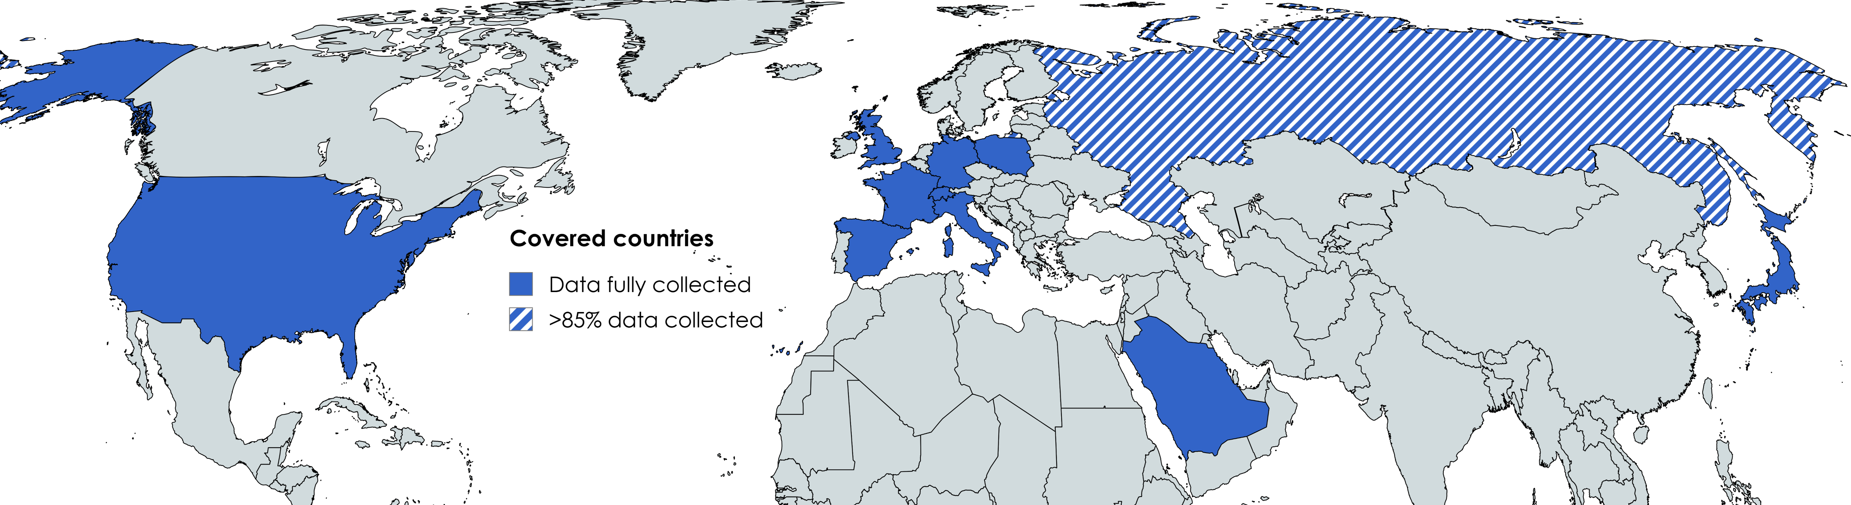
\includegraphics[width=\textwidth]{../figures/maps_participation/country_coverage_progress}}
\bbvs
\ip 11,000/12,000 respondents (Europe: 5,000; USA: 3,000; Japan: 2,000; Saudi Arabia, Russia: 1,000).
\ip Data collected from April 15 to July 3, 2025.
\ip Representative along: gender, age, income, education, urbanicity, region.
\ip Results on control group, weighted using quota variables and country population.
\ip Median duration: 17 min. Inattentive or fast respondents excluded.
\ip Analysis and hypotheses pre-registered.
\ee
\end{frame}

% TODO: intro, literature, representativeness, attrition, biased

% Figures:
% 1? coverage map
% 2. survey_flow
% 3. keywords in fields (taken jointly)
% 4. revenue_split_global+few_global+few_healthcare: one point + error bar for mean per country; one global, one point for # 0% (per country + global)
% 5a. ICS: mean of variant (incl. NCS, GCS) (per country + global) 
% 5b. wealth tax by coverage: mean of variant (country + global)
% 6. conjoint: foreign aid + global tax (per country + global)
% 7. warm_glow: effect of info + display donation vs. control (per country + global)
% 8. solidarity_support (on control): heatmap
% 9. radical_redistr: heatmap sustainability, top_tax, reparations, NCQG?, vote_intl_coalition, group_defended?, my_tax_global_nation, my_tax_global_nation other source?, convergence_support
% 10. group_defended: barresN or barres?
% 11. transfer_how: heatmap (maybe just one row grouping all countries and options in columns)
% 12. average custom_redistr

% Tables:
% 1. ICS: effect of variant (incl. NCS) controlling for GCS_support (per country + global; dans régression avec 2.5 lignes pas répondant, une étant GCS et l'autre NCS) 
% 2. influence of order on split_few_global, on NCQG; of wording on NCQG


% \begin{frame}{Open-ended fields}
% \makebox[\textwidth][c]{ \includegraphics[width=\textwidth]{../figures/country_comparison/}}
% % \bbvs
% % \ip 
% % \ee
% \end{frame}
\begin{frame}{Open-ended fields}
  \bbs \ip Four random branches:
  \bbs \ip \blue{Wishes}: What are your needs or wishes?
 \ip \blue{Issue}: Can you name an issue that is important to you but is neglected in the public debate?
 \ip \blue{Concerns}: What are your main concerns these days?
 \ip \blue{Injustice}: What according to you is the greatest injustice of all?
  \ee
  \ip \textit{Preliminary} findings: 
  \bbs \ip \rose{Main concern}, issue, wish: \rose{purchasing power}.
  \ip Main injustice: poverty.
  \ee
  \ee
\end{frame}

\begin{frame}{Conjoint analysis}
\centering \vspace{.2cm}
\only<+>{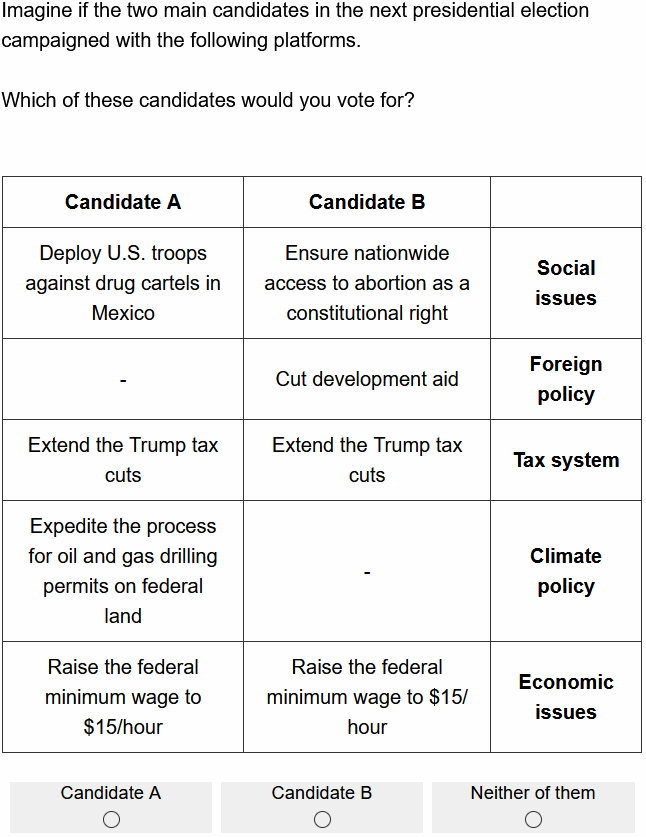
\includegraphics[height=.93\textheight]{../figures/questionnaire/conjoint_US_10.png}}
\only<+>{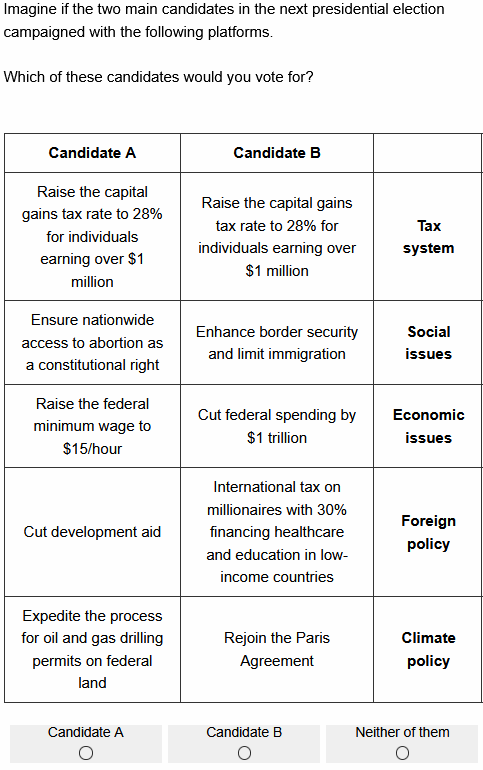
\includegraphics[height=.93\textheight]{../figures/questionnaire/conjoint_US_5.png}}
\only<+>{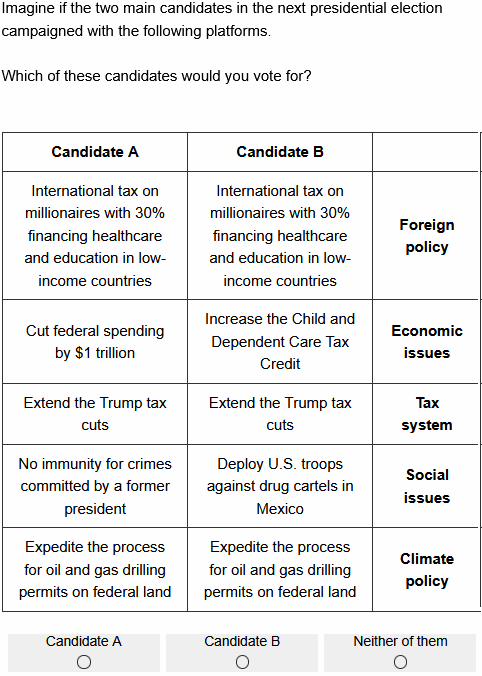
\includegraphics[height=.93\textheight]{../figures/questionnaire/conjoint_US_7.png}}
\only<+>{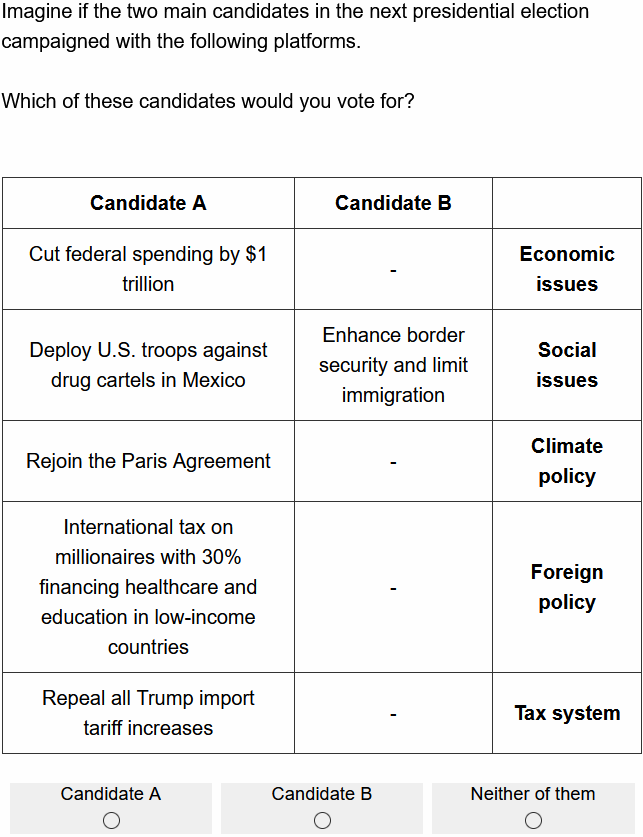
\includegraphics[height=.93\textheight]{../figures/questionnaire/conjoint_US_9.png}}
\only<+>{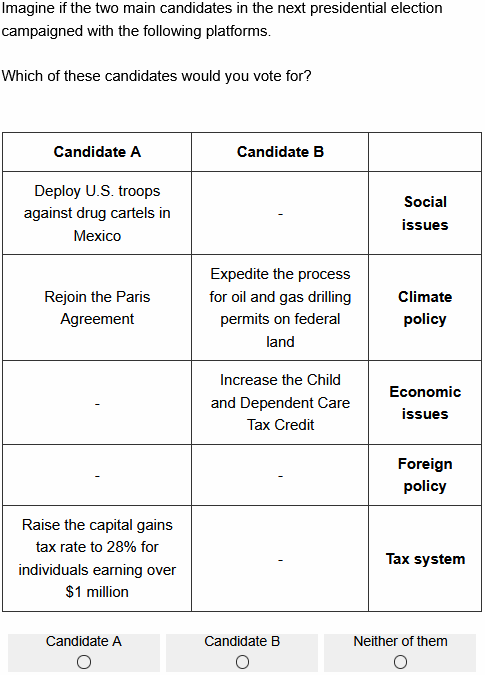
\includegraphics[height=.93\textheight]{../figures/questionnaire/conjoint_US_8.png}} 
\only<+>{}
\only<+>{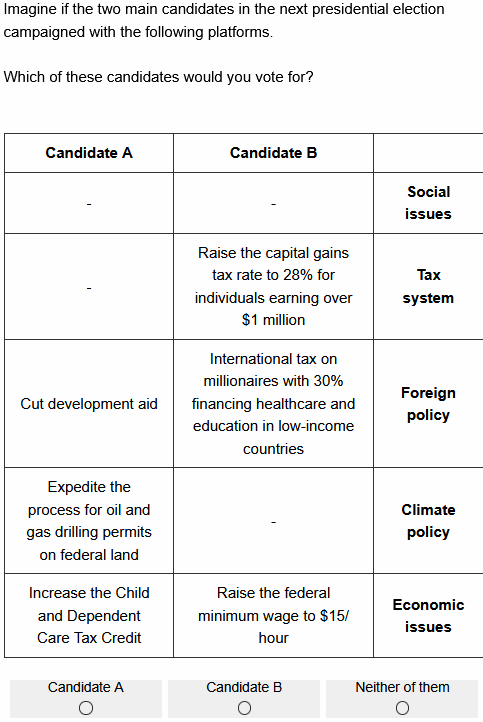
\includegraphics[height=.93\textheight]{../figures/questionnaire/conjoint_US_3.png}} % Cut left
\only<+>{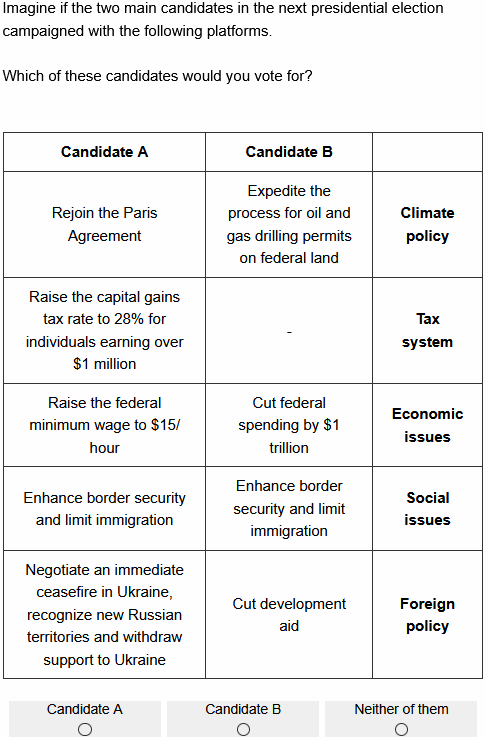
\includegraphics[height=.93\textheight]{../figures/questionnaire/conjoint_US_6.png}} % Cut right
\only<+>{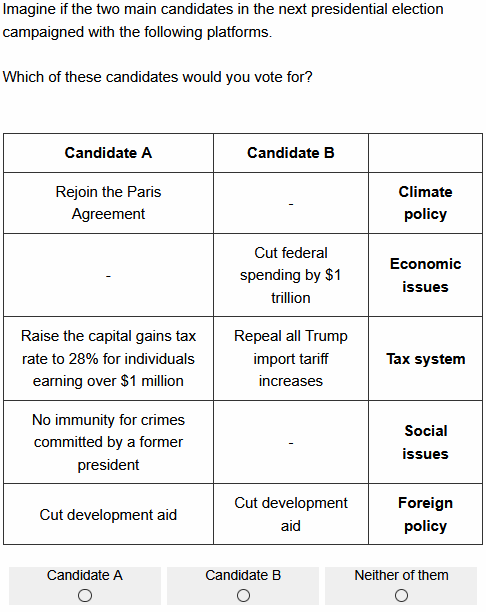
\includegraphics[height=.93\textheight]{../figures/questionnaire/conjoint_US_2.png}} % Cut in both
\only<+>{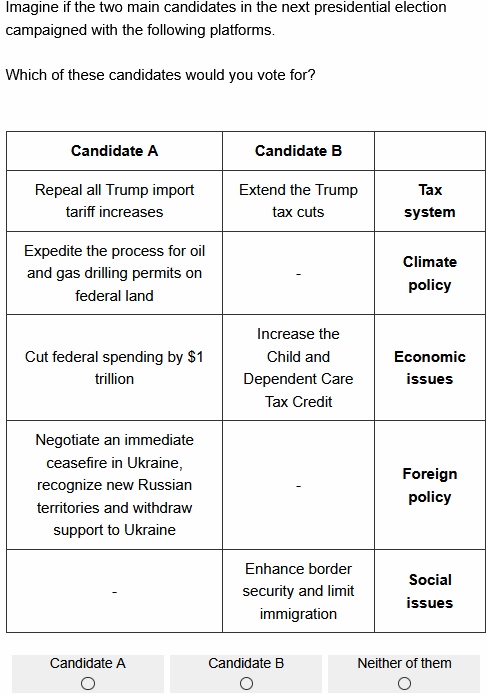
\includegraphics[height=.93\textheight]{../figures/questionnaire/conjoint_US_1.png}} % Cut in none
\end{frame}

\begin{frame}{Conjoint analysis\label{conjoint_country}} 
    \begin{figure}
\caption{Conjoint analysis in Germany (Average Marginal Component Effect) \hyperlink{conjoint_countries}{\beamergotobutton{Other countries}}} 
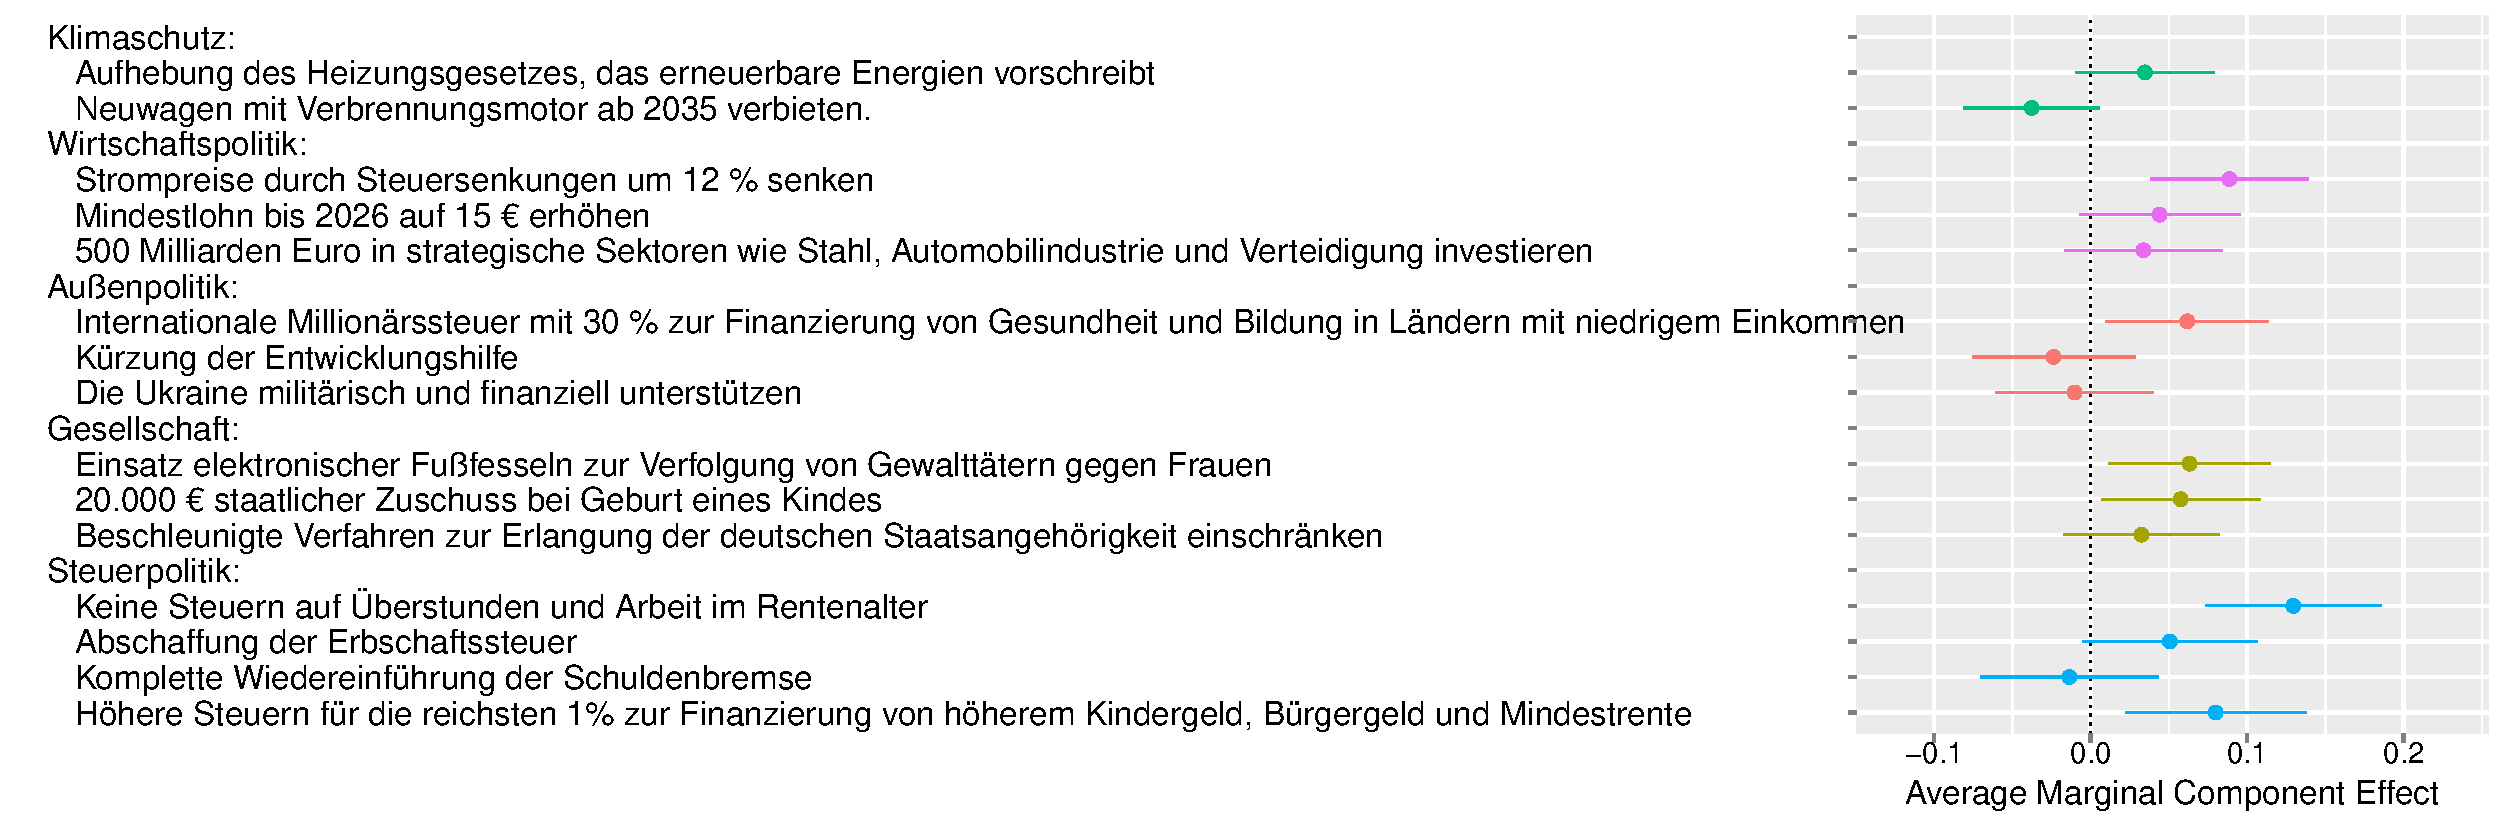
\includegraphics[width=\textwidth]{../figures/DE/conjoint_DE.pdf}
\end{figure}
\end{frame}

\begin{frame}{Conjoint analysis} 
    \begin{figure}
\caption{\rose{Effect on} the \rose{likelihood that a} political \rose{program is preferred} of containing the following policy%\\(compared to no foreign policy in the program):
} \vspace{-.3cm}
\begin{subfigure}{.48\textwidth}
  \caption[]{\blue{Cut development aid}: $-$5 pp*** \quad \green{\checkmark H1a}}\vspace{-.3cm}
  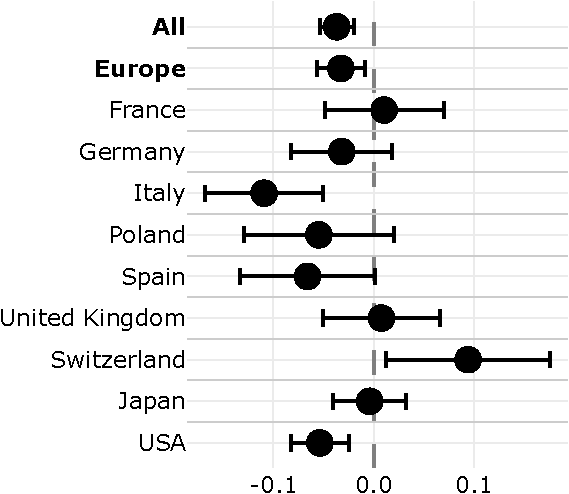
\includegraphics[width=\textwidth]{../figures/country_comparison/program_preferred_by_cut_aid_in_program.pdf}
\end{subfigure} \pause
\begin{subfigure}{.50\textwidth}
  \caption[]{\blue{International tax on millionaires with 30\% financing} health and education in \blue{low-income countries}: +5 pp*** \quad \green{\checkmark H1b}} \vspace{-.3cm}
  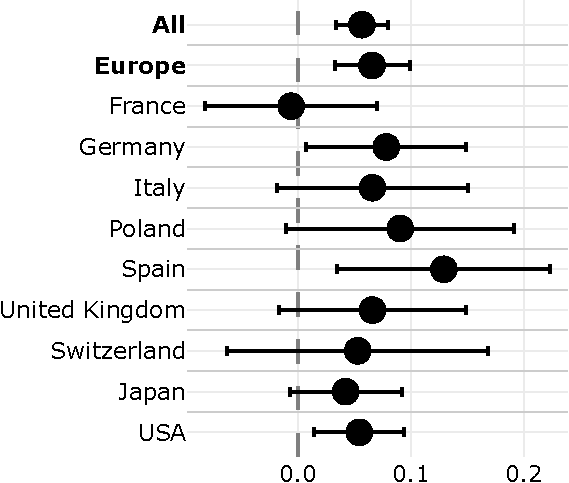
\includegraphics[width=.95\textwidth]{../figures/country_comparison/program_preferred_by_millionaire_tax_in_program.pdf}
\end{subfigure}
\end{figure}
\end{frame}

\begin{frame}{Revenue split}
\centering How should revenue from a global tax on millionaires be allocated? (in \%) \quad \green{\checkmark H2}
\only<+>{\makebox[\textwidth][c]{
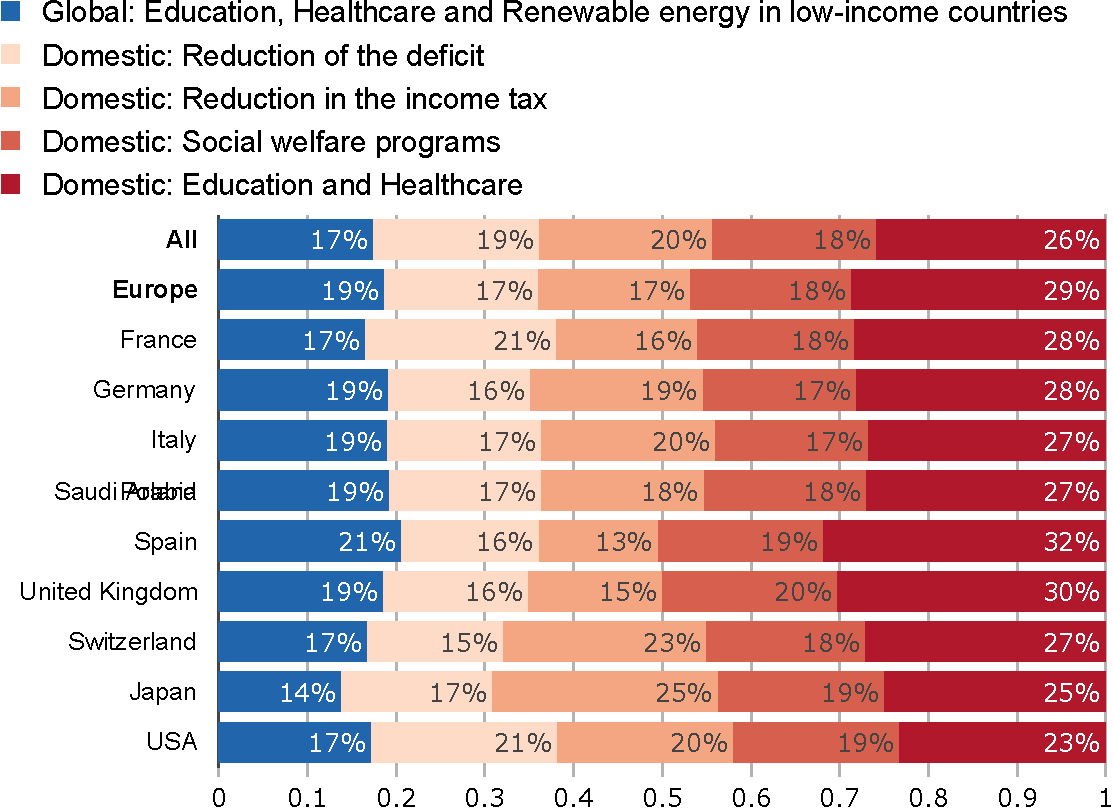
\includegraphics[width=\textwidth]{../figures/country_comparison/split_few_bars.pdf}}}
\only<+>{\makebox[\textwidth][c]{
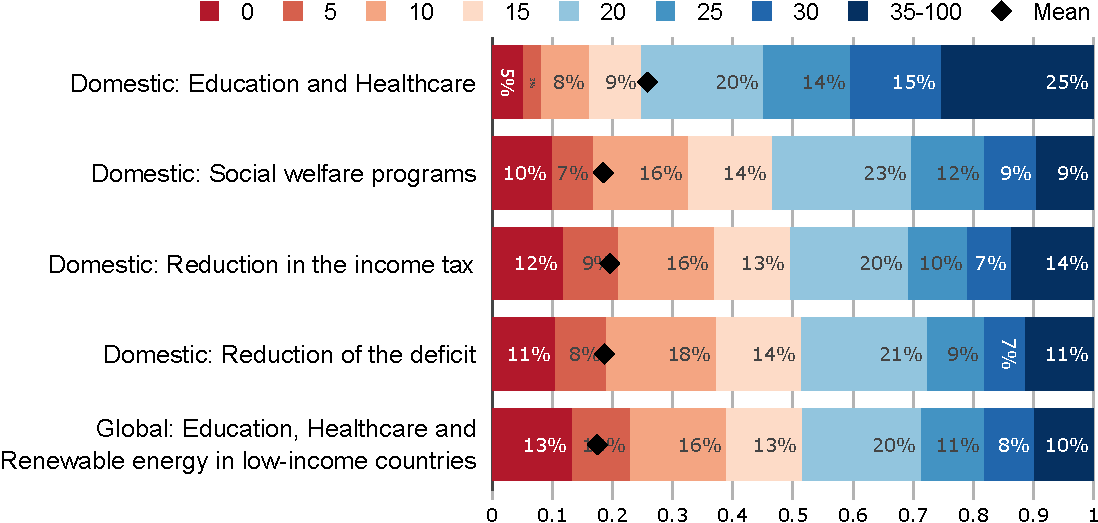
\includegraphics[width=\textwidth]{../figures/all/split_few.pdf}}}
\end{frame}

\begin{frame}{International wealth tax}
\centering Support for a 2\% wealth tax above [\$1 million] with 30\% financing public services in LICs,\\depending on which countries adopt it(random variant).
%     {\centering Imagine an international tax on individuals with net worth above [wealth_threshold: \$1 million]. \\
% Only wealth above [wealth_threshold: \$1 million] would be taxed, at a rate of 2\%. Each country would retain 70\% of the revenues it collects, while 30\% would be pooled at the global level to finance public services in low-income countries (in particular, access to drinking water, healthcare, and education in Africa). \\
% \\
% Say we are in 2030. [International: Imagine that some countries  (such as the European Union) adopt this policy and others (such as Japan, Canada, and China) do not.]\\
% Do you support [country_name: the United States] adopting this international tax on millionaires? }
\makebox[\textwidth][c]{ 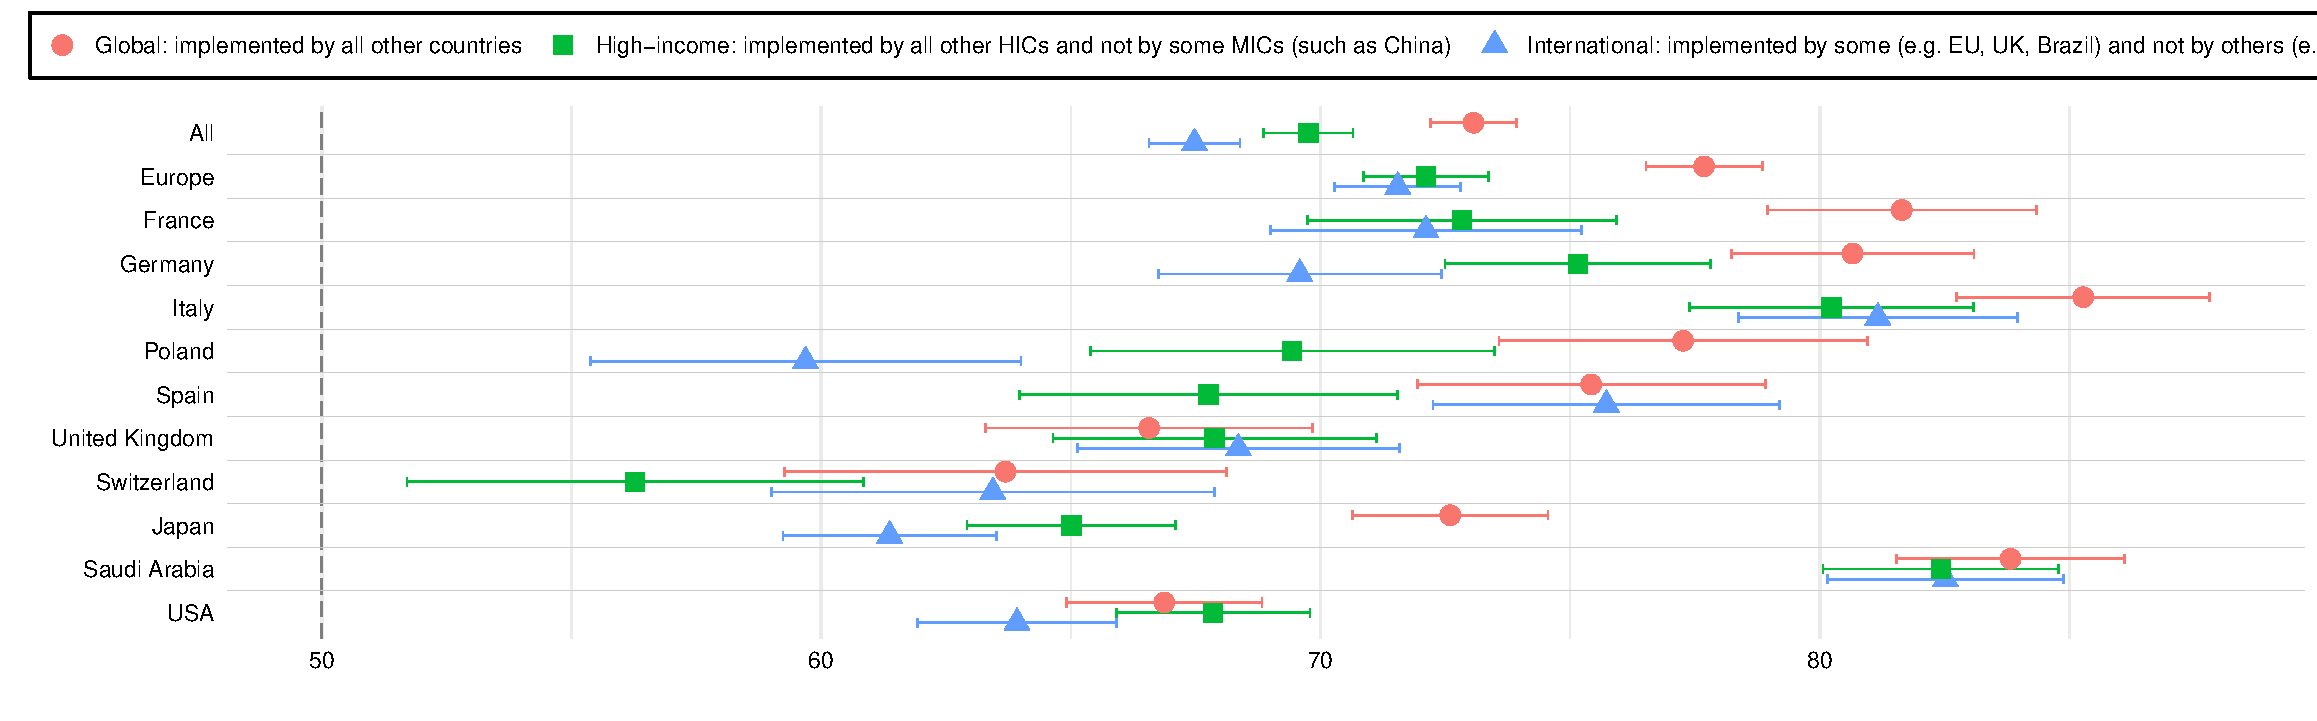
\includegraphics[width=\textwidth]{../figures/country_comparison/variables_wealth_tax_support_by_country}} % wealth_tax_support_positive
% \bbvs
% \ip 
% \ee
\end{frame}

\begin{frame}{Climate Scheme\label{cs}} 
    \bbvsp \ip 3 random branches:
      \bbvsp \ip Donation experiment: \textit{In case you win the lottery, what share of the \$100 would you donate to plant trees?}
      \ip National Climate Scheme (NCS): a cap-and-trade financing equal cash transfers.
      \ip Control group: $\varnothing$. \ee
    \ip Global Climate Scheme (GCS): \hyperlink{gcs_question}{\beamergotobutton{Question text}} 
      \bbvsp \ip Description incentivized for comprehension (73\% get it right).
      \ip A \textit{global} cap-and-trade financing a \textit{global} basic income of [\$35]/month.
      \ip Salient cost: ``\textbf{The typical [country] person would lose out financially [U.S.: \$90, UK: £20...] per month} (as he or she would face around [U.S.: 2, UK: 1]\% in price increases, which is higher than the [\$35] per month they would receive).'' \ee
    \ip Belief of support for the GCS. 2 random branches:
      \bbvs \ip In own country.
      \ip In the U.S. \ee
    \ip International Climate Scheme (GCS where country participation is specified). 4 random branches:
    \bbvs \ip  Country coverage variants: \textit{Low}; \textit{Mid}; \textit{High}; \textit{High color} (color: visible distributive effects). \ee
    \ee
\end{frame}

\begin{frame}{Majority support for the GCS and pluralistic ignorance}
\makebox[\textwidth][c]{ 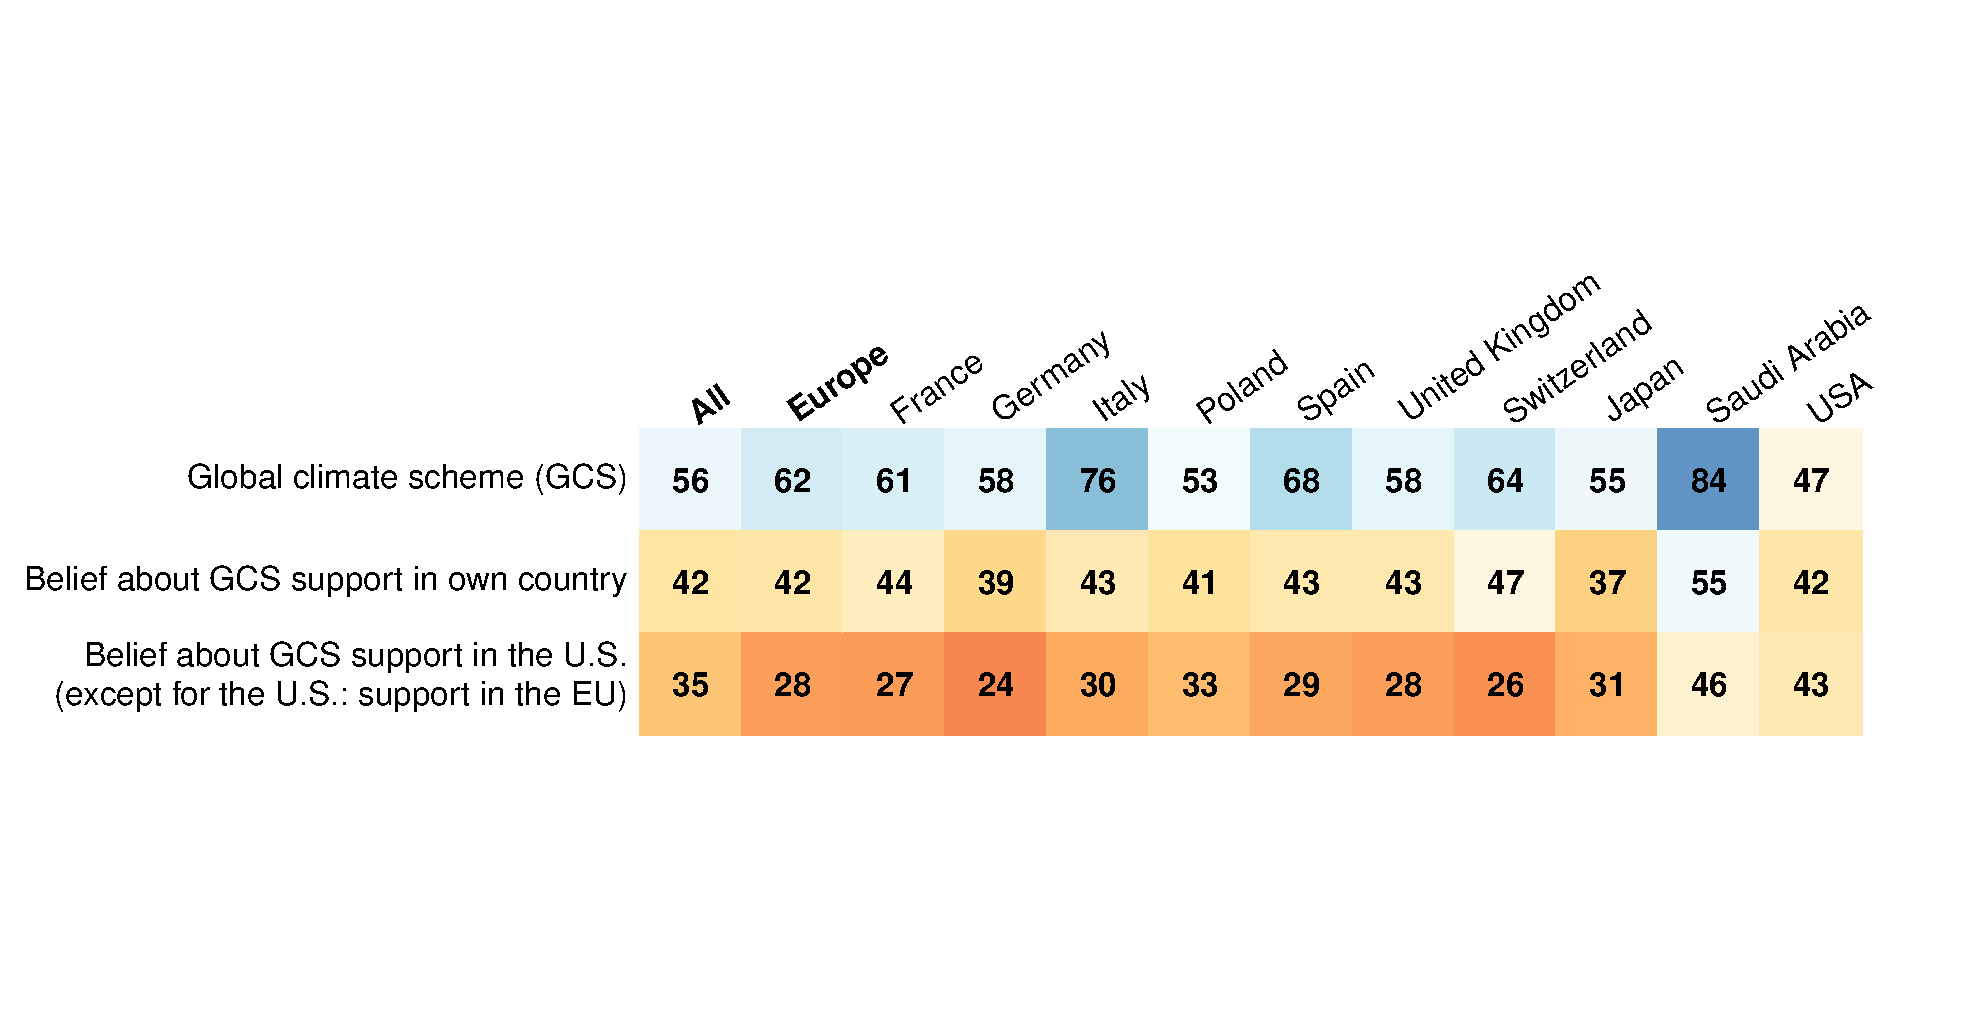
\includegraphics[width=\textwidth]{../figures/country_comparison/gcs_belief_mean.pdf}} 
% \ee
\end{frame}

\begin{frame}{International Climate Scheme}
    \centering 
\only<+>{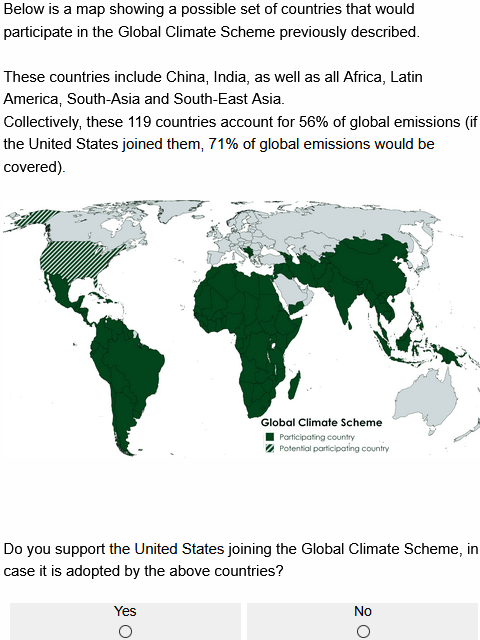
\includegraphics[height=.93\textheight]{../figures/questionnaire/survey_ics_mid.png}} 
\only<+>{\centering \blue{\textbf{Low}}: Global South + EU (25-33\% of world emissions)
  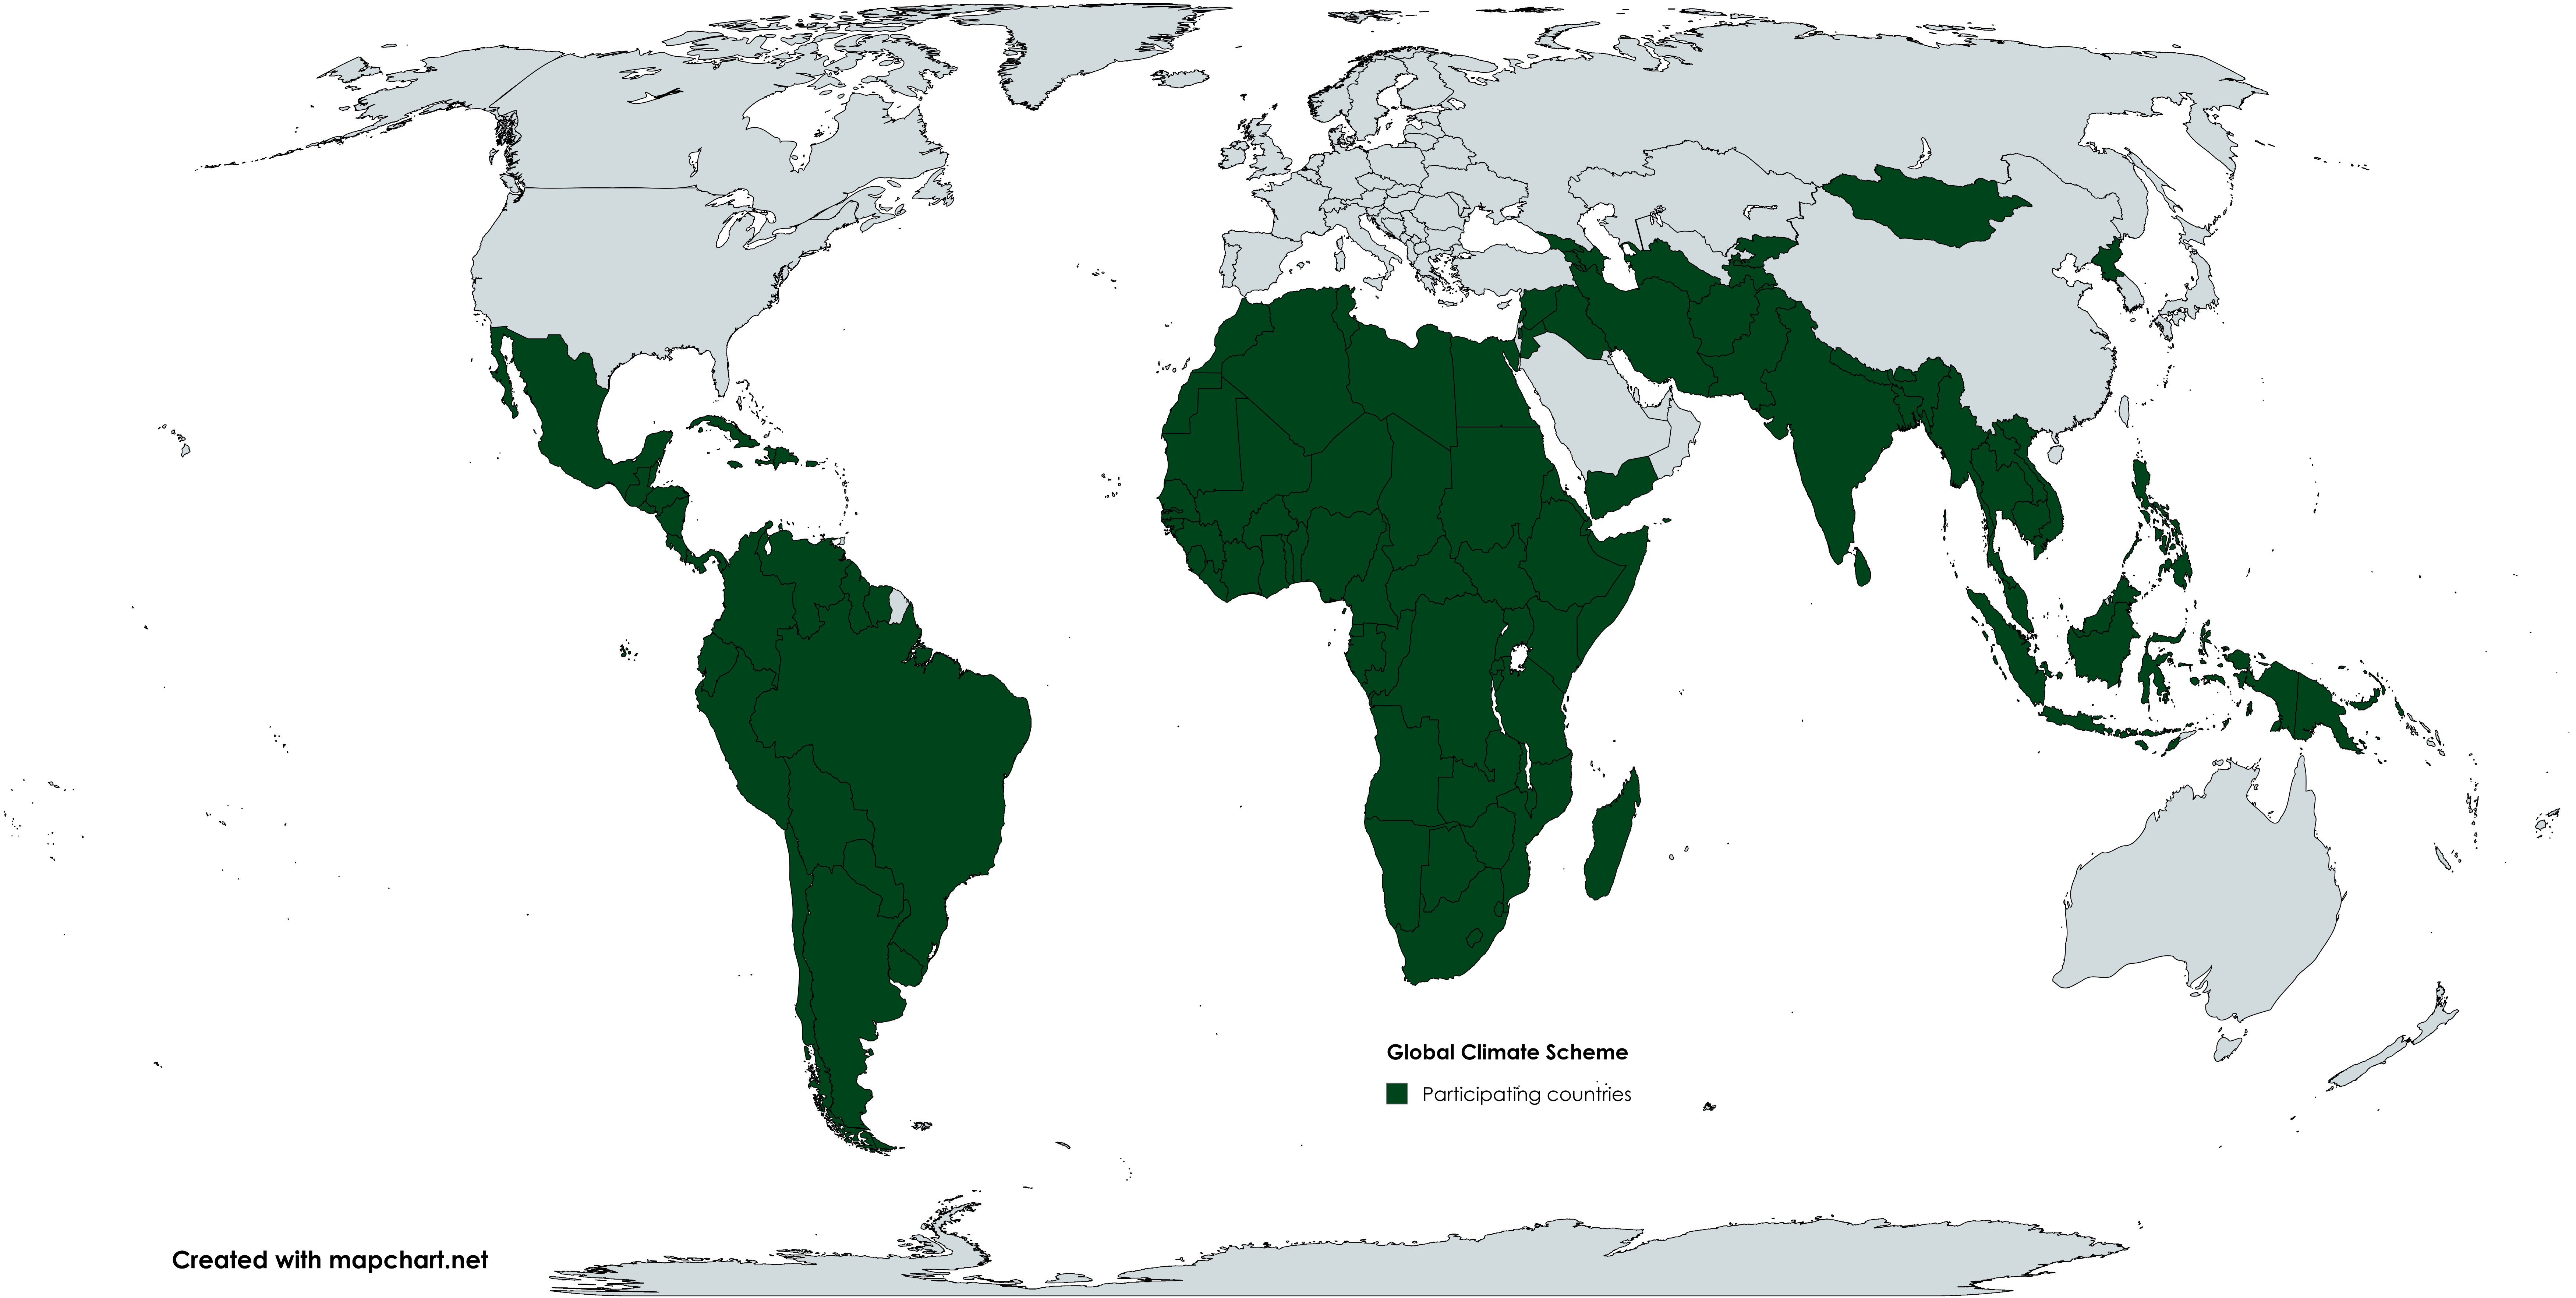
\includegraphics[height=.85\textheight]{../figures/maps_participation/GCS_low.png}} 
\only<+>{\centering \blue{\textbf{Mid}} coverage: Global South + China (56\% of world emissions)
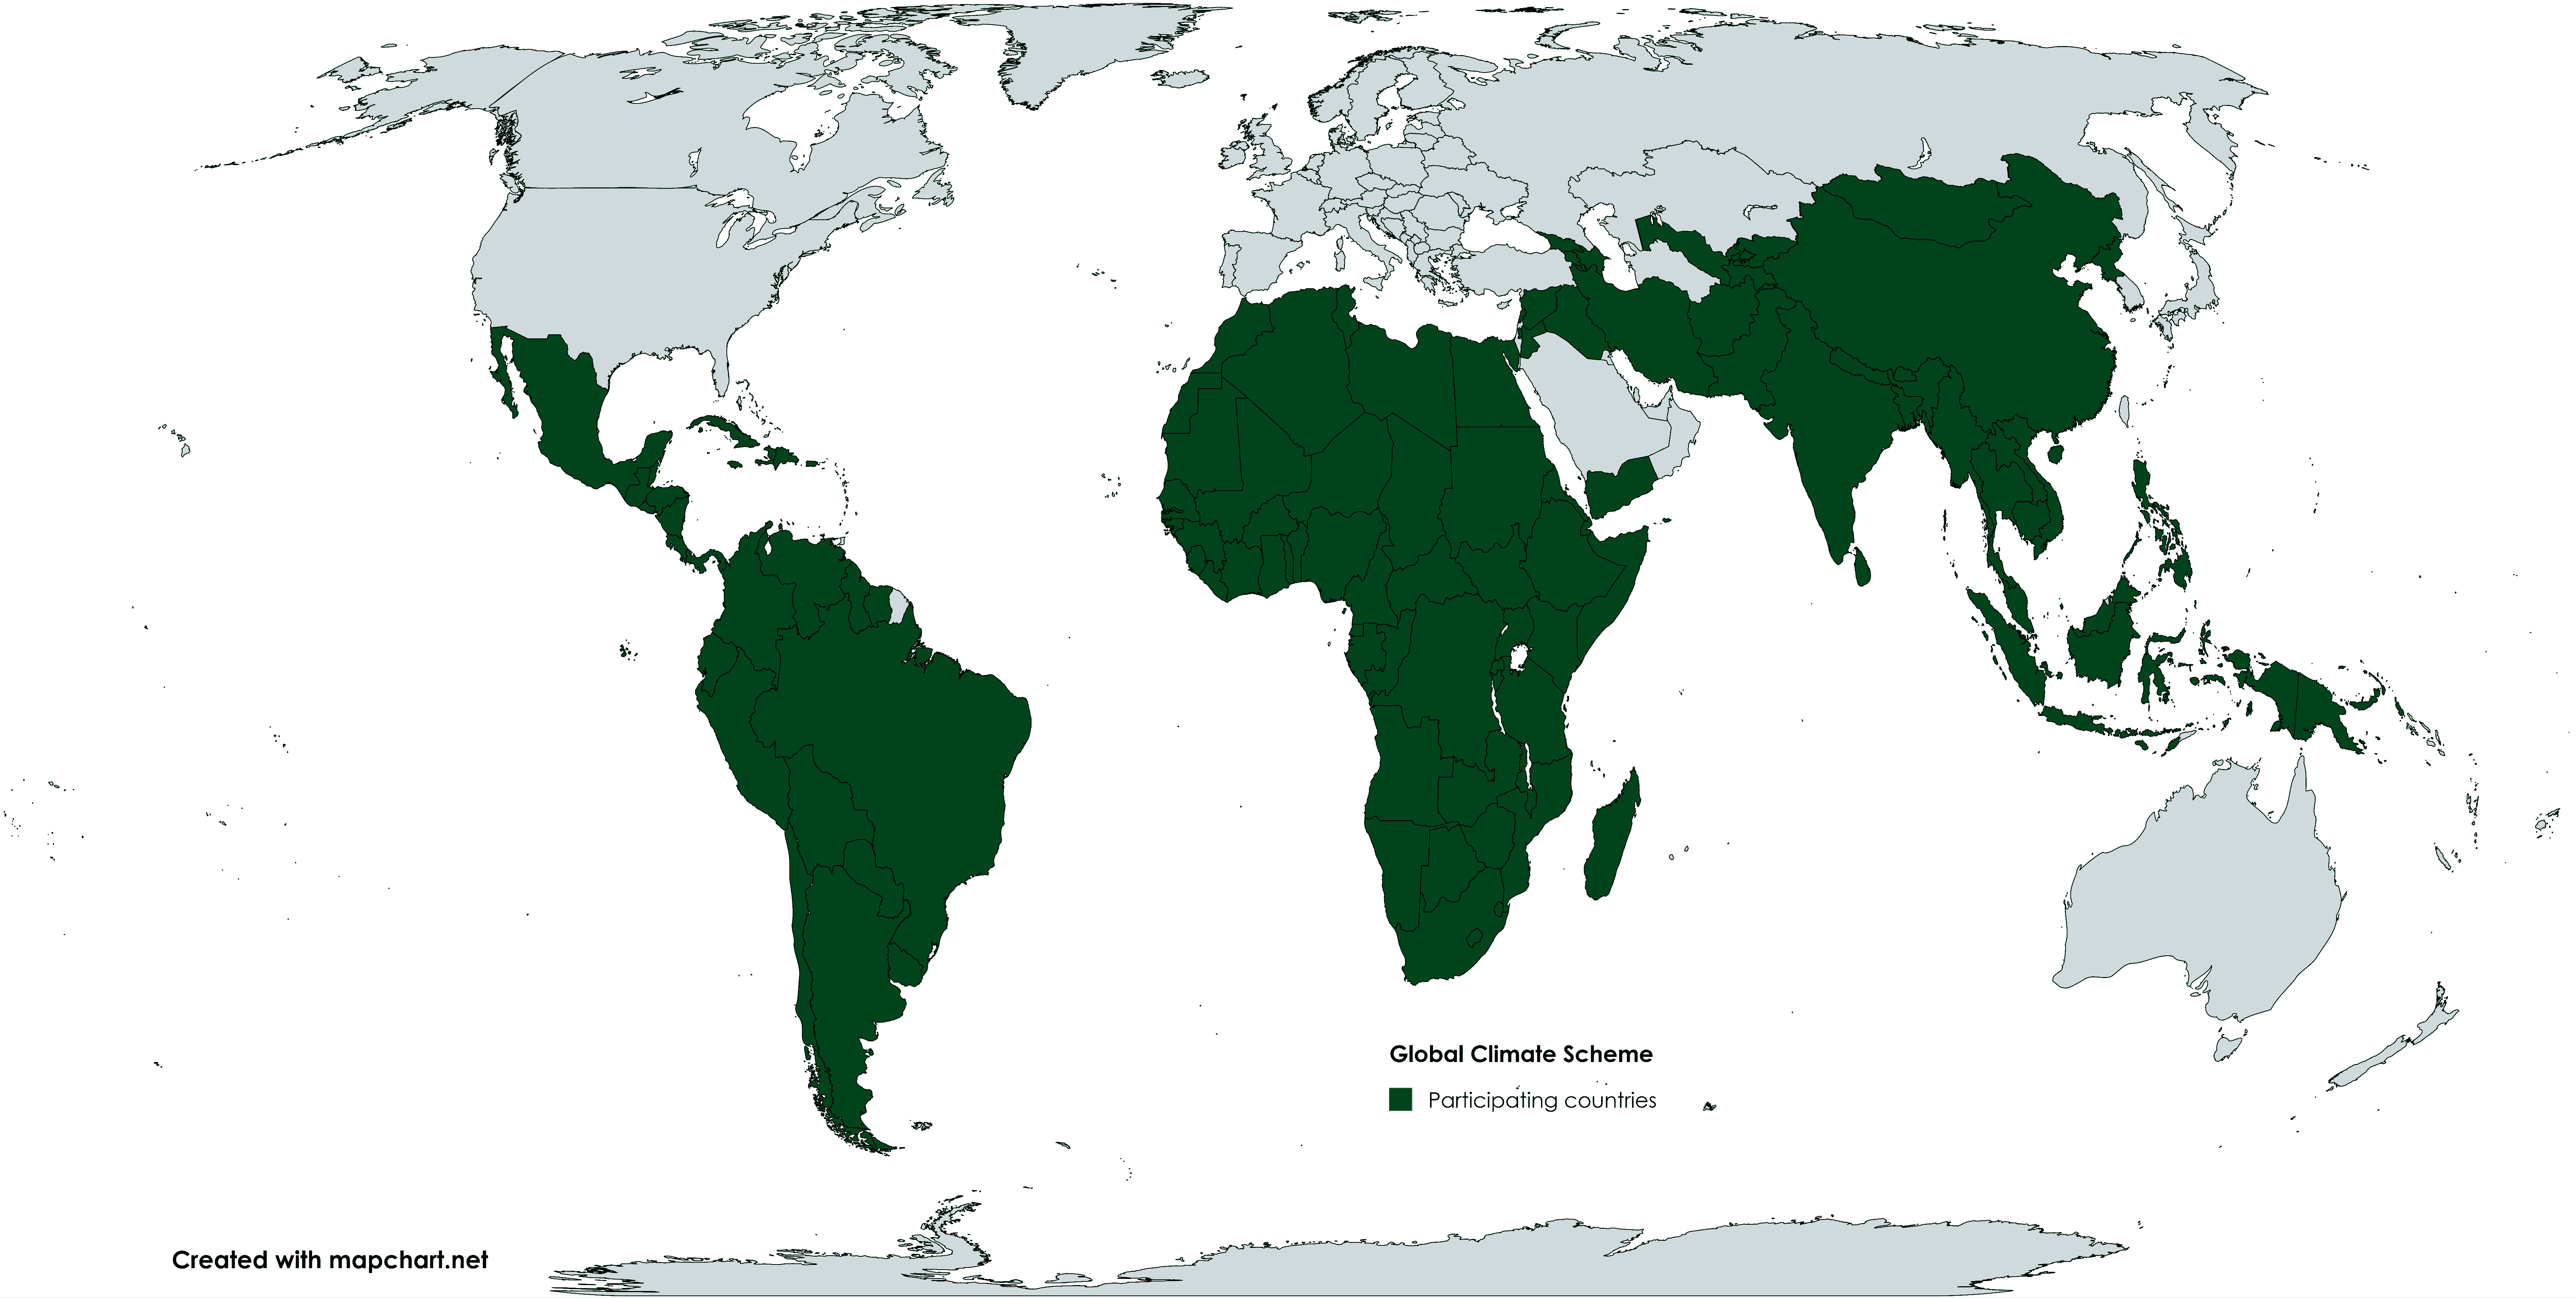
\includegraphics[height=.85\textheight]{../figures/maps_participation/GCS_mid.png}}
\only<+>{\centering \blue{\textbf{High}} coverage: Global South + China + EU + various HICs (64-72\% of world emissions)
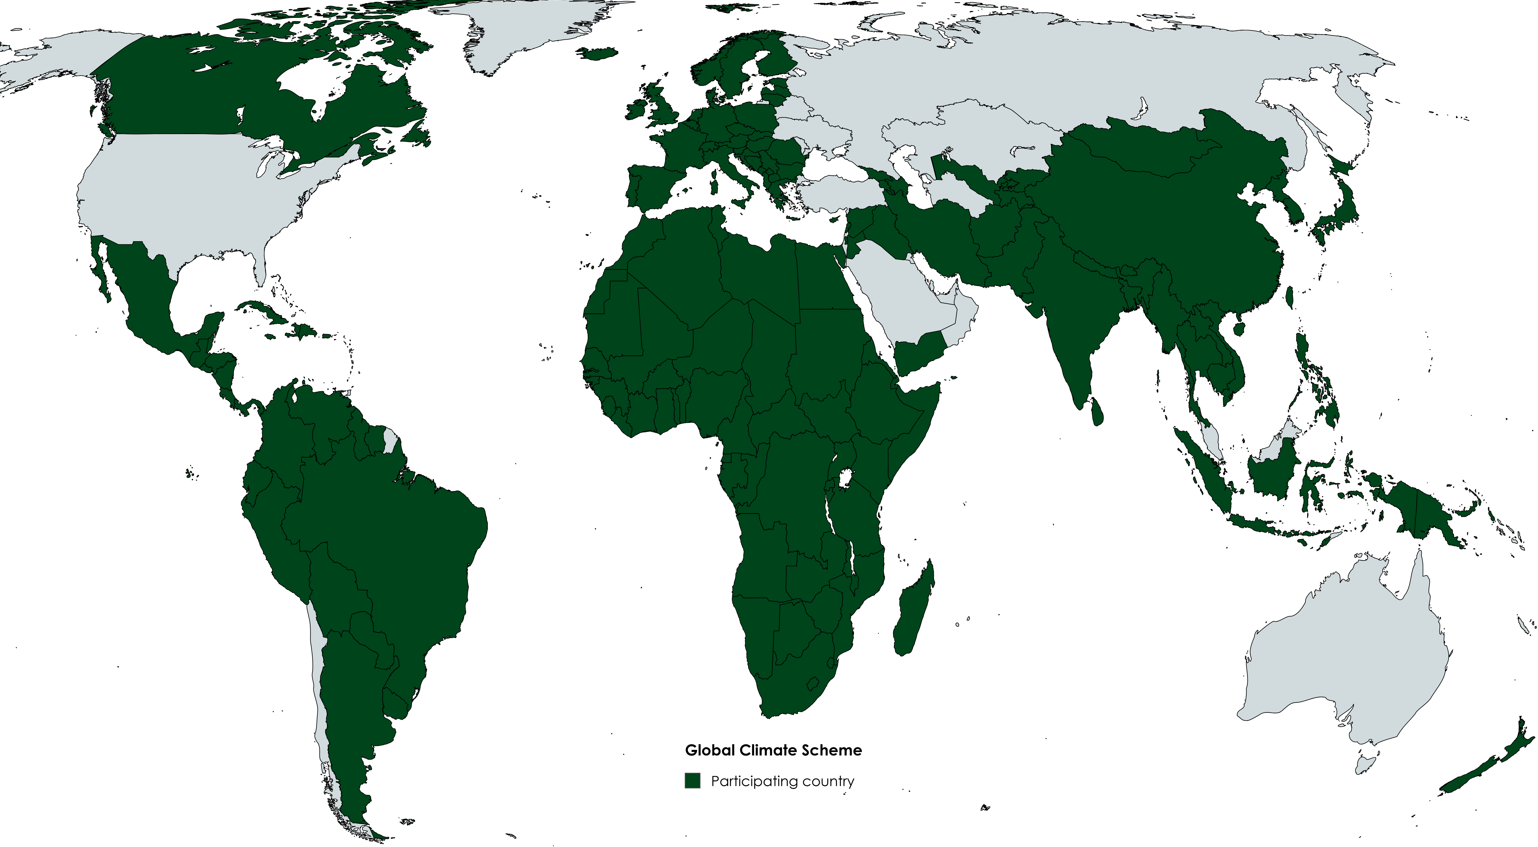
\includegraphics[height=.85\textheight]{../figures/maps_participation/GCS_high.png}}
\only<+>{\centering \blue{\textbf{High}} coverage (64-72\% of world emissions), \rose{\textbf{color}} variant
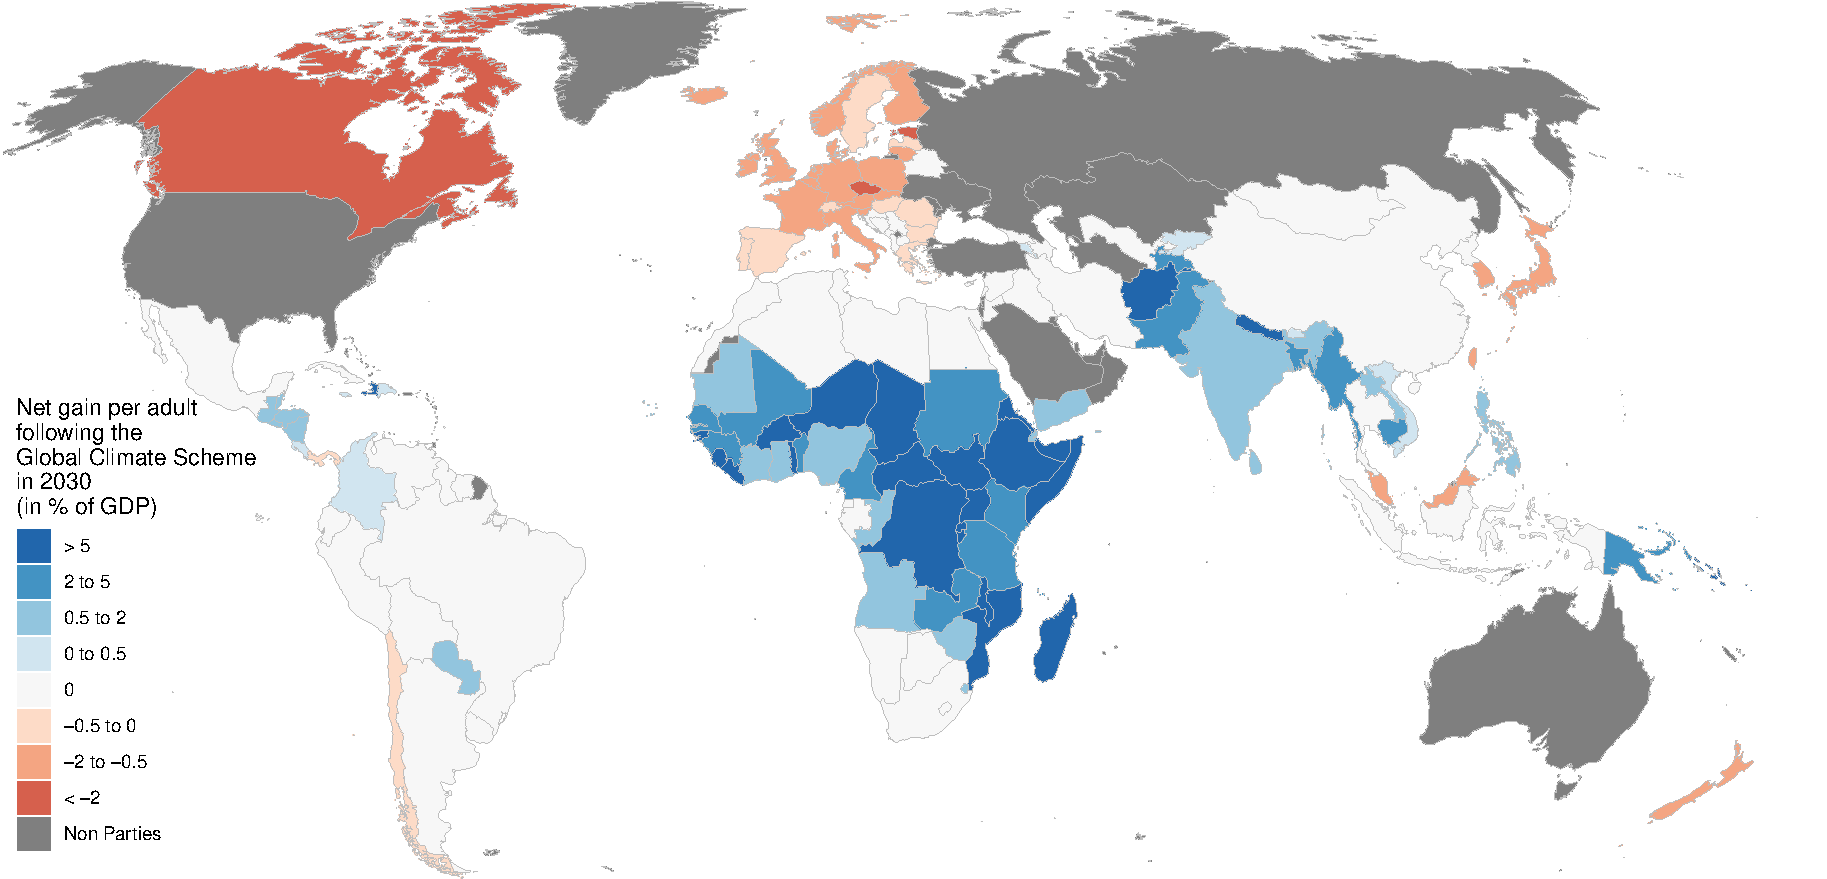
\includegraphics[height=.85\textheight]{../figures/maps_participation/GCS_high_color.pdf}}
\only<+>{\centering \textbf{High color} as shown in the U.S.
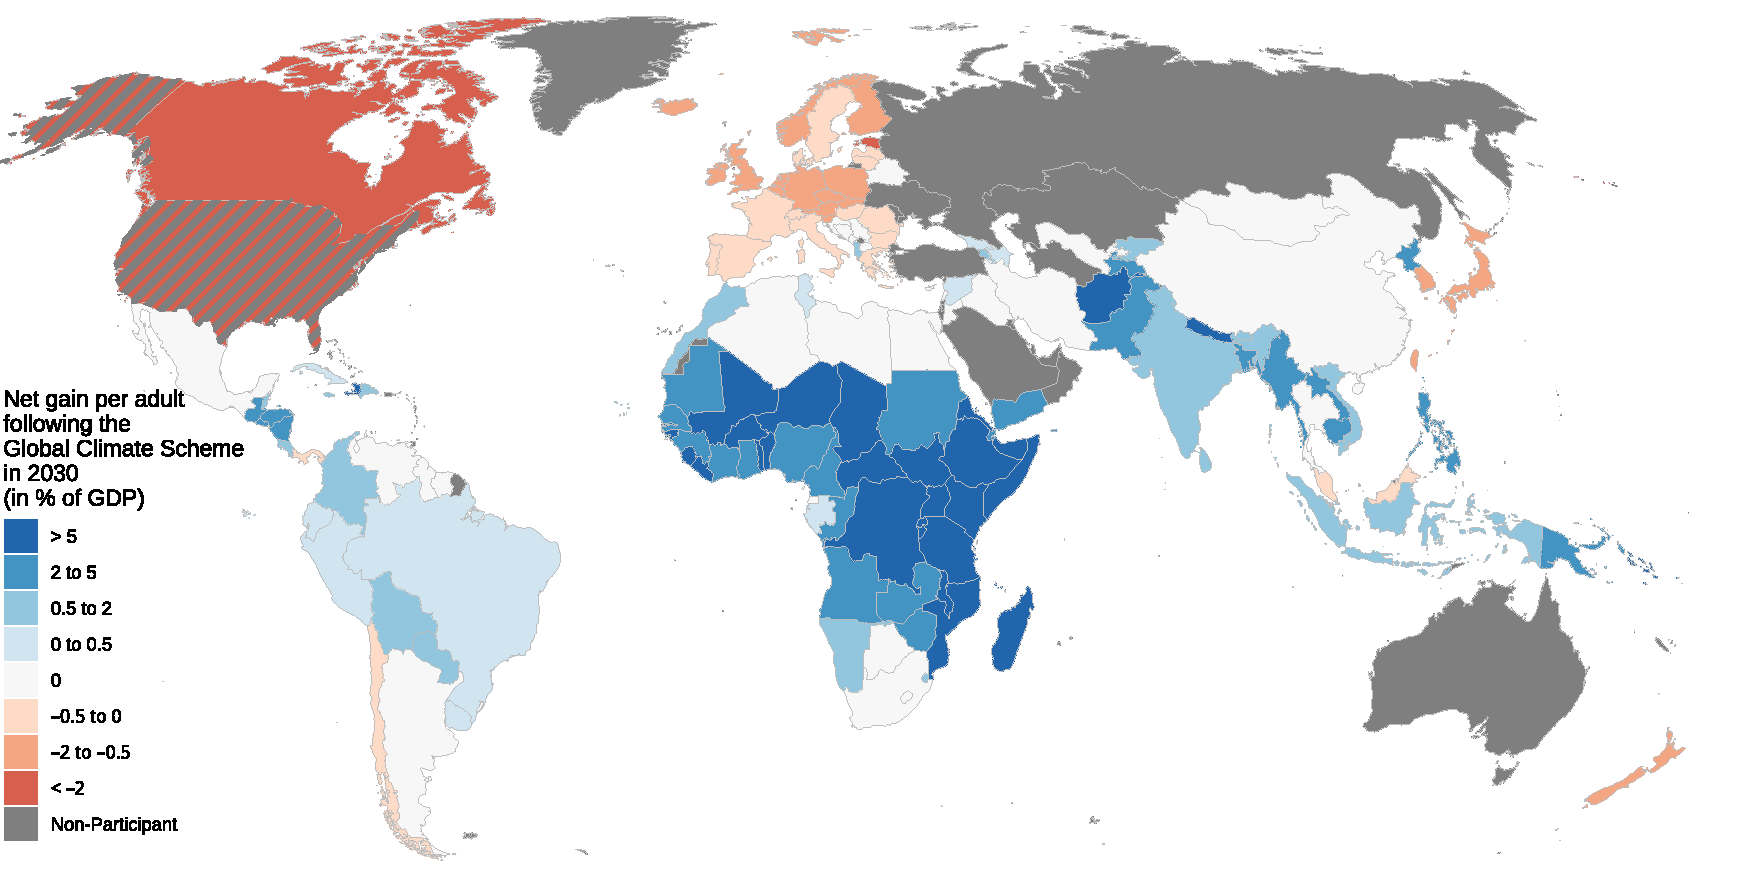
\includegraphics[height=.85\textheight]{../figures/maps_participation/GCS_high_color_EN.pdf}}
\only<+>{\centering \textbf{High color} as shown in France
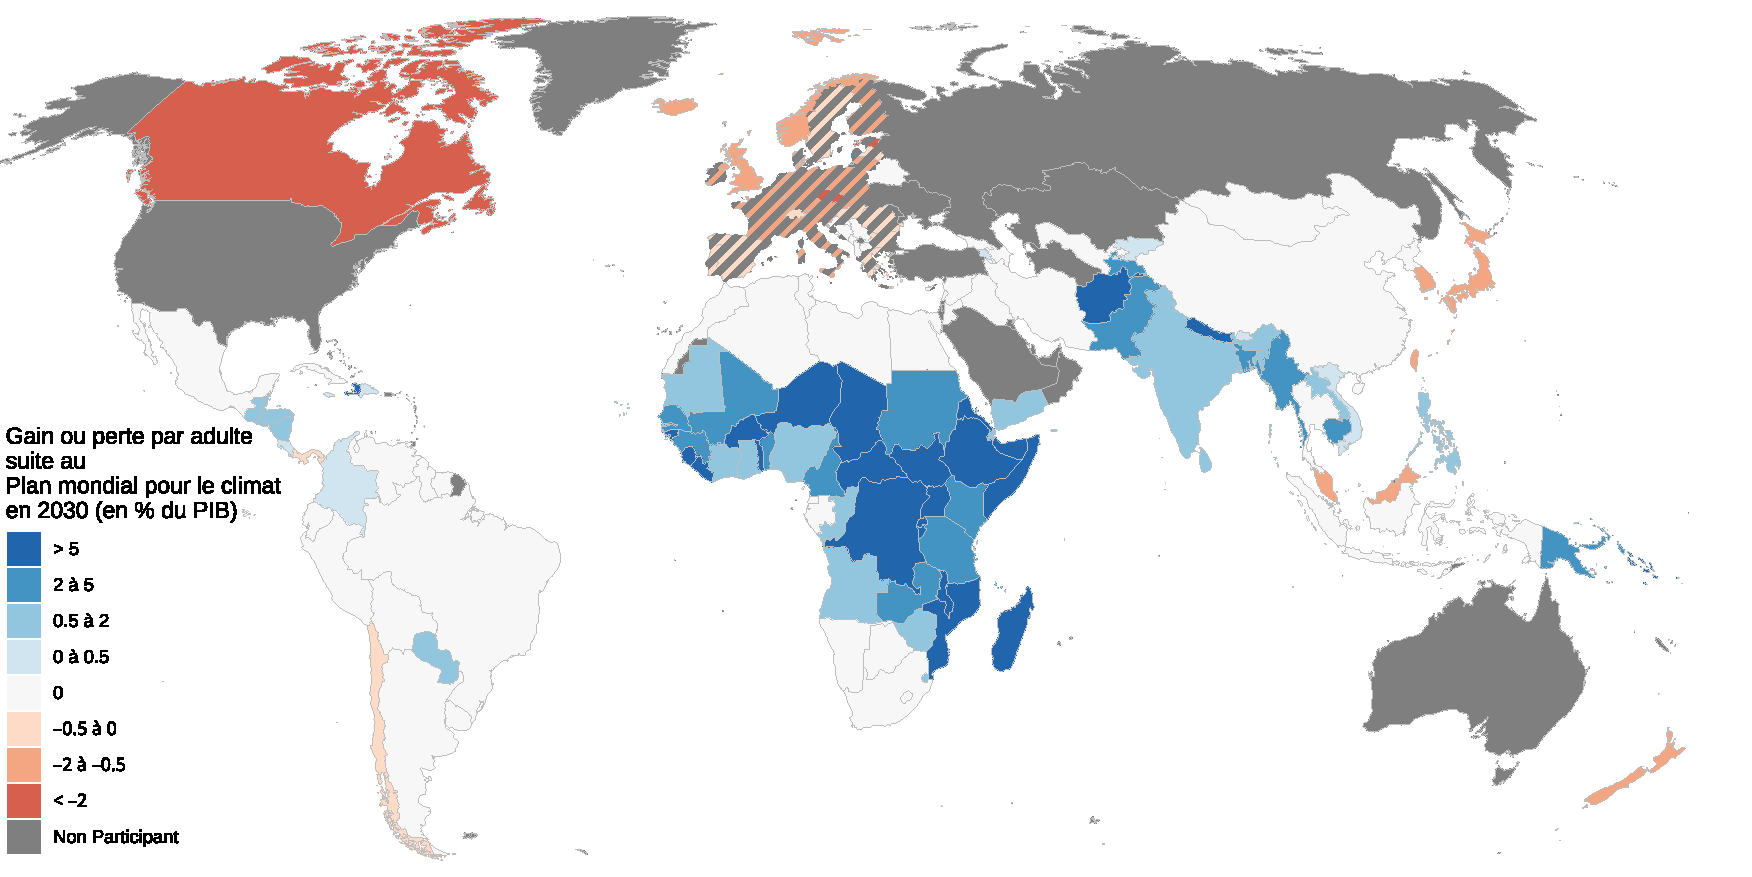
\includegraphics[height=.85\textheight]{../figures/maps_participation/GCS_high_color_FR.pdf}}
\only<+>{\centering \textbf{High color} as shown in Saudi Arabia
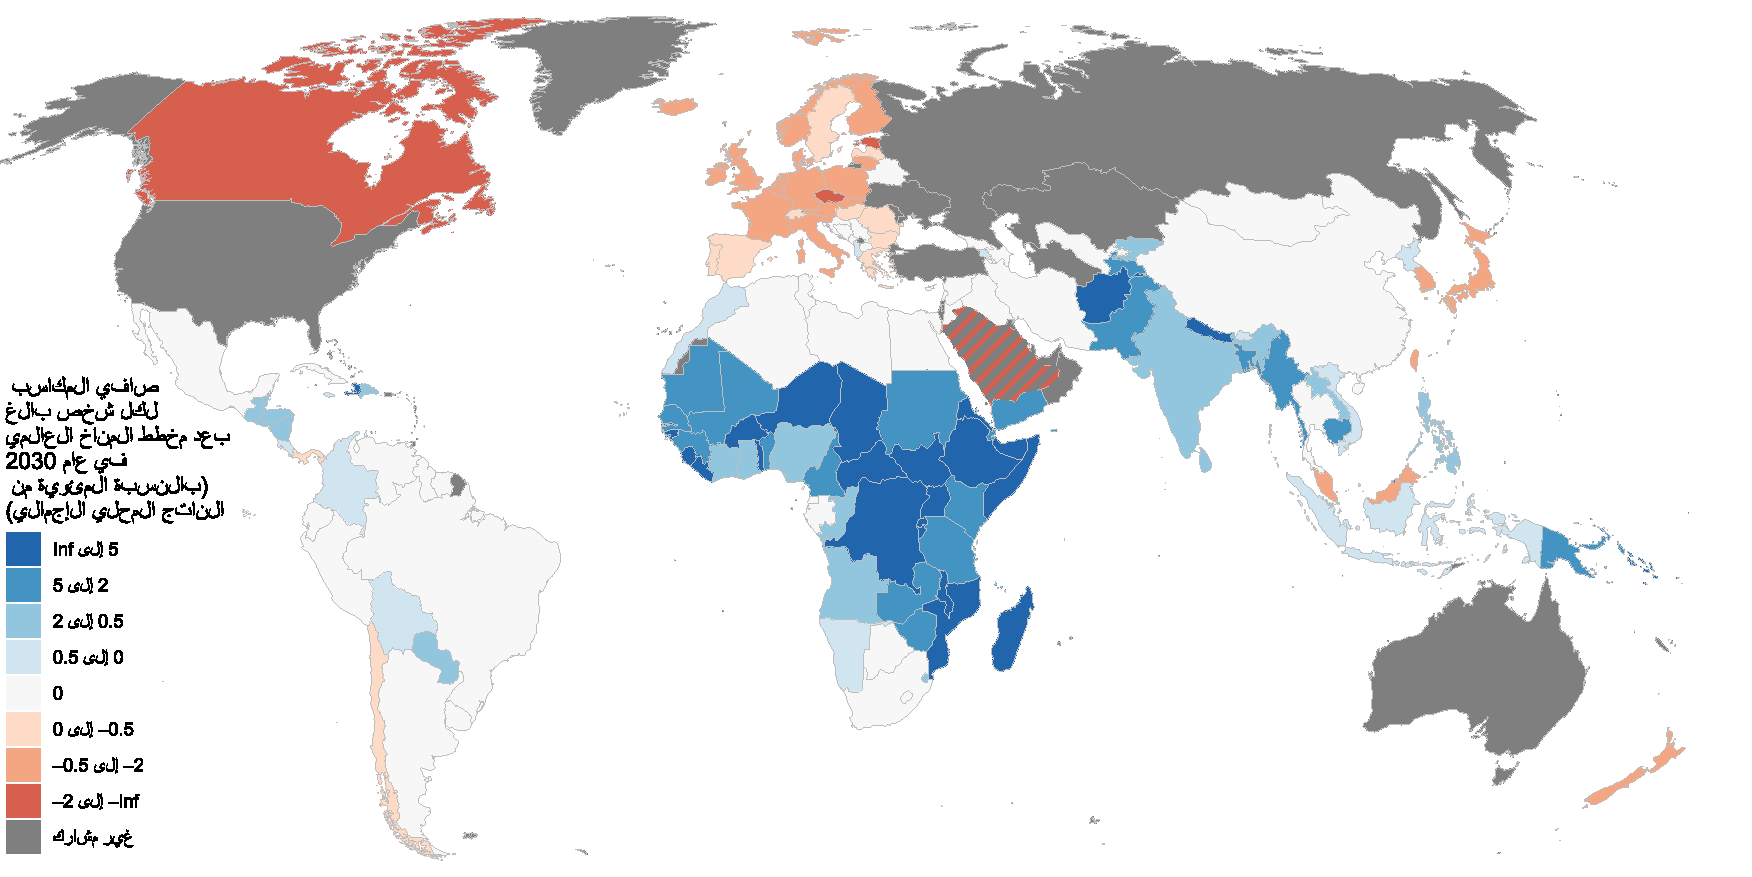
\includegraphics[height=.85\textheight]{../figures/maps_participation/GCS_high_color_AR.pdf}}
\end{frame}

\begin{frame}{International Climate Scheme}
\makebox[\textwidth][c]{ 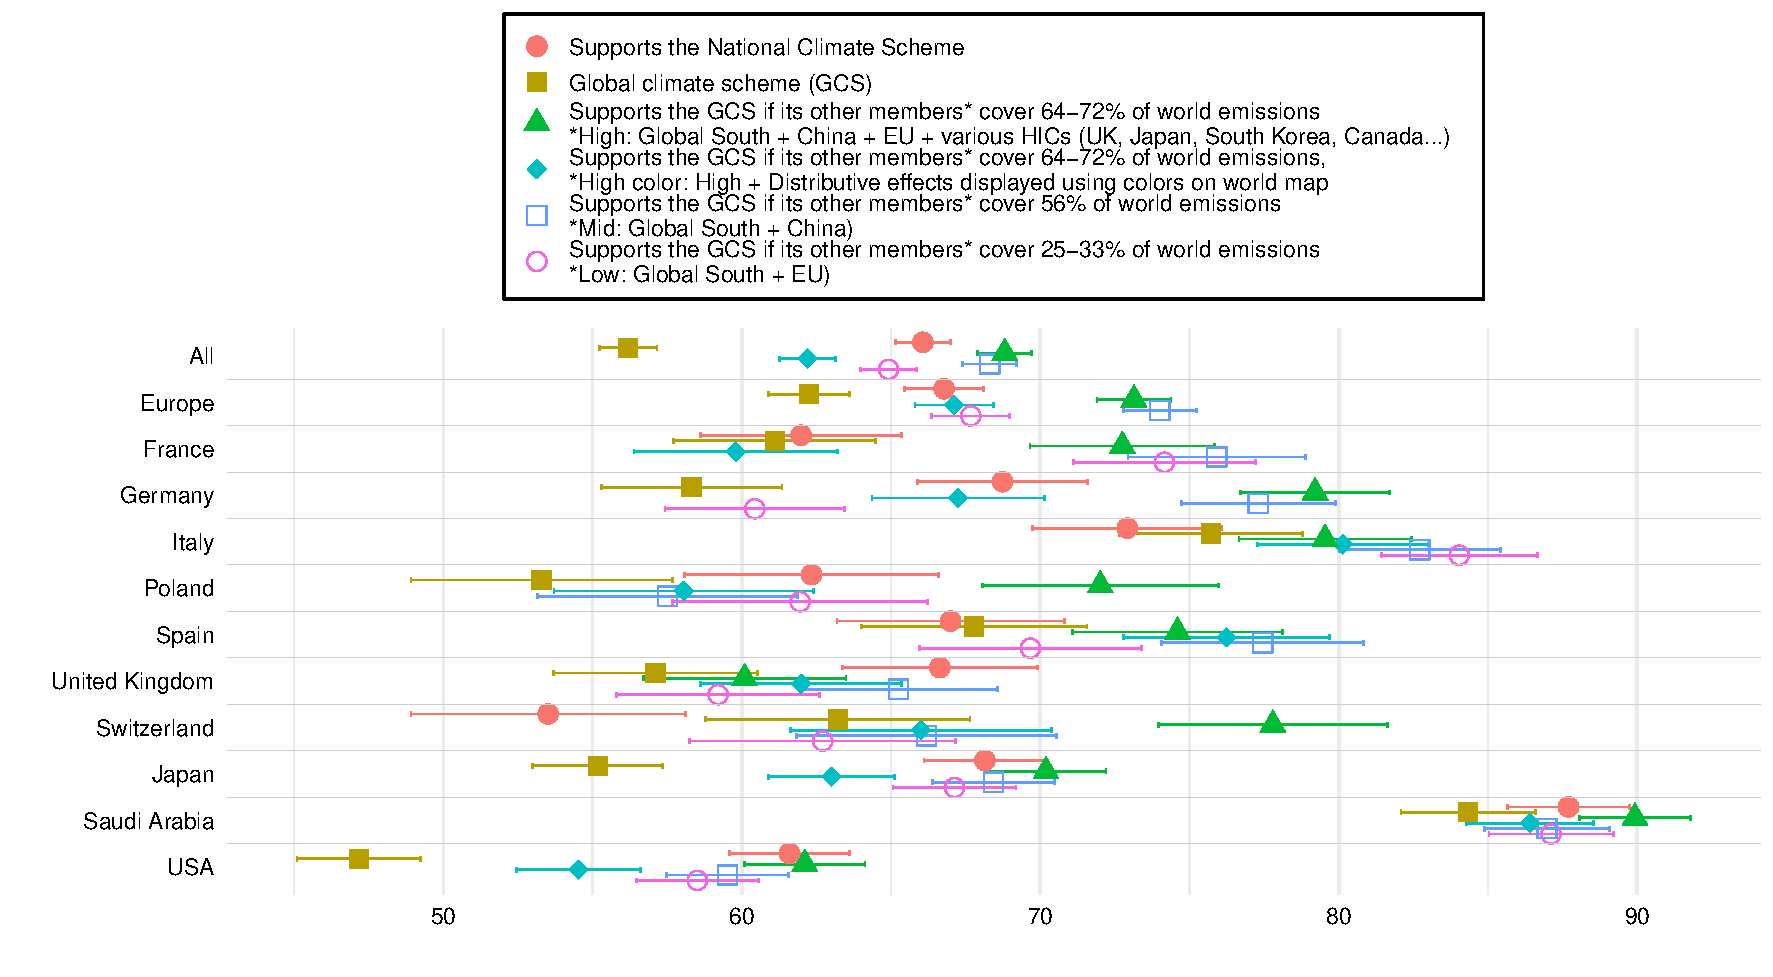
\includegraphics[width=\textwidth]{../figures/country_comparison/variables_ncs_gcs_ics_by_country}} % ncs_gcs_ics_all_mean
\bbvsp
% (Bechtel and Scheve 2013; Carlsson et al. 2013; Dabla-Norris et al. 2023; Gampfer, Bernauer, and Kachi 2014)
\ip \rose{Majority support} for all variants in all countries when participation map is shown. \quad \green{\checkmark H4a}
\ip \blue{+4 p.p.} when coverage expanded from \blue{Low} to \blue{High}. \quad \green{\checkmark H4b}
\ip \rose{$-$6 p.p. when distributive effects are visible}.
\ee
\end{frame}

\begin{frame}{Plausible gobal policies\label{solidarity_support_relative}}
\centering Share of (somewhat or strong) \textit{support} among non-\textit{indifferent} answers. \quad \green{\checkmark H3} \hyperlink{solidarity_support_absolute}{\beamergotobutton{Absolute support}} \\
\makebox[\textwidth][c]{ 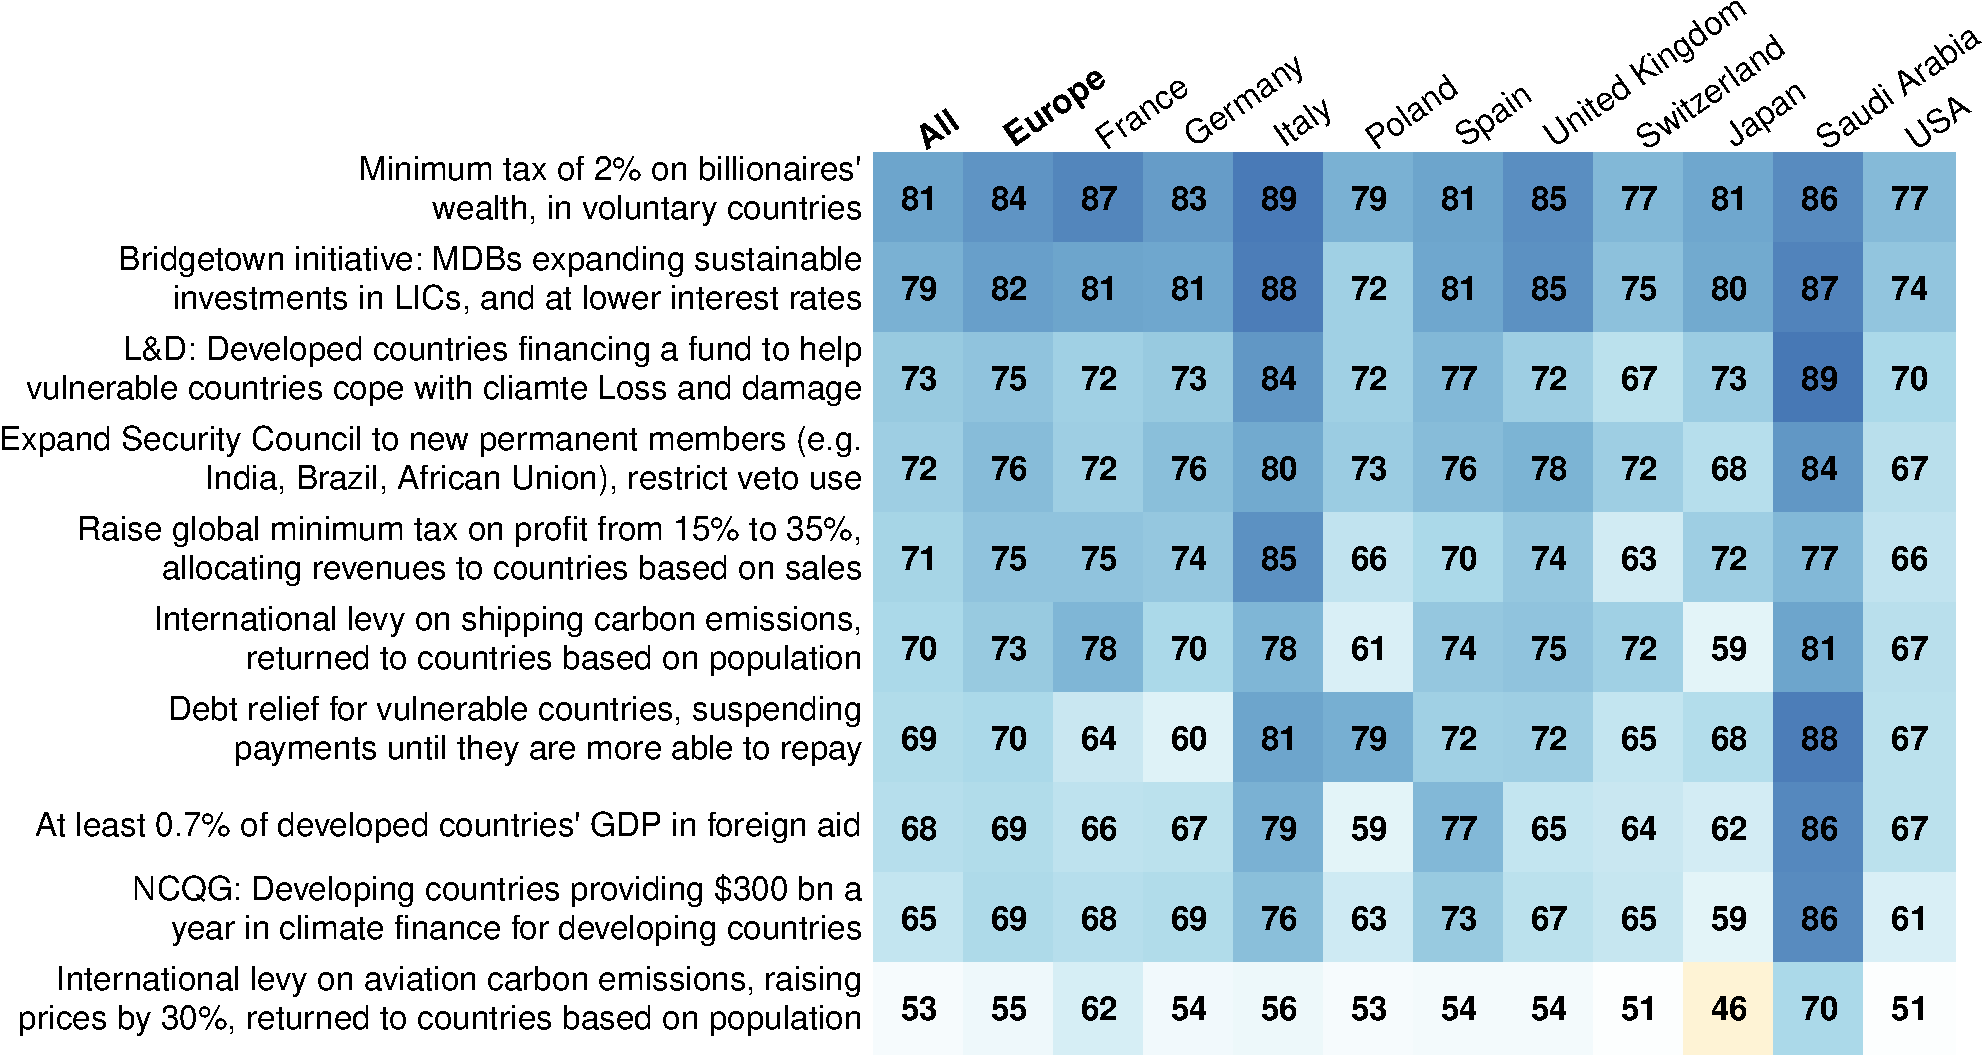
\includegraphics[width=.87\textwidth]{../figures/country_comparison/solidarity_support_share}}
% \bbvs
% \ip 
% \ee
\end{frame}

\begin{frame}{Testing warm glow} 
  \centering If \textit{warm glow}, support might dissipate when...
    \begin{figure}
% \caption{}
\begin{subfigure}{.38\textwidth}
  \caption[]{\normalsize \blue{Moral substitute}: ...the policy is replaced a less costly substitute with the same moral appeal}
  \bbvs \ip \textit{Donation lottery} treatment: Choose share of \$100 prize to donate to plant trees.
  \ip H5a: Support for GCS no lower in the treated group.
  \ee
  \vspace{3.8cm}
  % \includegraphics[width=\textwidth]{}
\end{subfigure} \quad \pause
\begin{subfigure}{.59\textwidth}
  \caption[]{\normalsize \blue{Realism}: ...the policy materializes}
  \bbvs \ip \textit{Information} treatment: ``countries have agreed to demonstrate some degree of solidarity in addressing global challenges.  Negotiations are ongoing to implement specific mechanisms for sustainable development.'' Examples:
  \bbvs \ip IMO shipping levy
  \ip 0.7\% ODA commitment
  \ip Climate finance commitment
  \ip Minimum corporate tax
  \ip Brazil proposal at G20 of taxing billionaires
  \ip UN Pact for the Future foreseeing Security Council reform
  \ip Bridgetown initiative to finance sustainable development
  \ee
  \ip H5b: Info increases belief in likelihood of global redistribution but does not reduce support for plausible global policies
  \ee
\end{subfigure}
\end{figure}
\end{frame}

\begin{frame}{No evidence of warm glow\label{warm_glow}} 
    \begin{figure}
% \caption{}
\begin{subfigure}{.47\textwidth}
  \caption[]{Effect of a \blue{\textit{Donation lottery} treatment} on support for the \rose{Global Climate Scheme}: +3p.p.*** \quad \green{\checkmark H5a}}
  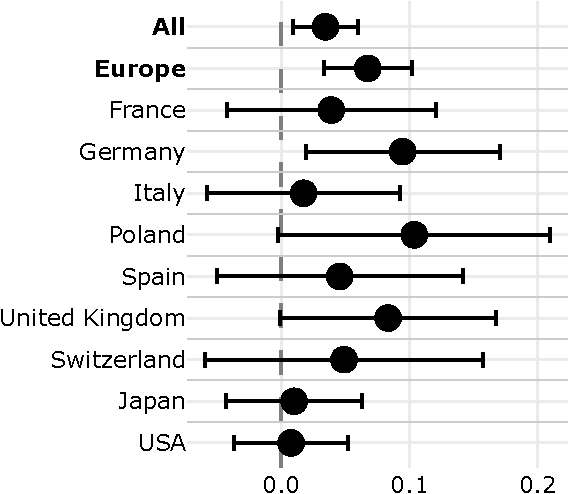
\includegraphics[width=\textwidth]{../figures/country_comparison/gcs_support_by_variant_warm_glow.pdf}
\end{subfigure} \quad \pause
\begin{subfigure}{.47\textwidth}
  \caption[]{Effect of \blue{information about ongoing global redistribution} initiatives on the share of plausible \rose{global policies} supported: +1p.p.** \quad \green{\checkmark H5b} \hyperlink{2SLS}{\beamergotobutton{2SLS}}}
  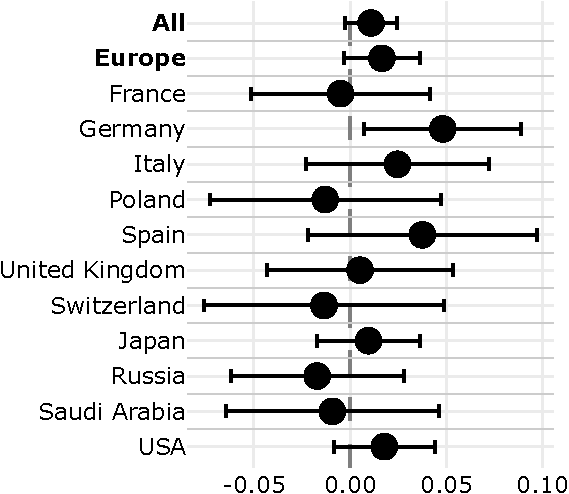
\includegraphics[width=\textwidth]{../figures/country_comparison/share_solidarity_supported_by_info_solidarity.pdf}
\end{subfigure}
\end{figure}
\end{frame}

\begin{frame}{NCQG}
\centering
\only<+>{ 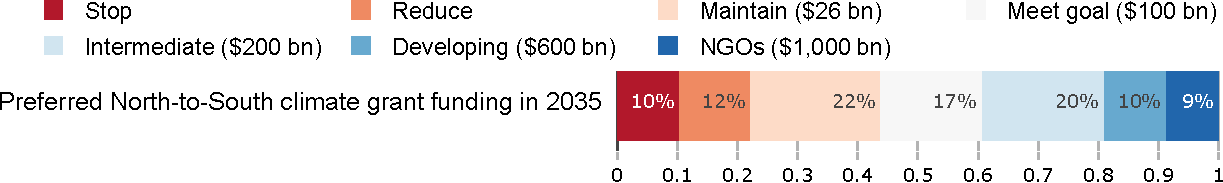
\includegraphics[height=.9\textheight]{../figures/all/ncqg}} 
\only<+>{ 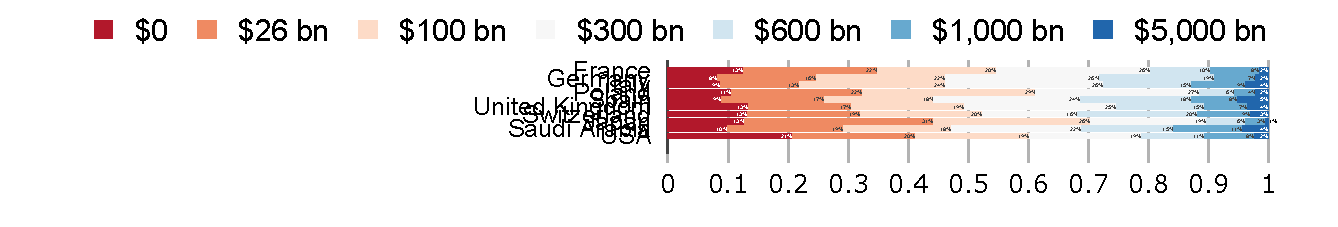
\includegraphics[height=.9\textheight]{../figures/all/ncqg_full}} 
\end{frame}

\begin{frame}{BAU vs. sustainable future}
BAU future:
\begin{itemize}
    \item No additional policies to address climate change or inequality. 
    \item Stable carbon emissions. \blue{+3\textdegree{}C} warming by 2100, causing more severe natural disasters.
    \item \blue{People maintain the same lifestyles} as in 2025, such as driving gasoline cars.
\end{itemize}
Sustainable future:
\begin{itemize}
    \item \blue{Worldwide policies} to limit global warming to +2\textdegree{}C and reduce inequality.
    \item Reduced global carbon emissions, in line with climate target.
    \item \blue{Taxes on millionaires} funding heat pumps, building insulation, and public transport.
    \item All cars electric by 2045, priced like today's gasoline cars.
    \item Heating fuel, air travel, and beef \blue{prices gradually double}. 
     %As a result, 50\% less flying and meat consumption, and more public transport use.
    \item Lower sales tax on non-polluting goods \blue{preserves overall purchasing power}.
\end{itemize}
\makebox[\textwidth][c]{
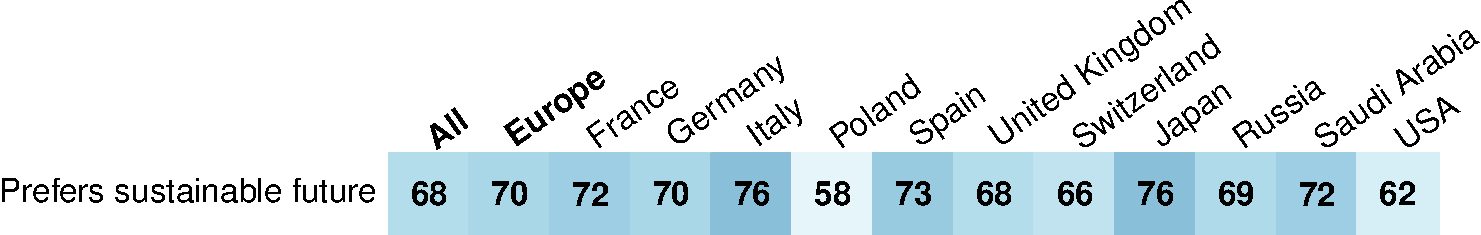
\includegraphics[width=\textwidth]{../figures/country_comparison/sustainable_future_positive.pdf}} 
% \bbvs
% \ip 
% \ee
\end{frame}

\begin{frame}{Why help LICs?}
    % Some people think that high-income countries should support low-income countries. \nAmong the different reasons given, which ones do you agree with? (Multiple answers possible)
\makebox[\textwidth][c]{ 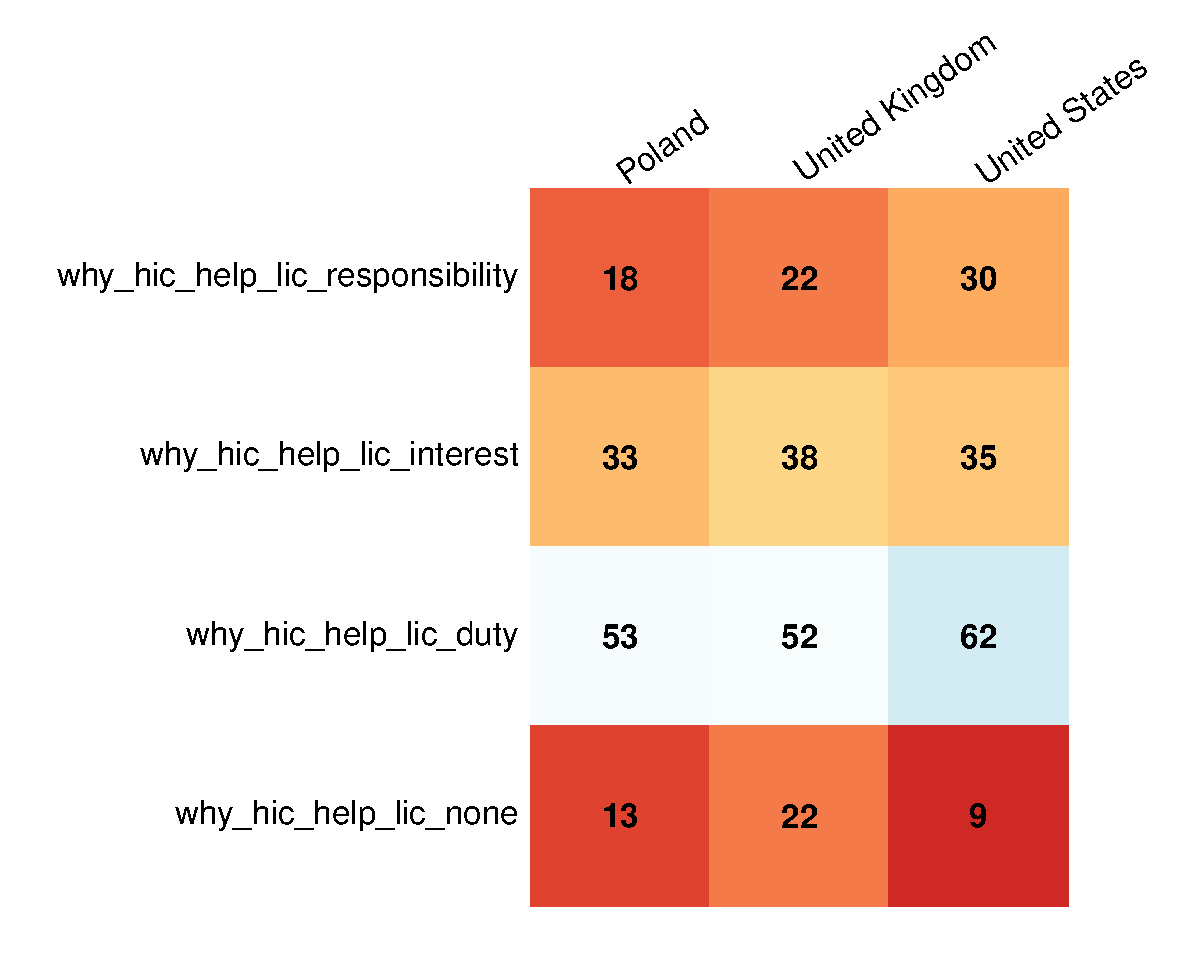
\includegraphics[width=\textwidth]{../figures/country_comparison/why_hic_help_lic_positive.pdf}}
\end{frame}

\begin{frame}{Preferred means of transfers}
    \vspace*{.5cm}
\centering How do you evaluate each of these channels to transfer resources to reduce poverty in LICs?\\ Share of \textit{Right} or \textit{Best} way (other options: \textit{Wrong} or \textit{Acceptable} way).
\makebox[\textwidth][c]{ 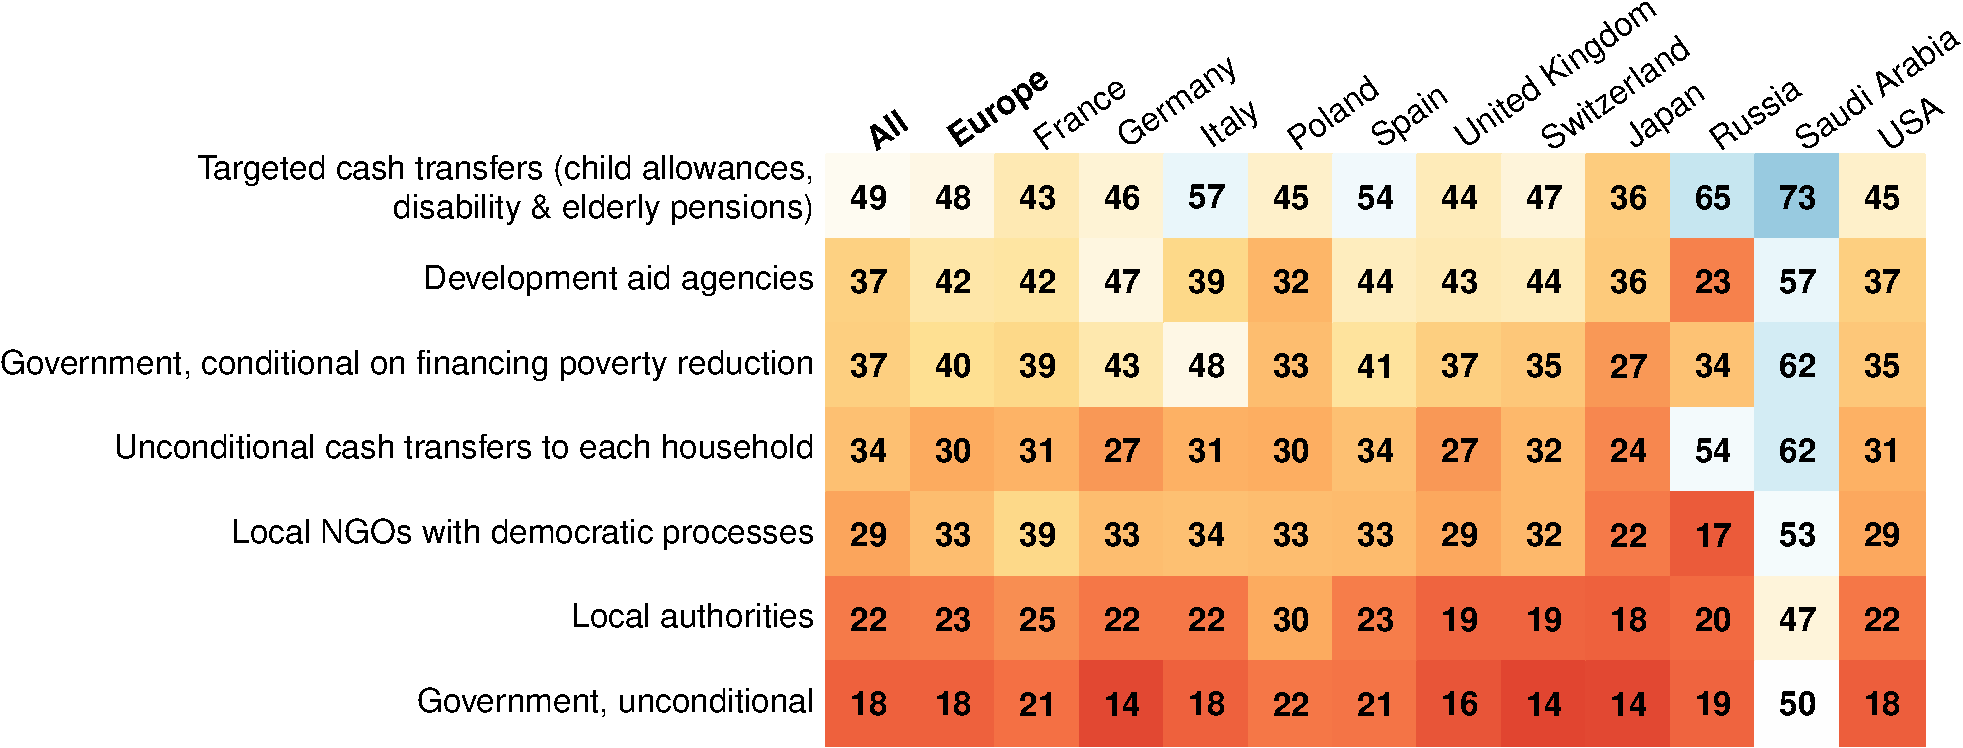
\includegraphics[width=\textwidth]{../figures/country_comparison/transfer_how_positive}}
% \bbvs
% \ip 
% \ee
\end{frame}

% Order questions in questionnaire:
% convergence
% movement
% vote_intl
% why_help
% reparations
% custom redistr
% moral circle
% my taxes

\begin{frame}{A humanist movement}
\centering If there was a worldwide movement in favor of a global program to tackle climate change, implement taxes on millionaires and fund poverty reduction in low-income countries, to what extent would you be willing to be part of that movement? (Multiple answers possible)
\makebox[\textwidth][c]{ 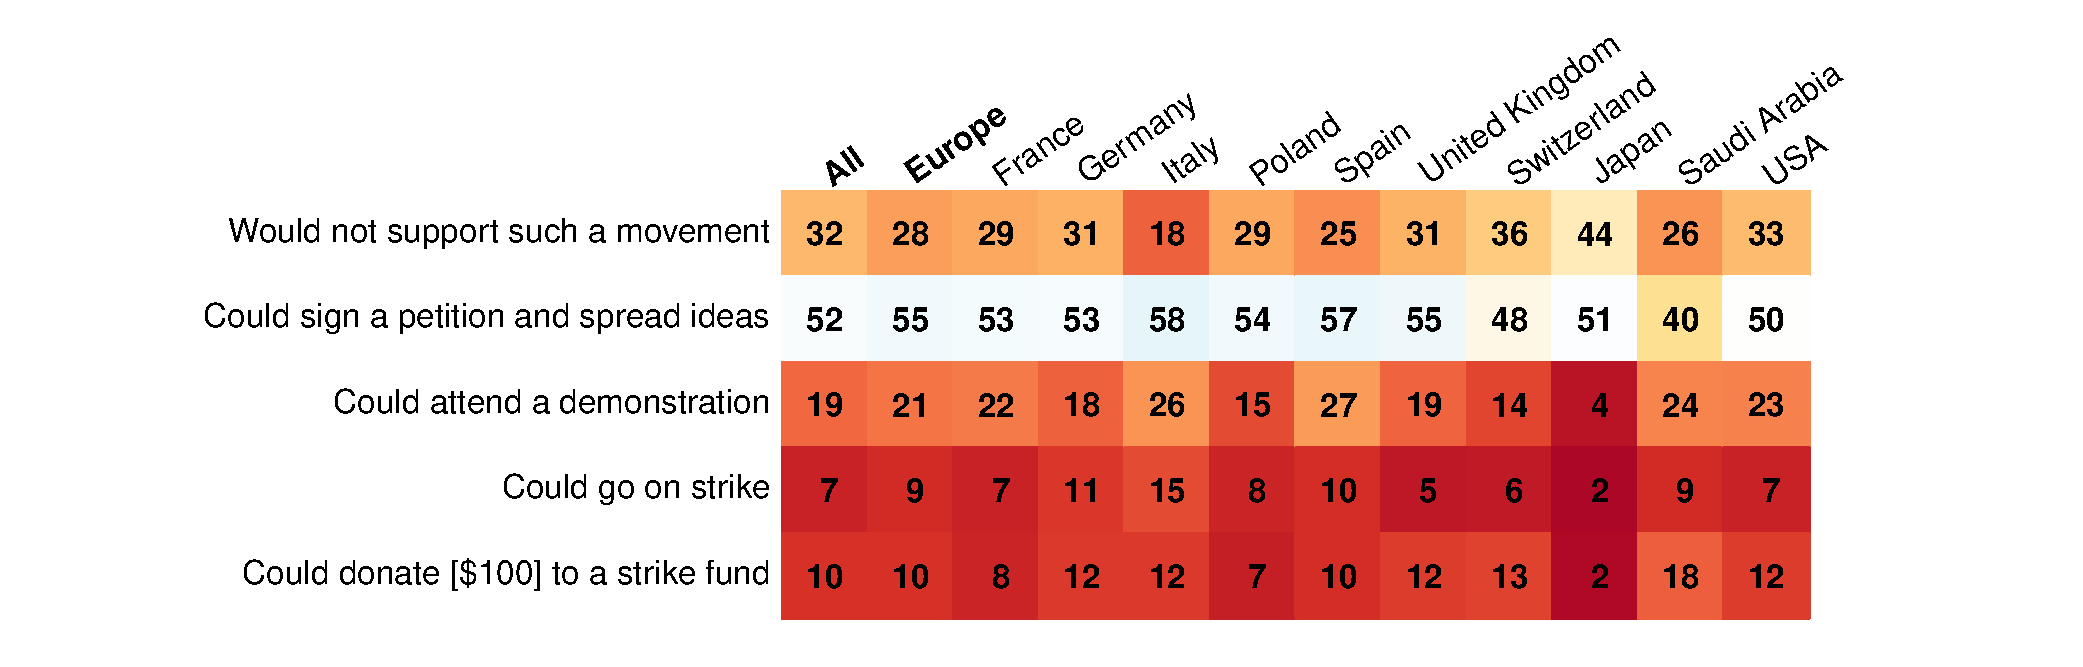
\includegraphics[width=\textwidth]{../figures/country_comparison/global_movement_positive.pdf}}
% \bbvs
% \ip 
% \ee
\end{frame}

\begin{frame}{Importance on voting}
\makebox[\textwidth][c]{ 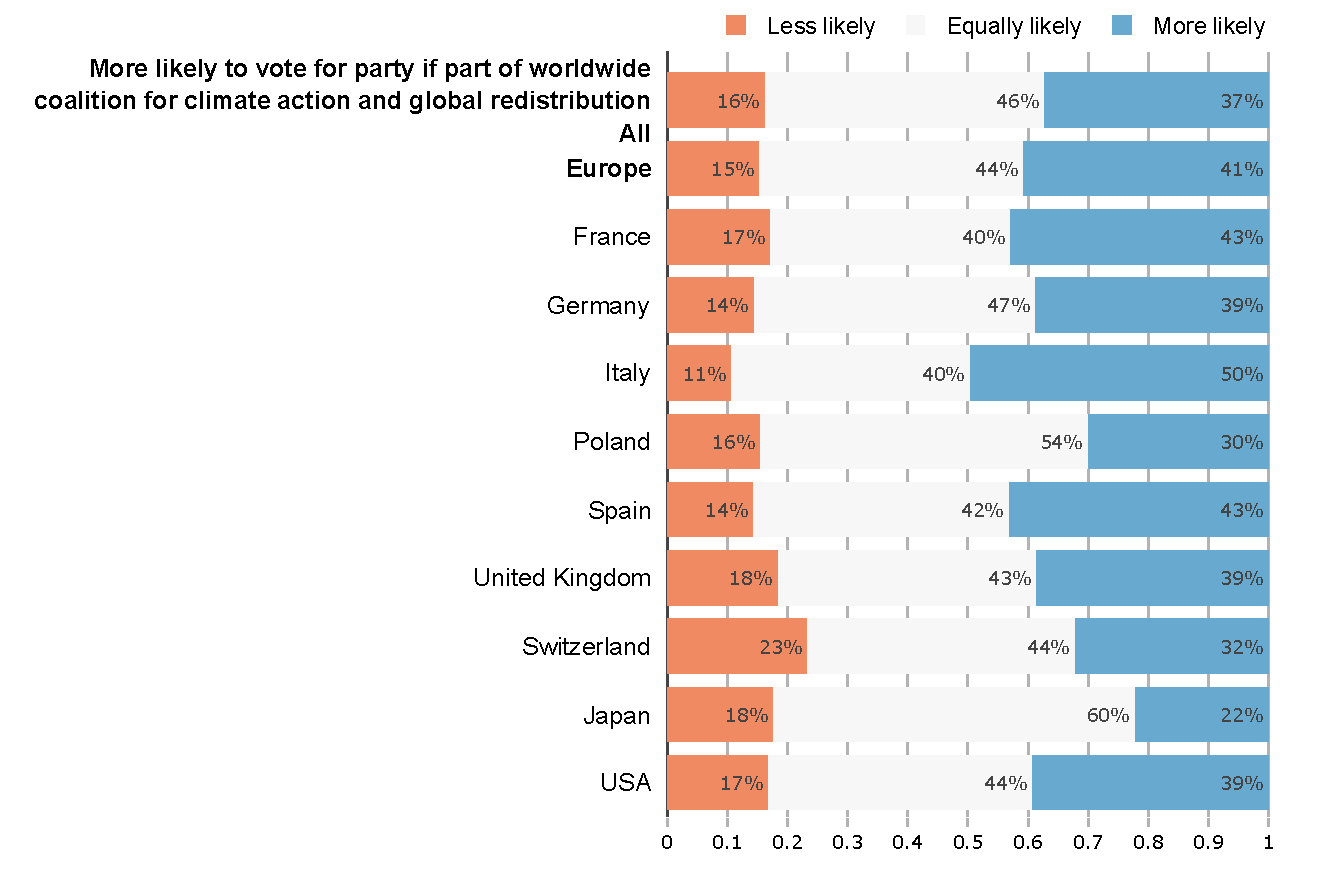
\includegraphics[height=.9\textheight]{../figures/all/vote_intl_coalition.pdf}}
% \bbvs
% \ip 
% \ee
\end{frame}

\begin{frame}{Moral circle}
\makebox[\textwidth][c]{ 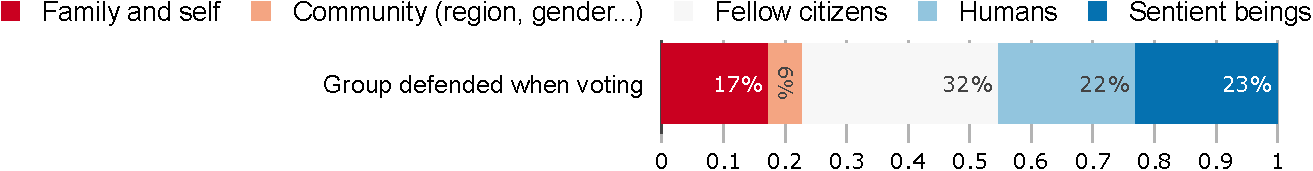
\includegraphics[height=.9\textheight]{../figures/all/group_defended}}
% \bbvs
% \ip 
% \ee
\end{frame}

\begin{frame}{Radical redistribution}
\makebox[\textwidth][c]{ 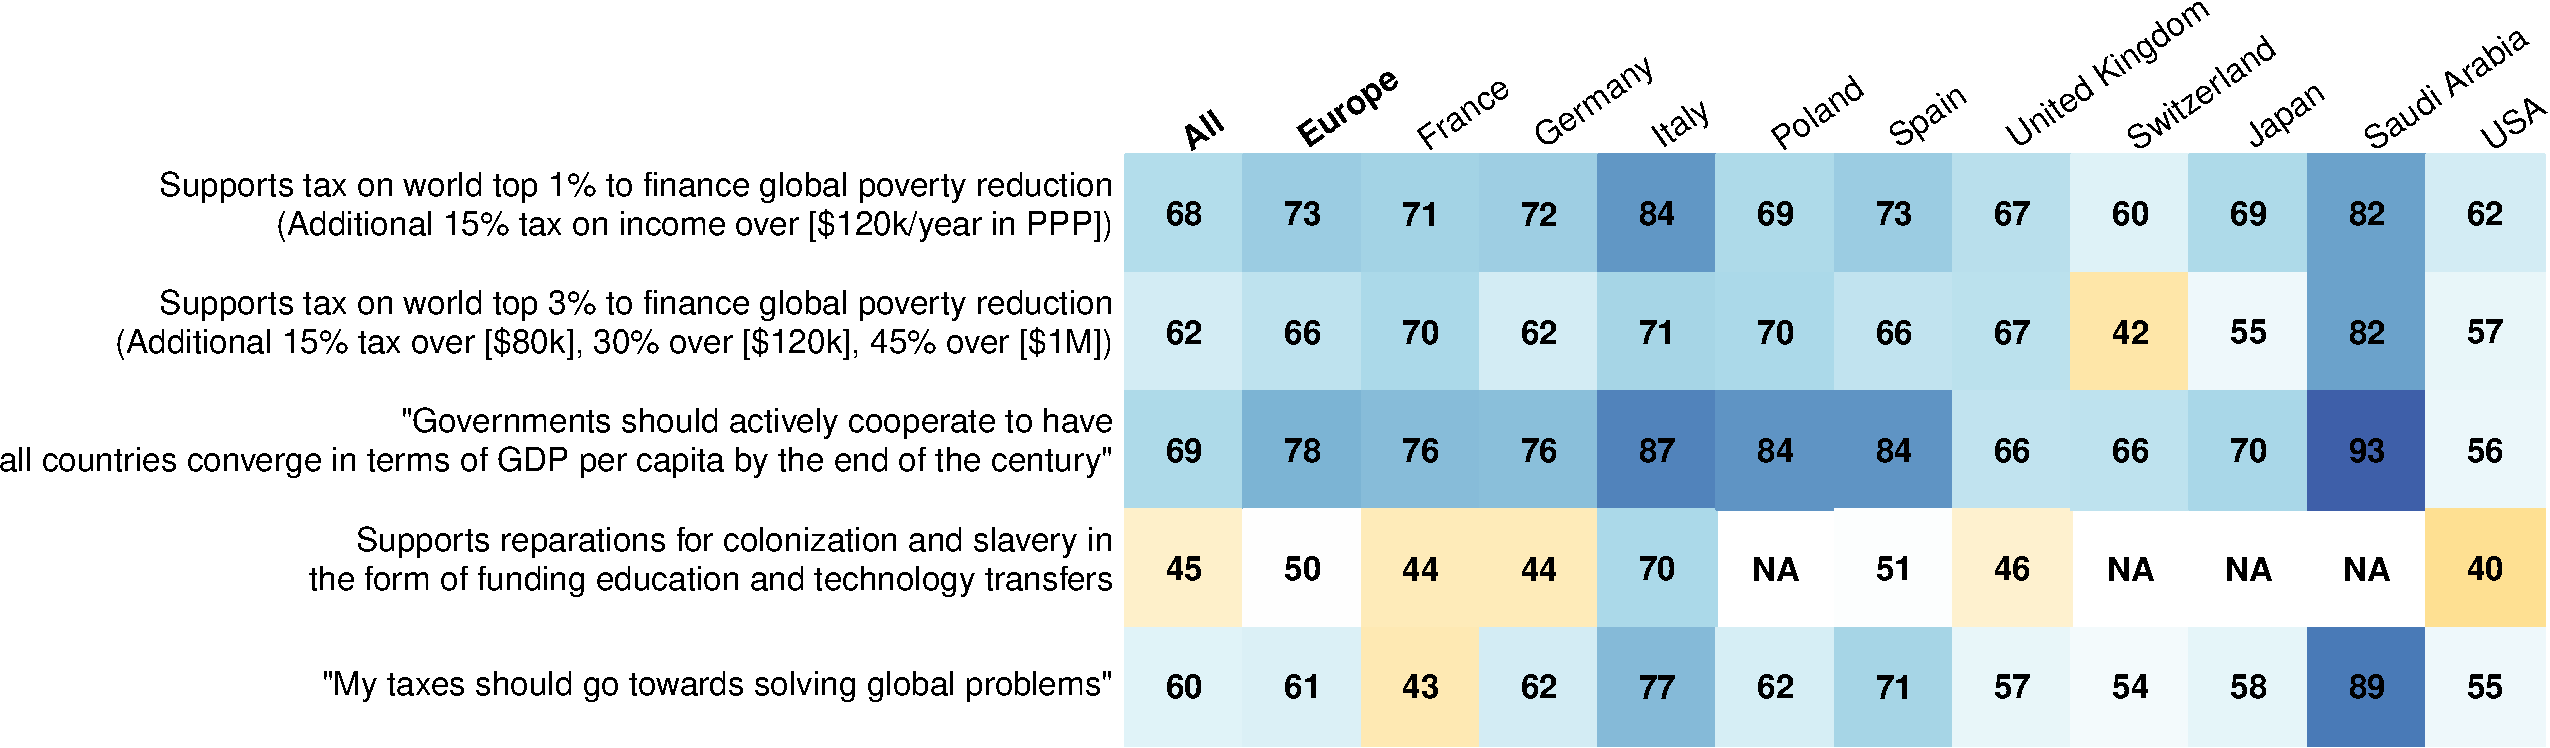
\includegraphics[width=\textwidth]{../figures/country_comparison/radical_redistr_few_share}}
% \bbvs
% \ip 
% \ee
\end{frame}

% TODO refaire vidéo en commençant par expliquer les axes
% TODO add link to interactive graph
\begin{frame}{Custom redistribution \href{run:../figures/questionnaire/survey_custom_redistr.mp4}{\beamergotobutton{Video}} \href{https://bit.ly/custom_redistr}{\beamergotobutton{bit.ly/custom\_redistr}}} 
    \centering
    \only<+>{\begin{figure}
    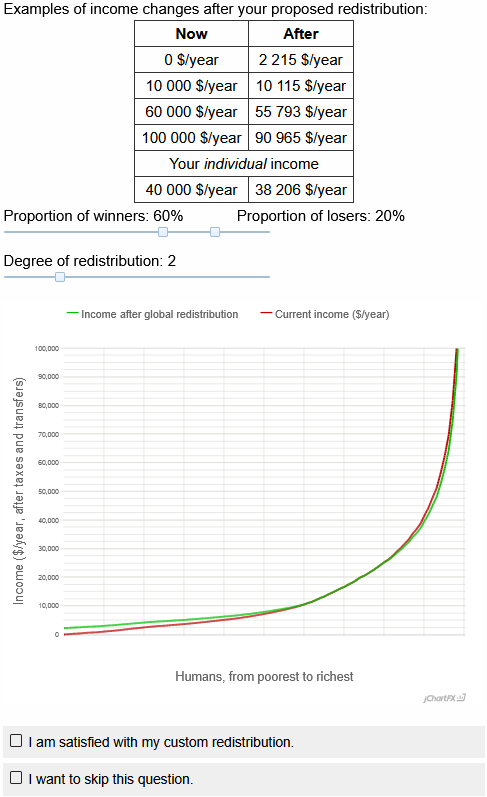
\includegraphics[height=.93\textheight]{../figures/questionnaire/survey_custom_redistr_bottom.png}\end{figure}}
    \only<+>{\begin{figure}\caption{Redistribution with median preferred parameters (among satisfied): 
    winners 49\%; losers: 18\%; degree: 5.}
    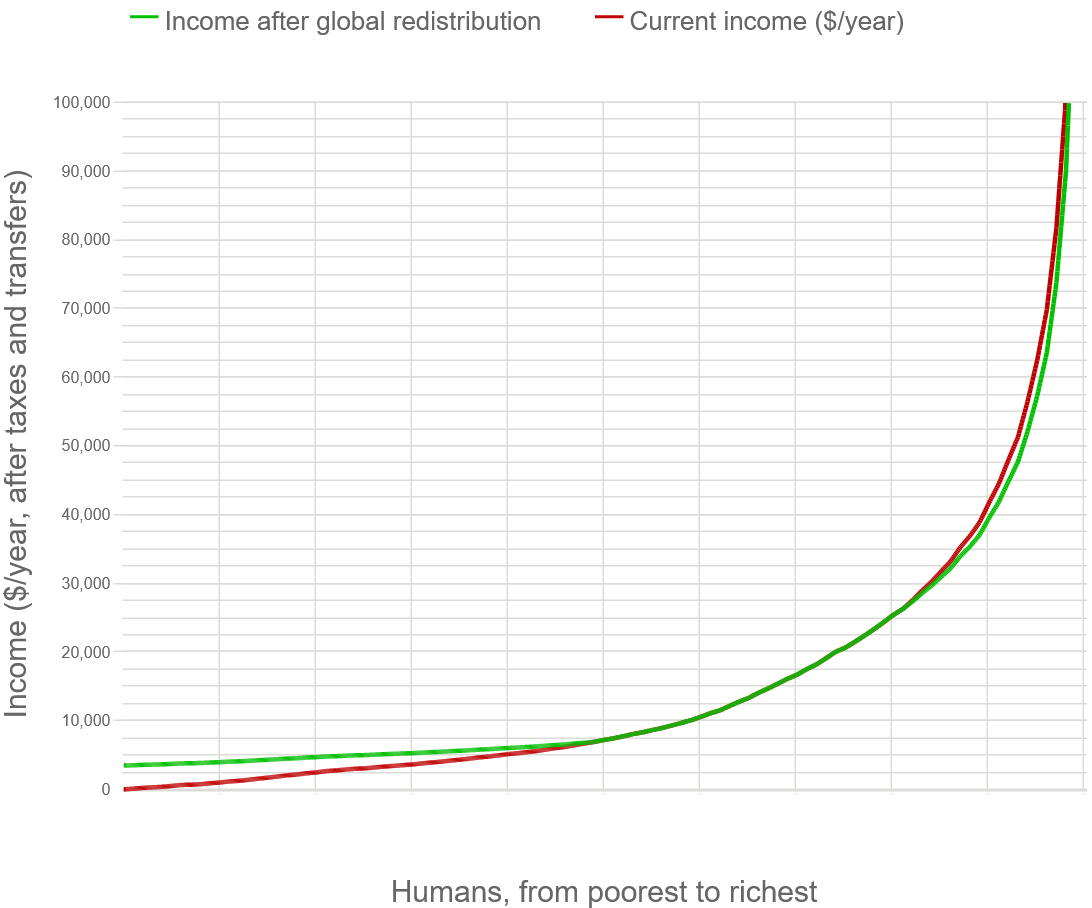
\includegraphics[height=.83\textheight]{../figures/questionnaire/survey_custom_redistr_median_zoom.png}\end{figure}}
    \only<+>{
        \bbs \ip 56\% satisfied; 43\% skipped
        \ip Share satisfied among:\\non-voters: 50\%; left: 60\%, right: 53\%, far right: 58\%.
        \ip \blue{49\% lose} from their custom redistribution while only \rose{9\% win}.
        \ip Average custom redistribution:
        \bbs \ip \blue{Minimal income: \$243/month (i.e. \$8/day)}
        \ip \blue{5\% of world income transferred} from top 28\% \rose{to bottom 72\%}
        \ee         \ee
    }
    % \only<+>{\caption{Average preferred redistribution} % TODO
    % 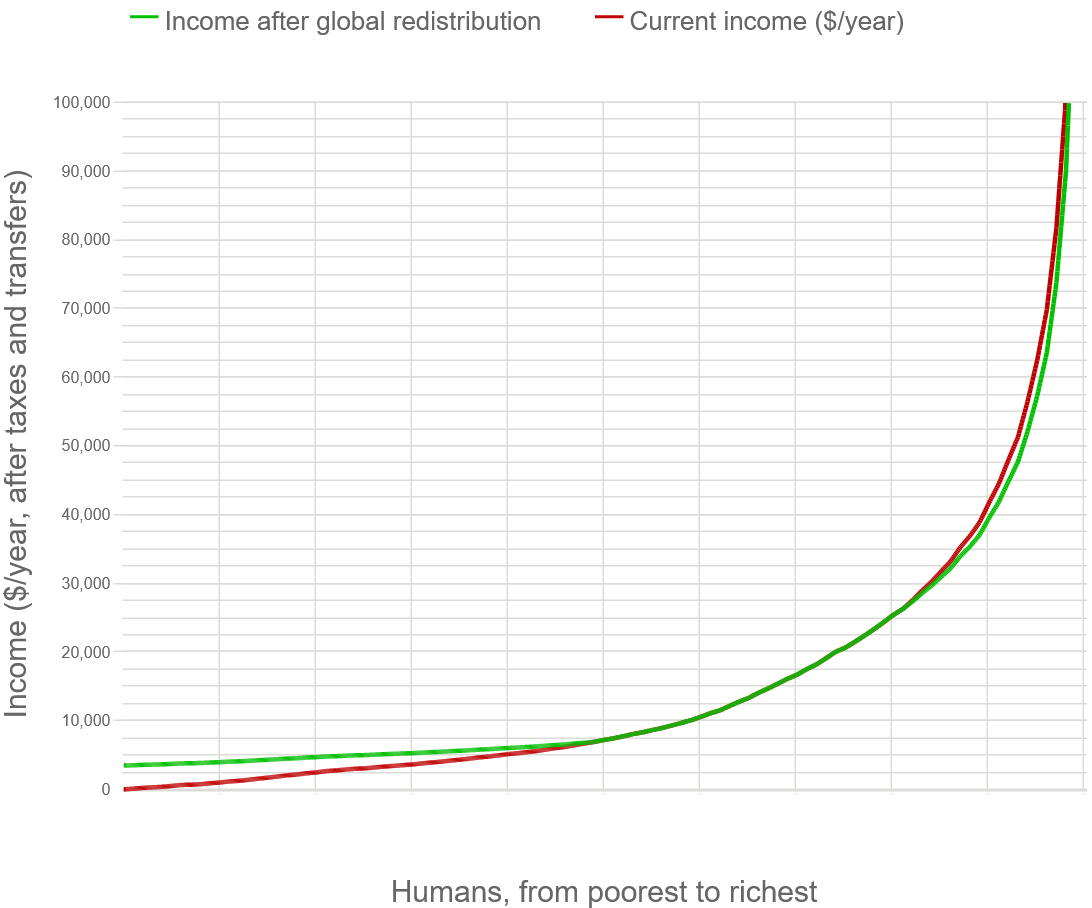
\includegraphics[width=\textwidth]{../figures/questionnaire/survey_custom_redistr_median_zoom.png}}
\end{frame}

\begin{frame}{Conclusion}
% \makebox[\textwidth][c]{ \includegraphics[width=\textwidth]{../figures/country_comparison/}}
\bbs
\ip Global poverty seen as big injustice but not a salient concern.
\ip Strong majority support for globally redistributive policies.
\ip Support reduces (only) slightly when fewer countries participate.
\ip Support is genuine. No evidence of warm glow.
\ip Global redistribution is a vote-determining issue for many people. % Majority on the left? What about abstentionnist?
\ip Most agree global sustainability is a duty.
\ip Most agree they should contribute themselves.
\ee
\end{frame}

\appendix 
\section{Appendix}

\begin{frame}{Conjoint analyses\label{conjoint_countries} \hyperlink{conjoint_country}{\beamergotobutton{Go back}}} 
    \begin{figure}
\only<+>{\caption{Conjoint analysis in France (Average Marginal Component Effect)} 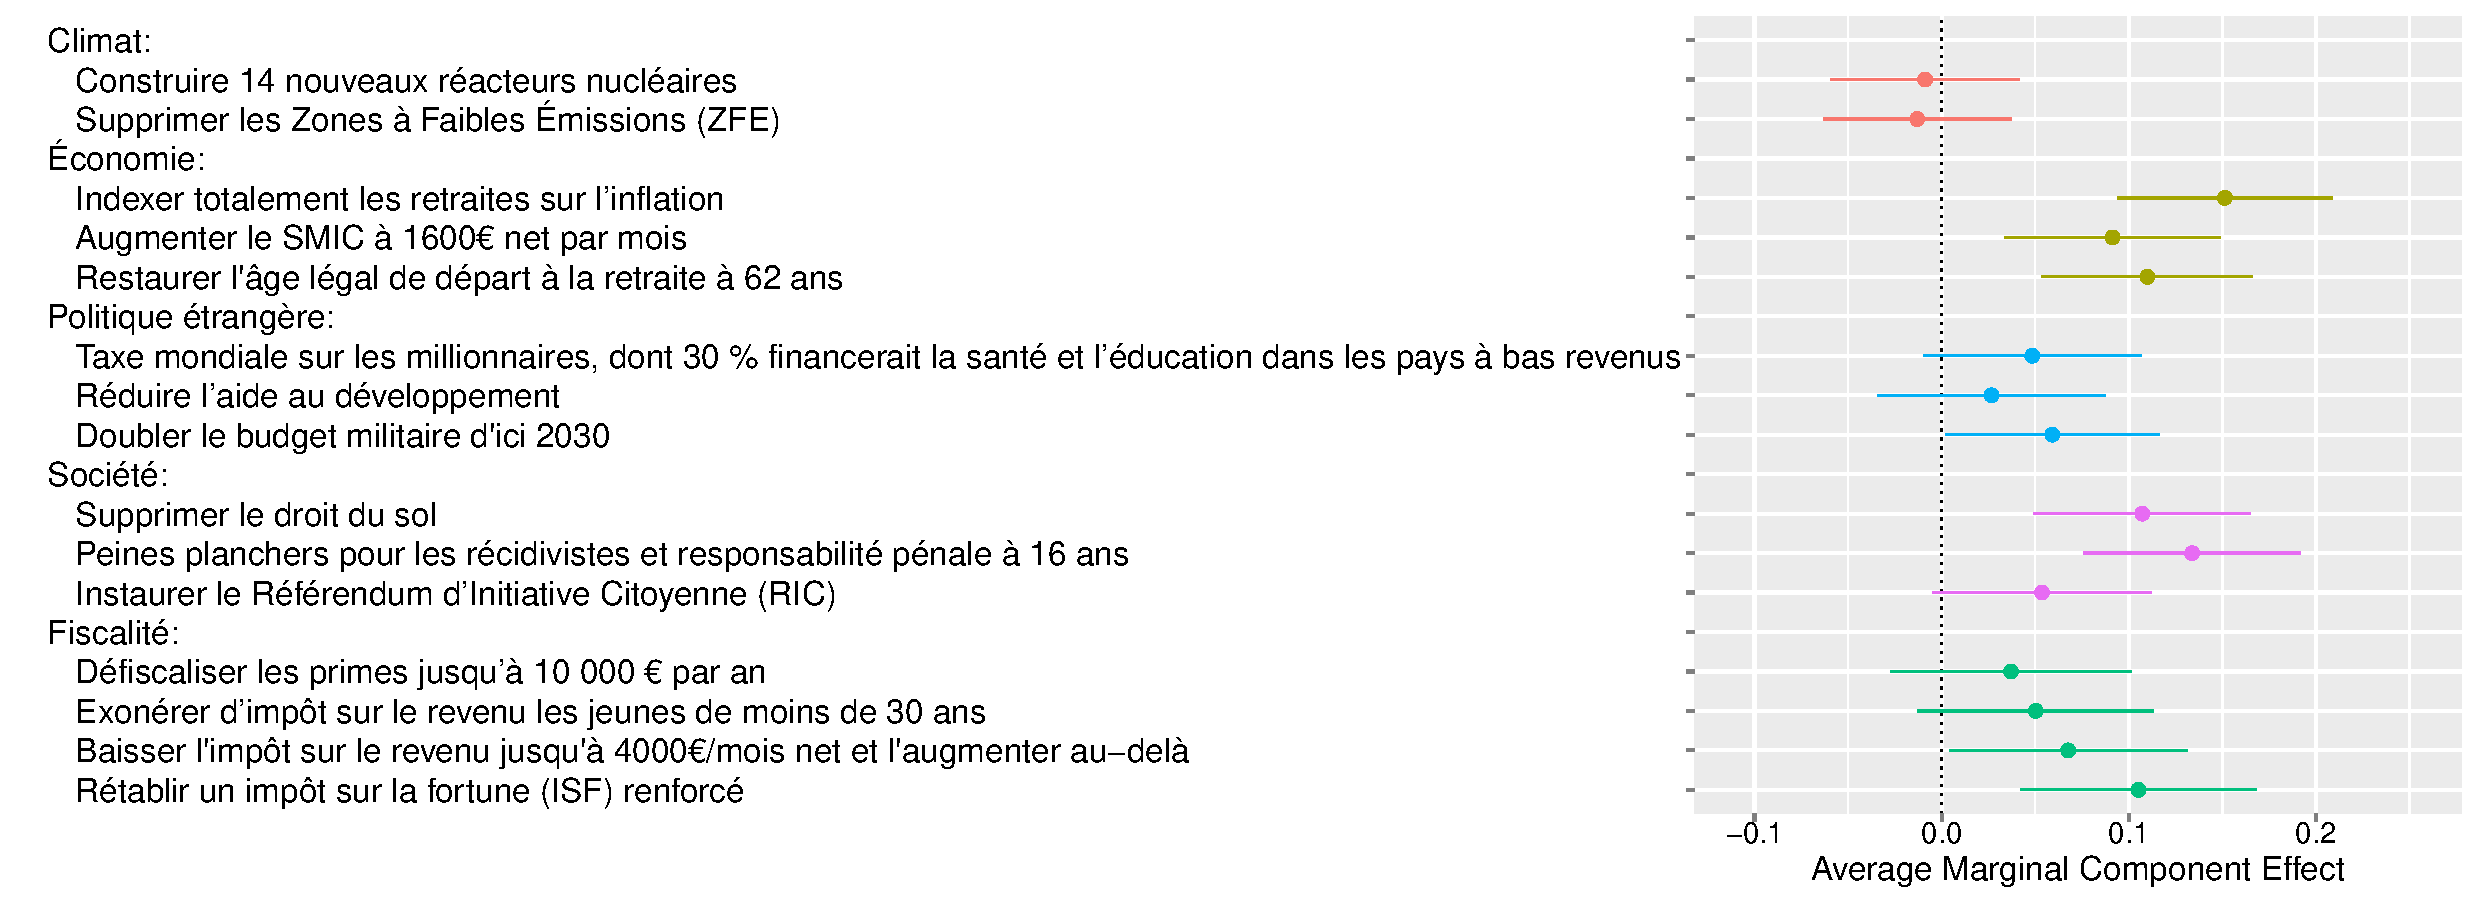
\includegraphics[width=\textwidth]{../figures/FR/conjoint_FR.pdf}}
\only<+>{\caption{Conjoint analysis in Germany (Average Marginal Component Effect)} 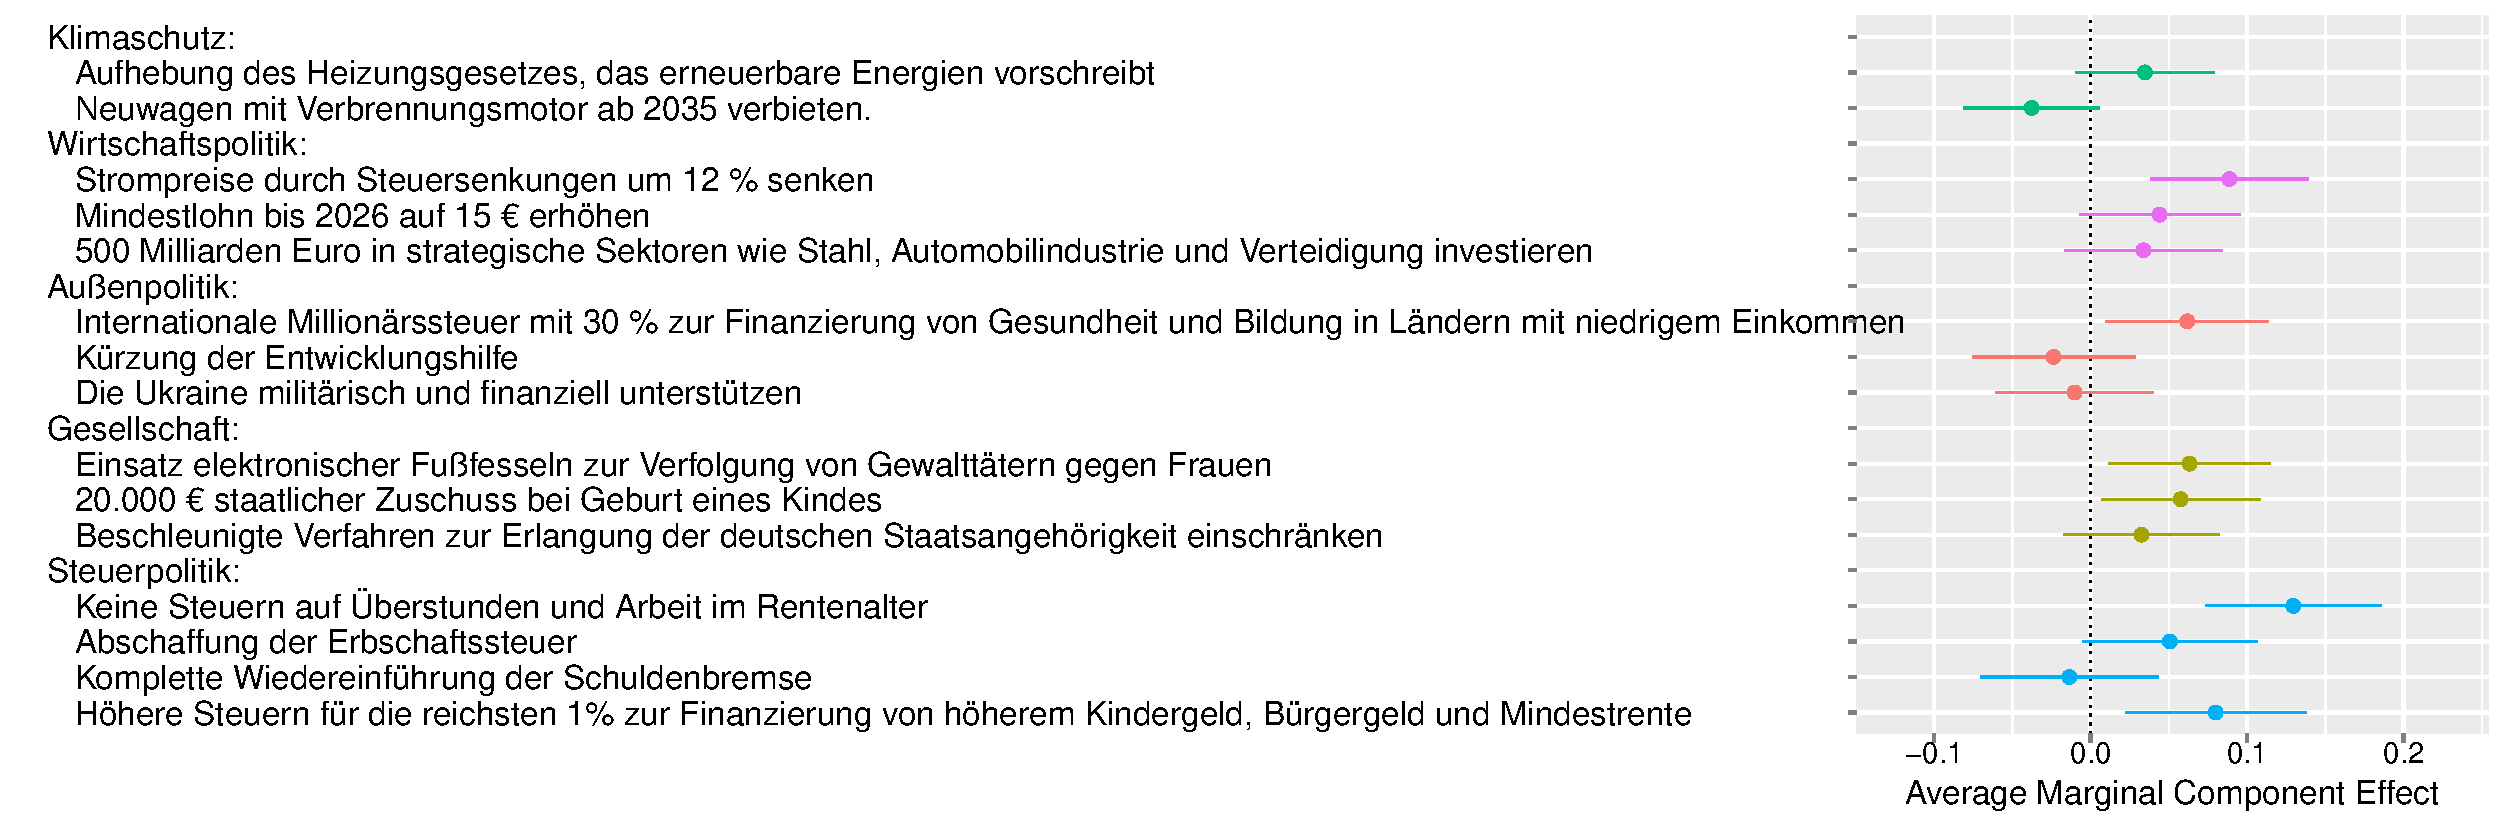
\includegraphics[width=\textwidth]{../figures/DE/conjoint_DE.pdf}}
\only<+>{\caption{Conjoint analysis in Italy (Average Marginal Component Effect)} 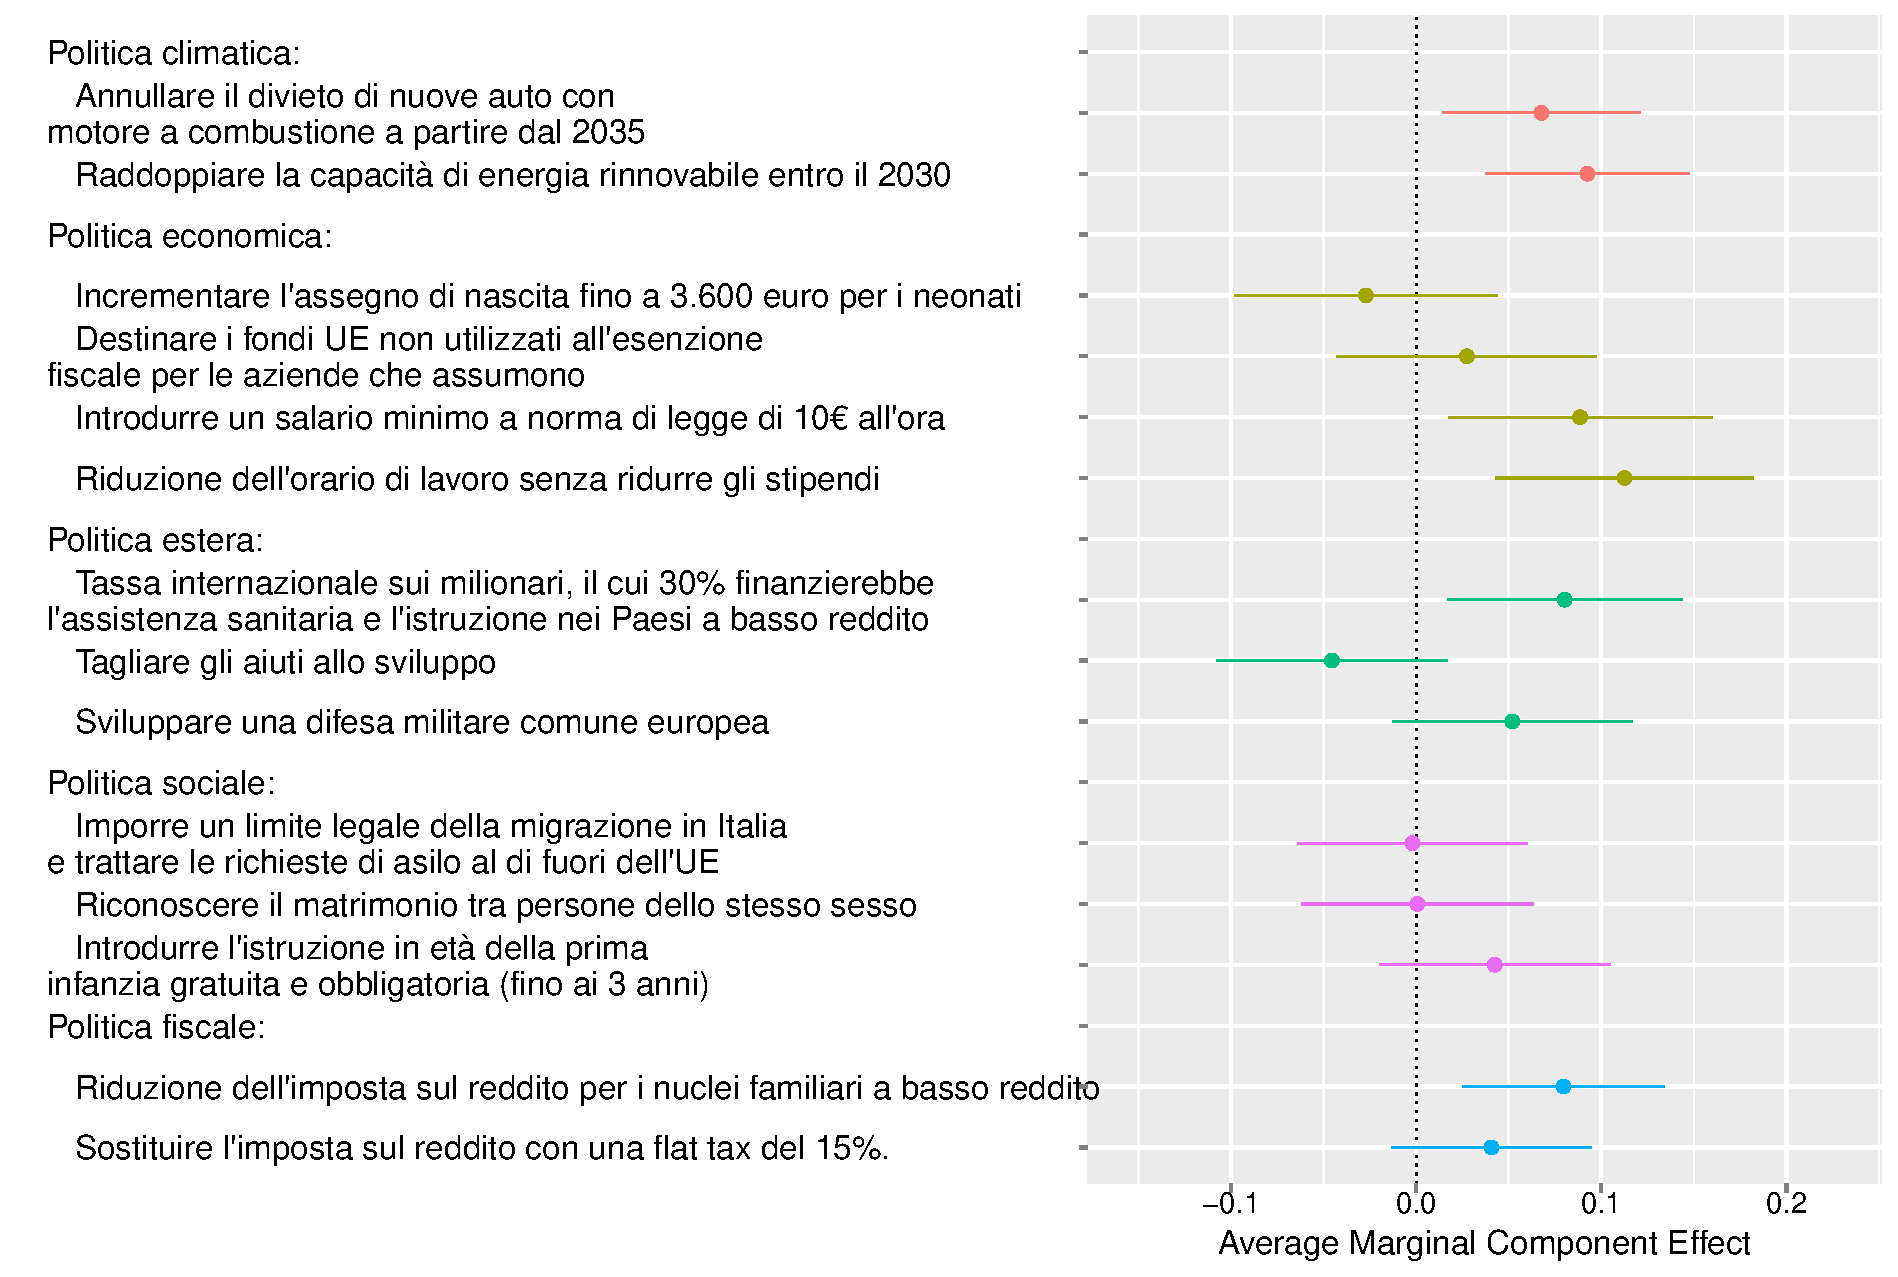
\includegraphics[width=\textwidth]{../figures/IT/conjoint_IT.pdf}}
\only<+>{\caption{Conjoint analysis in Poland (Average Marginal Component Effect)} 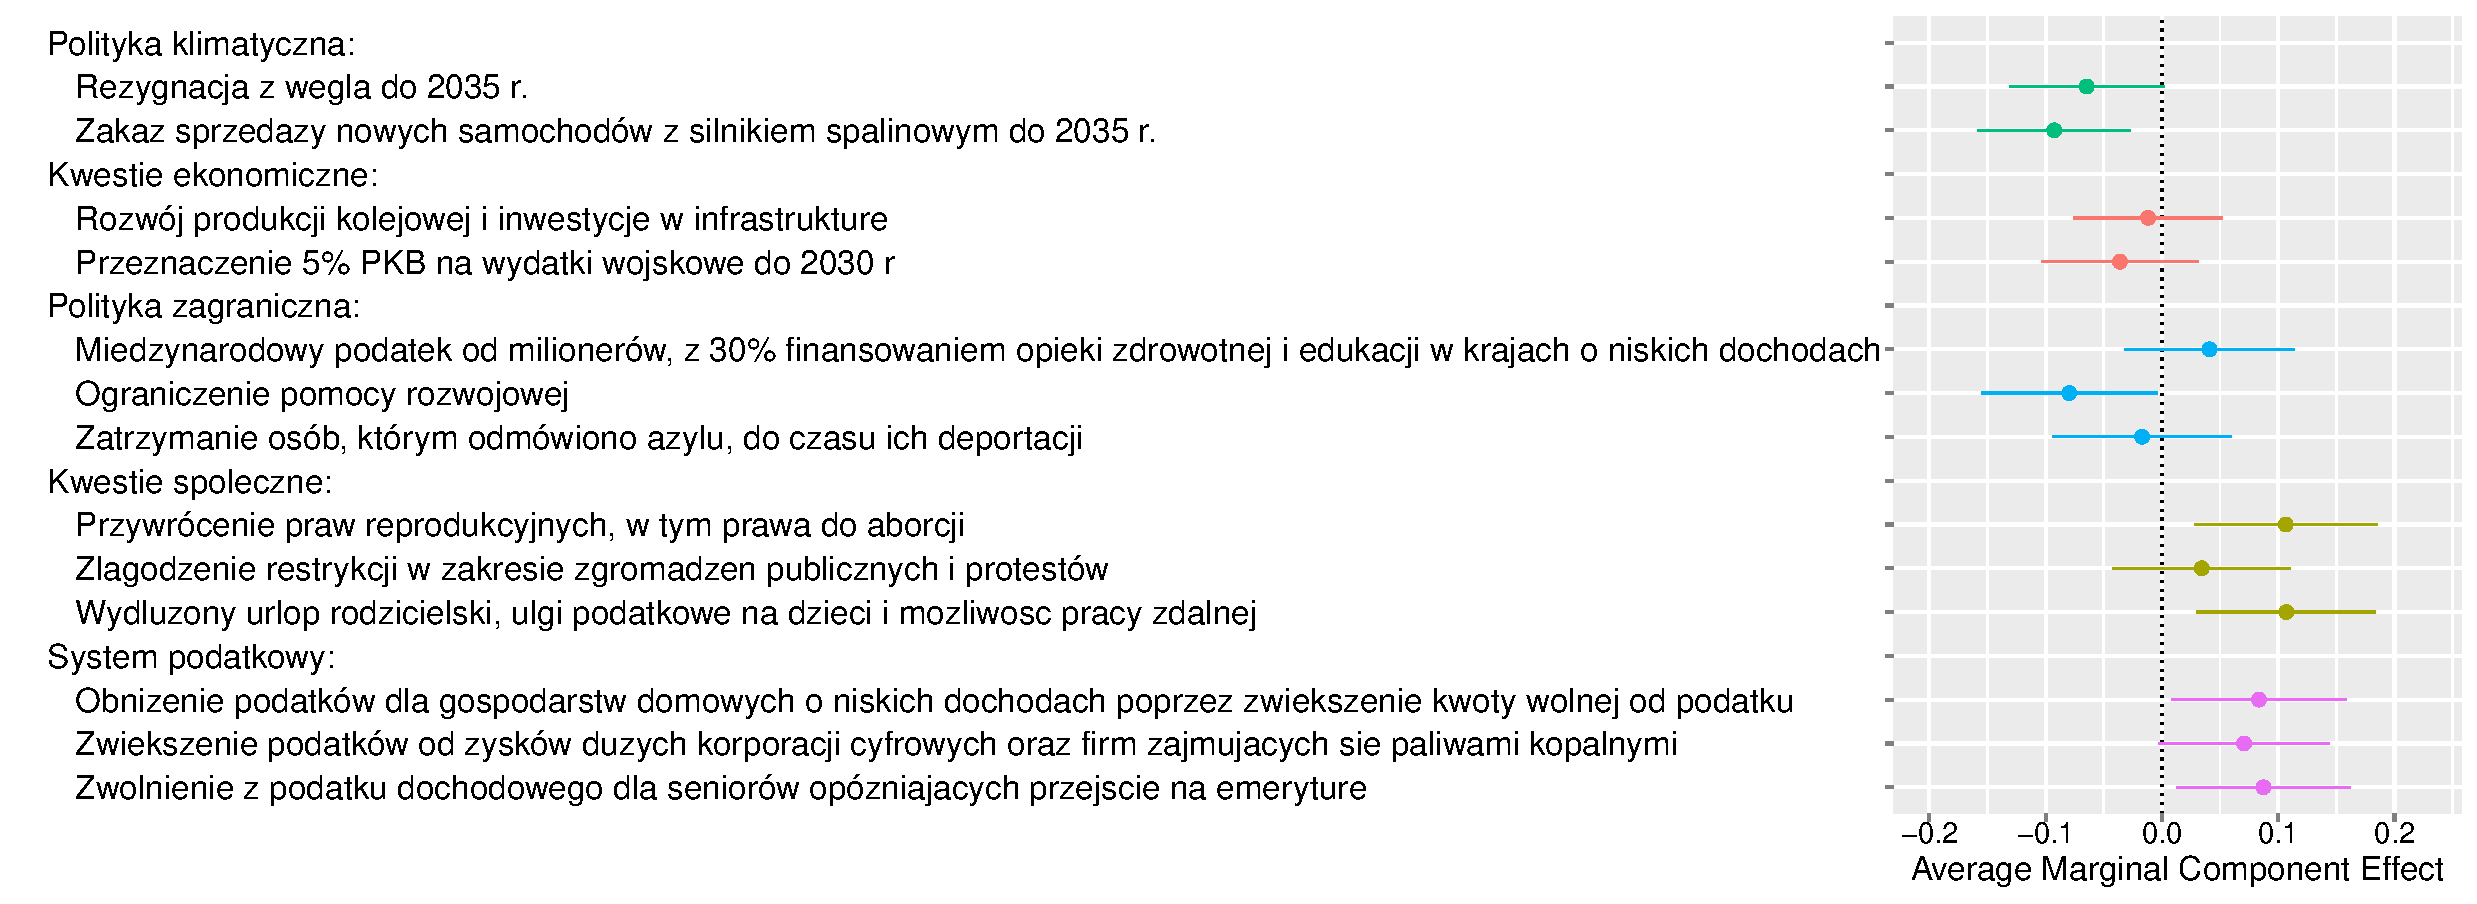
\includegraphics[width=\textwidth]{../figures/PL/conjoint_PL.pdf}}
\only<+>{\caption{Conjoint analysis in Spain (Average Marginal Component Effect)} \includegraphics[width=\textwidth]{../figures/ES/conjoint_ES.pdf}}
\only<+>{\caption{Conjoint analysis in the UK (Average Marginal Component Effect)} \includegraphics[width=\textwidth]{../figures/GB/conjoint_GB.pdf}}
\only<+>{\caption{Conjoint analysis in Switzerland (Average Marginal Component Effect)} \includegraphics[width=\textwidth]{../figures/CH/conjoint_CH.pdf}}
% \only<+>{\caption{Conjoint analysis in Japan (Average Marginal Component Effect)} \includegraphics[width=\textwidth]{../figures/JP/conjoint_JP.pdf}}
\only<+>{\caption{Conjoint analysis in the U.S. (Average Marginal Component Effect)} \includegraphics[width=\textwidth]{../figures/US/conjoint_US.pdf}}
\end{figure}
\end{frame}

\begin{frame}{Global Climate Scheme question (in the U.S.)\label{gcs_question} \hyperlink{cs}{\beamergotobutton{Go back}}}
  \footnotesize
  Do you support the following policy?\\
  
  To ensure that you have attentively read the description, \textbf{we will ask some comprehension questions later in the survey: those who get correct answers can win \$100.}\\ 
  
\vspace{.2cm}
  \textbf{Global Climate Scheme:} \\ 

\vspace{.2cm}
  In 2015, all countries agreed to contain global warming ``well below +2\textdegree{}C''. To achieve this, \textbf{there is a maximum amount of greenhouse gases we can emit globally}. \\ 

\vspace{.2cm}
  To meet the climate target, a limited number of permits to emit greenhouse gases would be issued globally. Polluting firms would be required to buy permits to cover their greenhouse gas emissions. Such a policy would \textbf{make fossil fuel companies pay} for their emissions and gradually raise the price of fossil fuels. \textbf{Higher prices would encourage people and companies to use less fossil fuels, reducing greenhouse gas emissions}. \\ 

\vspace{.2cm}
  In accordance with the principle that each human has an equal right to pollute, the revenues generated by the sale of permits could finance a global basic income. \textbf{Every adult would receive \$35 per month}, thereby lifting 600 million people who earn less than \$2 a day out of extreme poverty.\\ 

  \textbf{The typical American would lose out financially \$90  per month} (as he or she would face around 2\% in price increases, which is higher than the \$35 per month they would receive).\\ 

\vspace{.2cm}
  The policy could be implemented as soon as 100 countries agree to it. Countries that would refuse to take part in the policy could face sanctions (like tariffs) from the rest of the world and would be excluded from the basic income program.\\ 
\vspace{.2cm}

  \textbf{Do you support the Global Climate Scheme?}
\end{frame}
% Version any country:
  %   To ensure that you have attentively read the description, \textbf{we will ask some comprehension questions later in the survey: those who get correct answers can win [amount_lottery: \$100].}\\ 
  
  % \textbf{Global Climate Scheme:} \\ 

  % In 2015, all countries agreed to contain global warming ``well below +2\textdegree{}C''. To achieve this, \textbf{there is a maximum amount of greenhouse gases we can emit globally}. \\ 

  % To meet the climate target, a limited number of permits to emit greenhouse gases would be issued globally. Polluting firms would be required to buy permits to cover their greenhouse gas emissions. Such a policy would \textbf{make fossil fuel companies pay} for their emissions and gradually raise the price of fossil fuels. \textbf{Higher prices would encourage people and companies to use less fossil fuels, reducing greenhouse gas emissions}. \\ 

  % In accordance with the principle that each human has an equal right to pollute, the revenues generated by the sale of permits could finance a global basic income. \textbf{Every adult would receive [amount_bi: \$35][periodicity: per month]}, thereby lifting 600 million people who earn less than \$2 a day out of extreme poverty.\\ 

  % \textbf{The typical [national: American] would lose out financially [amount_lost: \$90][periodicity: per month]} (as he or she would face around [price_increase: 2]\% in price increases, which is higher than the [amount_bi: \$35][periodicity: per month] they would receive).\\ 
  
% - People view global poverty/ineq as big injustice though not salient concern (e.g. revenue_split)
% - Strong support for global tax / GCS even with partial participation
% - No (or little) evidence of warm glow or support due to unrealism; global redistr genuinely supported (conjoint analysis)
% - People ready to sustainability and radical global redistr (for duty, not reparations)
% - People favor social protection to unconditional transfers
% - Influenced by question on revenue splits and NCQG / more or less consistent on NCQG

\begin{frame}{Plausible gobal policies\label{solidarity_support_absolute} .\hyperlink{solidarity_support_relative}{\beamergotobutton{Go back}}}
\centering Share of (somewhat or strong) \textit{support}. \\
\makebox[\textwidth][c]{ \includegraphics[width=.87\textwidth]{../figures/country_comparison/solidarity_support_positive}}
% \bbvs
% \ip 
% \ee
\end{frame}


\begin{frame}{2SLS\label{2SLS}  \hyperlink{warm_glow}{\beamergotobutton{Go back}}}  
  \small 
% Table created by stargazer v.5.2.3 by Marek Hlavac, Social Policy Institute. E-mail: marek.hlavac at gmail.com
% Date and time: jeu., juil. 10, 2025 - 19:39:53
\begin{table}[!htbp] \centering 
  \caption{Effect on support for global redistribution of believing that it is likely.} 
  \label{tab:iv} 
\begin{tabular}{@{\extracolsep{5pt}}lcccc} 
\\[-1.8ex]\hline 
\hline \\[-1.8ex] 
\\[-1.8ex] & \makecell{Believes global\\redistr. likely} & \multicolumn{3}{c}{Share of plausible global policies supported} \\ 
 & IV 1st Stage & IV 2nd Stage & OLS & Direct Effect \\ 
\\[-1.8ex] & (1) & (2) & (3) & (4)\\ 
\hline \\[-1.8ex] 
 Information treatment & 0.080$^{***}$ &  &  & 0.016$^{**}$ \\ 
  & (0.009) &  &  & (0.007) \\ 
  Believes global redistribution likely &  & \blue{0.205$^{**}$} & 0.149$^{***}$ &  \\ 
  &  & (0.082) & (0.007) &  \\ 
  (Intercept) & 0.345$^{***}$ & 0.428$^{***}$ & 0.449$^{***}$ & 0.498$^{***}$ \\ 
  & (0.006) & (0.031) & (0.004) & (0.005) \\ 
 \hline \\[-1.8ex] 
Observations & 11,000 & 11,000 & 11,000 & 11,000 \\ 
R$^{2}$ & 0.007 & 0.037 & 0.043 & 0.001 \\ 
F Statistic (df = 1; 10998) & 74.701$^{***}$ &  & 498.125$^{***}$ & 6.099$^{**}$ \\ 
\hline 
\hline \\[-1.8ex] 
\textit{Note:}  & \multicolumn{4}{r}{$^{*}$p$<$0.1; $^{**}$p$<$0.05; $^{***}$p$<$0.01} \\ 
\end{tabular} 
\end{table} 

\end{frame}


\begin{frame}{Last slide (needed)}
  
\end{frame}


% \begin{frame}{Figure with emphasis}
% 	\vspace{-.1cm}
% 	\begin{center}
% 		\begin{tikzpicture}
% 			\node[anchor=south west,inner sep=0] (image) at (0,0) {
%         %\includegraphics[trim= 0cm 0cm 0cm .7cm,clip,width=.82\paperwidth]{example}
%          };
% 			\begin{scope}[x={($0.1*(image.south east)$)},y={($0.1*(image.north west)$)}] % This adds a grey rectangle to highlight part of the figure
			
% 			\end{scope}
% 		\end{tikzpicture}
% 	\end{center}
% \end{frame}

% \begin{frame}{Columns}
% \begin{columns}
% \begin{column}{0.5\textwidth}
% \begin{figure}
% \caption{Caption}
% %\includegraphics[width=.43\paperwidth]{../figures/.png}
% \end{figure}
% \end{column}
% \begin{column}{0.5\textwidth}
% \begin{figure}
% \caption{Captions}
% %\includegraphics[width=.43\paperwidth]{../figures/.png}
% \end{figure}
% \end{column}
% \end{columns}
% \end{frame}

% \setbeamercovered{invisible}
% \begin{frame}{Proof_only_once}
%     \begin{block}{Proposition}<+->
%     Prop
%     \end{block}
%     \only<+>{\begin{proof} 
%     Proof
%     \end{proof}}
        
%     \begin{block}{Proposition}<+->
%     Prop
%     \end{block}
%     \only<+>{\begin{proof} 
%     Proof
%     \end{proof}}
% \end{frame}

% \setbeamercovered{transparent=65}
% \begin{frame}{Transparent}
% \onslide<1->
% \centering
% Text
% \onslide<2->
% \begin{table}[ht] 
% \centering
% %\caption{}
% \begin{tabular}{lcccccc}
% \toprule
% & \phantom{a}	&\multicolumn{2}{c}{Payoffs} & \phantom{a} & \multicolumn{2}{c}{Beliefs} \\										\cmidrule{3-4} \cmidrule{6-7}
% 			&&	No_project	& Project 	&&	Expert1 	& Expert2 	\\		
% Bad		&&	$0$		& $10$	    &&	$0$	        & $5$	\\		
% Neutral 	&&	$0$		& $0$	    &&	$1$	        & $0$ \\					
% Good   	&&	$0$		& $10$	    &&	$0$	        & $5$ \\				 
%  \bottomrule
% \end{tabular} 
% \label{TableExample}
% \end{table}
% \end{frame}

% \begin{frame}{Uncertainty aversion}
% \begin{itemize}[<+>]
% \item 1
% \item 2
% \end{itemize}    
% \end{frame}

% \begin{frame}{Custom_items}\label{properties}
% Link \hyperlink{proof}{\beamergotobutton{See_proof}}
% \begin{itemize}
% \item<-2> First_item_until_2 
%   \begin{itemize}[<2>]
%     \item all
%     \item at
%     \item 2
%   \end{itemize}
% \item<3> Shown_at_3
% \end{itemize}
% \visible<4>{Visible_at_4.}
% \end{frame}

% \begin{frame}{Proof \hyperlink{properties}{\beamergotobutton{Back_to_properties}}\label{proof}}
%     \begin{enumerate}[<+->]
%         \item From_1
%         \item From_2
%     \end{enumerate}
% \end{frame}

% \begin{frame}{Custom_items}
% \begin{itemize}
% \item<1-> From_1
% \item<1-> From_2
%   \begin{itemize}
%   \item<2-> From_2
%   \item<2-> From_2
%   \end{itemize}
% \vspace{0.2cm}
% \item<3-> From_3
% \vspace{0.2cm}
% \item<4-> \textbf{From_4}
% \end{itemize}
% \end{frame}


% \begin{frame}{Custom_overlays}
% \bbvs
% \ip Items_very_small_linespread \ee 
% \begin{columns}
% \begin{column}{0.5\textwidth}
% \only<1>{
% \begin{itemize}
% \ip 
% \end{itemize}
% }
% \only<2,3>{
% \begin{figure}
% %\includegraphics[width=.35\paperwidth]{../figures/.png}
% \caption{Caption}
% \end{figure}
% }
% \end{column}

% \begin{column}{0.5\textwidth}
% \only<1,3>{
% \begin{figure}
% %\includegraphics[width=.35\paperwidth]{../figures/1_IS_LM.png}
% \caption{Equillibrium in IS-LM}
% \end{figure}
% }
% \only<2>{
% \begin{itemize}
% \ip 
% \end{itemize}
% }
% \end{column}
% \end{columns}

% \end{frame}


\end{document}